%%%%%%%%%%%%%%%%%%%%%%%%%%%
%%%  Doctor of Philosophy Template
%%%  Approved for Michigan State University
%%%
%%%  Author: Alexander Lalejini
%%%  Email:  amlalejini@gmail.com
%%%
%%%  Advisor: Charles Ofria
%%%  Committee:
%%%     - Wolfgang Banzhaf
%%%     - Christoph Adami
%%%     - Richard Lenski
%%%
%%%  Last Edit:  <Keep track of your last edit date.>
%%%
%%%  Resume With: <Give yourself a pointer where to pick up.>
%%%%%%%%%%%%%%%%%%%%%%%%%%%

%%% Define the actual document parameters:
\documentclass[12pt,letterpaper,twoside]{report}


%%%  Include packages used throughout the dissertation:
\usepackage{adjustbox}
\usepackage{afterpage}
% \usepackage{algpseudocode}
\usepackage{amssymb}
\usepackage{amsmath}
\usepackage{array}
\usepackage{booktabs}
\usepackage{calc}
\usepackage[usenames,dvipsnames]{color}
\usepackage{comment}
\usepackage{csquotes}
\usepackage{epsfig}
\usepackage{fancyhdr}
\usepackage{graphicx}
\usepackage{graphics}
\usepackage[hmarginratio=1:1,margin=1in]{geometry}
\usepackage{indentfirst}
\usepackage{layout}
\usepackage{listings}
\usepackage{multirow}
\usepackage{moreverb}
\usepackage{natbib}
\usepackage{pdflscape}
\usepackage{rotating}
\usepackage{setspace}
\usepackage{subcaption}
\usepackage{tabulary}
\usepackage{tabularx}
\usepackage{tabu}
% \usepackage[euler]{textgreek}
\usepackage[flushleft]{threeparttable}
\usepackage{tocloft}
\usepackage{url}
\usepackage{hyperref}
\usepackage[table]{xcolor}
% \usepackage [latin1]{inputenc}

%%% Colors for tracking changes. %%%
%%% Use: \cut{<Text you want to cut.>} -> Makes the text red.
%%% Great for tracking changes that you send to advisor/committee.
\newcommand*\cut{\textcolor{red}}
\newcommand*\add{\textcolor{ForestGreen}}
\newcommand*\alter{\textcolor{blue}}

%%%%%%%%%%%%%%%%%%%%%%%%%%%%%%%%%%%%%%%%%%%%%%%%%%%%%%%%%%%%%%%%%%%%%%%%%%%%%%%%%%%%%

%%% Use the following to format your titles for the Table of Contents, List of Figures, List of Tables. 
%\renewcommand{\cfttoctitlefont}{\normalfont\Large\bfseries\MakeUppercase}
\setlength{\cftbeforetoctitleskip}{-0.2in}
\setlength{\cftaftertoctitleskip}{0.1875in}
\renewcommand{\cfttoctitlefont}{\hfill\Large\bfseries}
\renewcommand{\cftaftertoctitle}{\hfill}
\renewcommand{\contentsname}{\large\begin{center}{TABLE OF CONTENTS}\end{center}}

% Add dot leaders to the chapter entries in the TOC
\renewcommand{\cftchapleader}{\cftdotfill{\cftdotsep}}

\setlength{\cftbeforeloftitleskip}{-0.17in}
\setlength{\cftafterloftitleskip}{0.1875in}
\renewcommand{\cftloftitlefont}{\hfill\Large\bfseries}
\renewcommand{\cftafterloftitle}{\hfill}
\renewcommand{\listfigurename}{\large\centering{LIST OF FIGURES}}

\setlength{\cftbeforelottitleskip}{-0.33in}
\setlength{\cftafterlottitleskip}{0.3875in}
\renewcommand{\cftlottitlefont}{\hfill\Large\bfseries}
\renewcommand{\cftafterlottitle}{\hfill}
\renewcommand{\listtablename}{\large\centering{LIST OF TABLES}}

%%% Bibliography setup for TOC and The Final Page %%%%
\renewcommand{\bibname}{\vspace*{-0.95in} \large\centering{BIBLIOGRAPHY}}

%%% Put colon after figure number in the list of figures %%%
\renewcommand{\cftfigpresnum}{Figure\ }
\renewcommand{\cftfigaftersnum}{:\ }

%%% Put Table before and colon after table number in the list of tables %%%
\renewcommand{\cfttabpresnum}{Table\ }
\renewcommand{\cfttabaftersnum}{:\ }

% Put spacing after the Table #: and Figure #: in the LOF and LOT
\newlength{\mylenf}
\settowidth{\mylenf}{\cftfigpresnum}
\setlength{\cftfignumwidth}{\dimexpr\mylenf+0.35in}
\setlength{\cfttabnumwidth}{\dimexpr\mylenf+0.35in}

% Use this in conjunction with making the LOT singlespace so that long table entries are 
% single space within entries and double space between entries
\renewcommand\cfttabafterpnum{\vskip\baselineskip}

%%% Put Chapter before number in the TOC %%%
\renewcommand\chaptername{Chapter}
\renewcommand\cftchappresnum{\chaptername\space}
\setlength{\cftchapnumwidth}{\widthof{\textbf{Chapter~999~}}}

%%%%%%%%%%%%%%%%%%%%%%%%%%%%%%%%%%%%%%%%%%%%%%%%%%%%%%%%%%%%%%%%%%%%%%%%%%%%%%%%%%%%%

\fancypagestyle{mylandscape}{%
  \fancyhf{}% Clear header/footer
  \fancyfoot{% Footer
    \makebox[\textwidth][r]{% Right
      \rlap{\hspace{-.13in}%\footskip}% Push out of margin by \footskip
        \smash{% Remove vertical height
          \raisebox{\dimexpr.5\baselineskip+\footskip+.66\textheight}{% Raise vertically
            \rotatebox{90}{\thepage}}}}}}% Rotate counter-clockwise
  \renewcommand{\headrulewidth}{0pt}% No header rule
  \renewcommand{\footrulewidth}{0pt}% No footer rule
}

%%% Renew command for full page figures:
\renewcommand{\topfraction}{1.0}

% Blank page (if needed)
\newcommand\blankpage{%
    \null
    \thispagestyle{empty}%
    \addtocounter{page}{-1}%
    \newpage}

%%%%%%%%%%%%%%%%%%%%%%%%%%%%%%%%%%%%%%%%%%%%%%%%%%%%%%%%%%%%%%%%%%%%%%%%%%%%%%%%%%%%%

%%% Links to supplemental materials.
%%% (Replaceable here so you can switch to Youtube videos for your committee. 
%%% Saves you from having to go back through your individual chapters.
%%% Define a new command: \def \your command name here> {<Your text to place here.>}
% \def \cthreevideos {Videos of selected behaviors are available in the supplementary materials.  }

% \def \cfivevideos {Videos of selected behaviors are available in the supplementary materials. }

% \def \csixvideos {Videos of selected behaviors are available in the supplementary materials. }

% \def \ceightvideos {Videos of selected behaviors are available in the supplementary materials.  }

%%%%%%%%%%%%%%%%%%%%%%%%%%%%%%%%%%%%%%%%%%%%%%%%%%%%%%%%%%%%%%%%%%%%%%%%%%%%%%%%%%%%%

%%%  Set the margins as required by the MSU graduate school. 
%%%  Specifically, set the margins 1 inch top bottom and right, 
%%%  1.5 inch on left.  Now, Latex has margin origins at 1 in on the top 
%%%  and left so for 1.5 in the margin is set at 1.5 - 1 = .5 inch
%\setlength{\oddsidemargin}{.5in}   % This is the left margin for both
%\setlength{\evensidemargin}{1.5in} % even and odd pages (in case you use the book format)
\setlength{\topmargin}{0in} % Top margin (remember latex starts from 1 in)

% Pagewidth(8.5in) - textwidth(6in) - leftmargins(1.5in) = 1 inch for right margin
\setlength{\textwidth}{6.5in}

% Page height (11in) - Topmargin (1in) - Textheight (1in) = 1 in for
%                                                      bottom margin
\setlength{\textheight}{9in} %
\setlength{\footskip}{.5in}
%%% Headings are not required, thus suppress:
\setlength{\headheight}{0in} 
\setlength{\headsep}{0in}

\newsavebox{\savefig}

%%%%%%%%%%%%%%%%%%%%%%%%%%%%%%%%%%%%%%%%%%%%%%%%%%%%%%%%%%%%%%%%%%%%%%%%%%%%%%%%%%%%%

%%%  Include any definitions you wish to use throughout the dissertation:
%%%%%%%%%%%%%%%%%%%%%%%%%%%%%%
% Evolutionary change rate experiment
%%%%%%%%%%%%%%%%%%%%%%%%%%%%%%

% data from experiment - 2021-02-08
\newcommand{\evolutionaryChangeRateReplicates}{100}

\newcommand{\evolutionaryChangeRatePlasticReps}{42}


%%%%%%%%%%%%%%%%%%%%%%%%%%%%%%
% Novel traits experiment
%%%%%%%%%%%%%%%%%%%%%%%%%%%%%%
\newcommand{\novelTraitsReplicates}{100}
\newcommand{\novelTraitsReward}{10\%}
\newcommand{\novelTraitsPlasticReps}{42}

%%%%%%%%%%%%%%%%%%%%%%%%%%%%%%
% Deleterious hitchhiking experiment
%%%%%%%%%%%%%%%%%%%%%%%%%%%%%%
% - 2021-02-05 -
\newcommand{\deleteriousHitchhikingReplicates}{100}
\newcommand{\deleteriousHitchhikingPlasticReps}{43}
\newcommand{\instPoisonMagnitude}{10\%}

%%%%%%%%%%%%%%%%%%%%%%%%%%%%%%%%%%%%%%%%%%%%%%%%%%%%%%%%%%%%%%%%%%%%%%%%%%%%%%%%%%%%%

%%%  Begin the actual dissertation:
\begin{document}
\sloppy
\pagenumbering{gobble}

%\layout

%%%  Title Page:
\begin{titlepage}
\begin{center}
\ \\[1in]%
\MakeUppercase{\thesisTitle}\\
\begin{doublespace}
By\\ %
\authorName \\[4.5 in]%[2.5 in] %
A DISSERTATION \\ % Check regulations for Masters
\end{doublespace}

Submitted to \\ Michigan State University \\ in partial
fulfillment of the requirements \\ 
for the degree of\\
\begin{doublespace}
\end{doublespace}

%Change the next line as needed for your degree

Computer Science - Doctor of Philosophy; \\
Ecology, Evolution, and Behavior - Dual Major - Doctor of Philosophy

%put in the appropriate year
\graduationYear\\

\end{center}
\end{titlepage}
\newpage

%%% Set the page numbering scheme:
\pagenumbering{roman}
%%%%%%%%%%%%%%%%%%%%%%%%%%%%%%%%%%%%%%%%%%%%%%%%%%%%%%%%%
% == Abstract ==
\thispagestyle{empty} \setcounter{page}{2}
\begin{doublespace}
\begin{centering}
ABSTRACT \\ %
\MakeUppercase{\thesisTitle} \\ %
By \\ %
\authorName \\ %
\end{centering}


% The intro has long wind-up time, this will be direct and to the point.

% - Plasticity
% - Understanding plasticity valuable in nature.
% - Also valuable in evolutionary computation.
% - do x,y,z


\end{doublespace}
\newpage
%%%%%%%%%%%%%%%%%%%%%%%%%%%%%%%%%%%%%%%%%%%%%%%%%%%%%%%%%
\addtocounter{page}{-2}%

%%%%  Copyright page:
\thispagestyle{empty}
\mbox{}\vspace{6in}\\
\begin{flushright}
Copyright by \\
\MakeUppercase{\authorName} \\
\graduationYear \\
\end{flushright}
\newpage


%%%%  Dedication:
\begin{centering}
\ \vfill

Empty for now...

\vfill
\end{centering}
\newpage


%%%%  Acknowledgements:
\begin{centering}
\vspace{5ex}
ACKNOWLEDGEMENTS \par
\end{centering}
\vspace{10ex}

\begin{doublespace}

Many thanks to my advisor, <Your Advisor>, who took a chance on me four long years ago.  
Through many pages of red ink and puzzling looks I have cut my teeth. 


% First person in family to navigate graduate school. Bumbled my way through. Would not even known how to bumble without my academic mentors along the way. I still don't know how to bumble the rest of the way, but I know I have a wealth of mentors to help.

% alexa:
% for putting up with an apartment where the bricks are absurdly cold in the winter and leak during rain storms


% Emily Dolson
% - My first experience writing a web-based visualization from scratch. Shout out to Emily Dolson for showing me how awesome web visualizations can be, for introducing me to D3js, and for letting me to pepper you with questions.

% Anya vostinar

% Explicitly call out co-authors for all thesis chapters.

\end{doublespace}
\newpage


\begin{singlespace}
\tableofcontents %

\newpage

%%%  List of tables:
\addcontentsline{toc}{chapter}{LIST OF TABLES}

\begin{singlespace}
\listoftables
\end{singlespace}


\newpage

%%%  List of Figures:
\addcontentsline{toc}{chapter}{LIST OF FIGURES}

\makeatletter
\let\l@figureOLD \l@figure
\renewcommand{\l@figure}{\vspace{\baselineskip}\l@figureOLD}
\makeatother
\addtocontents{lof}{\vspace*{-\baselineskip}}

\listoffigures

\setlength{\topmargin}{0in}
\newpage
\setlength{\parskip}{0 cm} \setlength{\topmargin}{0in}
\end{singlespace}

%%%  This concludes the mandatory formatting for a dissertation.
%%%  Now, reset the page counter, and use arabic numerals for the remainder:
\setcounter{page}{1}\pagenumbering{arabic}


%%%  Last few formatting commands:
\setlength{\parindent}{2 em}
\begin{doublespace}



%% Change this for spacing:
%\onehalfspacing
\linespread{1.2}

%%%  Include the chapters of your dissertation:
%%% Use format: \include{<file here>(No Extension)}
\chapter{Introduction}

%%%%%%%%%%%%%%%%%%%%%%%%%%%%%%
% Evolutionary change rate experiment
%%%%%%%%%%%%%%%%%%%%%%%%%%%%%%

% data from experiment - 2021-02-08
\newcommand{\evolutionaryChangeRateReplicates}{100}

\newcommand{\evolutionaryChangeRatePlasticReps}{42}


%%%%%%%%%%%%%%%%%%%%%%%%%%%%%%
% Novel traits experiment
%%%%%%%%%%%%%%%%%%%%%%%%%%%%%%
\newcommand{\novelTraitsReplicates}{100}
\newcommand{\novelTraitsReward}{10\%}
\newcommand{\novelTraitsPlasticReps}{42}

%%%%%%%%%%%%%%%%%%%%%%%%%%%%%%
% Deleterious hitchhiking experiment
%%%%%%%%%%%%%%%%%%%%%%%%%%%%%%
% - 2021-02-05 -
\newcommand{\deleteriousHitchhikingReplicates}{100}
\newcommand{\deleteriousHitchhikingPlasticReps}{43}
\newcommand{\instPoisonMagnitude}{10\%}

% TARGET AUDIENCE: general computer scientist / evolutionary biologist

% -- Two disciplines & in silico experimental evolution --

% @AML: Do not love how this sentence is currently structured. Would prefer simpler organization (but still provides strong contrast between diverging goals and unifying approach).
% @AML: comp exp evo => 'digital evolution'?
This dissertation straddles [computational experimental evolution] and evolutionary computation, two disciplines with divergent goals but unified by our ability to implement, observe, and exploit the constructive process of evolution \textit{in silico}.
% two [disciplines] with divergent goals but that are unified by our ability to implement, observe, and exploit the constructive process of evolution [\textit{in silico}/in a computer/etc]: [\textit{in silico}/computational] experimental evolution and evolutionary computation.
Experimental evolution is the study of evolutionary change that occurs in experimental populations in response to conditions imposed by the experimenter [cite - Kawecki].
Experimental evolution allows us to test general hypotheses about evolutionary processes. 
Conventionally, such evolution experiments are performed under laboratory conditions using populations of biological organisms (e.g., e coli, pseudomanas, yeast, Drosophila, and phage-bacteria systems). 
For example, the ongoing long-term evolution experiment with \textit{E. coli} (over 70,000 generations of evolution have elapsed) has yielded important insights into [X,Y,Z].
% [Famous examples, LTEE, experimental evolution of multicellularity, ...].
% @aml: keep comp exps general vs. narrowing immediately on self-replicating computer programs?
In my work, I use \textit{digital evolution}, a form of computational experimental evolution wherein populations of digital organisms---self-replicating computer programs---compete, mutate, and evolve in computational environments. 
% In my ..., test hypotheses about the evolution of phenotypic plasticity.

% -- Evolutionary computation & Genetic programming --
Evolutionary computation exploits the natural principles of evolution as a general purpose search algorithm to solve challenging computational problems.
Such evolutionary algorithms begin with an initial population of individuals, be they potential solutions, computer programs, neural networks, or robot body plans [citations]. 
Each generation, individuals are evaluated on one or more criteria and selected to contribute genetic material to the next generation.
% @AML: a little awkward
Evolutionary algorithms direct populations through a problem's search space (i.e., the space of all possible [solutions]) by repeatedly replicating and varying (typically through mutation and crossover) promising individuals, replacing lower quality individuals in the population.
In my work, I focus on \textit{genetic programming} (GP) wherein we apply evolutionary algorithms to automatically synthesize computer programs rather than writing them by hand.

% -- Synergy between disciplines --
% - biological complexity
% Evolutionary biology and evolutionary computation  
% Genetic programming and digital evolution research have [obvious] synergy.
Advances in genetic programming and digital evolution research are [mutually beneficial/synergistic].
Digital evolution studies can lead to a deeper understanding of the evolutionary processes that generate the biological complexity we observe on Earth [cite?].
Such knowledge can then be exploited in evolutionary computation to help us solve increasingly challenging problems, inspiring improvements to existing approaches (e.g., [??]) or inspiring new algorithms altogether (e.g., [eco-ea, ??]).  
Likewise, advances in evolutionary computing can improve our ability to [model/instantiate] evolutionary processes \textit{in silico}, including new ways of representing digital organisms (e.g., [??]), data analysis techniques (e.g., [??]), and visualizations (e.g., [??]).

% @AML: need a smoother way to transition into defining/explaining/motivating plasiticity
% -- what is phenotypic plasticity & some biological motivation --
In my Chapters \ref{chapter:evolutionary-origins-of-phenotypic-plasticity} and \ref{chapter:evolutionary-consequences-of-plasticity}, I used [digital evolution] to investigate the evolutionary origins and consequences of phenotypic plasticity.
Phenotypic plasticity is the capacity for a single genotype to express different phenotypes in response to a change in its environment [cite - west-eberhard].
Phenotypic plasticity underlies many complex traits and developmental patterns found in nature and serves as a key mechanism for responding to spatially and temporally variable environments [citations - Bradshaw, 1965].
For example, [ famous example? ].
Genetically homogeneous cells in a developing multicellular organism leverage their capacity for phenotypic plasticity to coordinate their expression patterns through environmental signals [Schlichting, 2003].
% @AML: don't love this next sentence
% Thus, understanding how phenotypic plasticity evolves and how it influences subseqent evolutionary outcomes is an important step toward a deeper understanding of [biological complexity].
[Indeed, biologists have long been interested in understanding how adaptive phenotypic plasticity evolves, the mechanisms underpinning that plasticity in natural organisms, and how the evolution of plasticity influences subsequent evolutionary outcomes] [citations].

% Fluctuating environmental conditions are ubiquitous in natural systems, and the particular mechanisms that populations rely on to cope with environmental fluctuations profoundly influence subsequent evolutionary dynamics.
% Phenotypic plasticity, the ability of a single genotype to produce alternate phenotypes, allows organisms to dynamically adjust phenotypic expression in an environmentally dependent context.

% -- evolutionary computation motivation --
% Plasticity relevant to EC blah.
Phenotypic plasticity also has practical applications in evolutionary computing.
In many realistic problem domains, conditions are noisy or cyclically change.
Phenotypic plasticity can allow generated solutions to be robust to noise and capable of dynamically responding to changing problem conditions.
[Examples: robot controllers, plastic morphology, something neuroevolution/learning/neuroplasticity.]

Automating software development has been a long-standing goal in the genetic programming community [cite - Koza].
All useful software applications require some degree of phenotypic plasticity in order to conditionally respond to inputs.
For example, each input button on a calculator triggers a different software response.
Most software applications require more advanced levels of phenotypic plasticity, as they must \textit{regulate} responses to inputs based on prior context.
For example, the computations that must occur on a calculator after pressing the ``equals'' button depend on the set of operators and operands (i.e., inputs) previously provided.
We can draw on our understanding of the evolutionary causes and consequences of phenotypic plasticity to design better algorithms for evolving dynamic computer programs.
Long recognized that program representations (i.e., the way in which computer programs are organized and [interpreted/executed]) best for human software developers are not ideal for evolving computer programs [citations - red code, etc].
Still, many mechanisms of plasticity in existing genetic programming representations (conditional logic and mathematical [something]) are identical to that of traditional programming languages.
By looking to the mechanisms of plasticity in biological organisms, we can also improve the way we represent computer programs for evolution. 

In Chapter \ref{chapter:signalgp}, I introduce SignalGP, a novel genetic programming technique for evolving event-driven programs that handle signals from the environment or from other agents in a more biologically inspired way than traditional GP approaches. 
In Chapter \ref{chapter:tag-based-regulation}, I introduce tag-based module regulation for genetic programming, which allows us to more easily evolve programs capable of dynamically regulating responses to inputs over time.
Finally, in Chapter \ref{chapter:tag-accessed-memory}, I briefly introduce tag-accessed memory, a more flexible approach to labeling and accessing memory (e.g., indexable memory registers) than traditional direct-addressed memory schemes.

% @AML: do we want an overview paragraph?
% Reminder of this chapter, give brief overview of digital evolution and genetic programming.
% Additionally, give a brief outline of my dissertation's contributions.
\section{Digital Evolution}

\subsection{Why use digital evolution to study the evolutionary origins and consequences of phenotypic plasticity?}
\section{Genetic programming}

% --- Digital evolution relationship to GP ----
Both digital evolution and genetic programming (GP) systems evolve populations of computer programs, but each does so with a different objective.
Digital evolution aims to use computer programs as model organisms for evolution experiments, whereas GP aims to synthesize computer programs to solve computational problems.
As such, GP systems often ignore much of the biological realism that is present in digital evolution systems in order to increase problem-solving efficiency by actively steering populations toward promising regions of the search space.

% --- GP algorithm ---
Most GP systems follow the same overarching recipe for synthesizing computer programs \citep{ofria_avida:_2009}:

\begin{displayquote}
\begin{enumerate}
    \item \textbf{Initialize} a population of programs (usually with randomly generated programs or hand-designed programs).
    \item \textbf{Evaluate} each program's quality relative to one or more criteria.
    \item \textbf{Select} promising programs to contribute genetic material to the next generation based on their quality.
    \item \textbf{Vary} selected programs by mutating or recombining them to produce the next generation of programs. 
    \item \textbf{Repeat} this process from step two until a sufficiently good program is generated.
\end{enumerate}
\end{displayquote}

Of course, the details of each of these components---initialization, evaluation, selection, and variation---vary dramatically across GP systems \citep{poli_field_2008}, as different techniques are more or less effective depending on the problem domain.
In my final three research chapters (Chapters \ref{chapter:signalgp}, \ref{chapter:tag-based-regulation}, and \ref{chapter:tag-accessed-memory}), I focus on another fundamental aspect of genetic programming: the substrate being evolved.
A major challenge with any problem being solved with GP is determining how to represent and interpret the computer programs that we evolve. 
More specifically, I ask how we can better represent computer programs such that we can more easily evolve programs capable of complex forms of adaptive phenotypic plasticity.  
I want GP to be able to produce programs that can dynamically respond to external conditions (including user input) while modifying their behavior based on prior events.

% The obvious answer might be to 
Given that software developers commonly write highly responsive, ``phenotypically plastic'' programs, perhaps the obvious choice would be to evolve programs with one of the many modern programming languages used by professional software developers.
However, as early digital evolution studies revealed, conventional programming languages are ill-suited for evolving computer programs \citep{rasmussen_core_1989}.
For example, any professional software developer will attest that random perturbations (mutations) to a conventionally written program is likely to fatally break its functionality. 
Even experiments that preserve syntax, however, still find it challenging to cope with the complexity and brittleness of human programming languages, though progress has been made in automatically repairing bugs in human-written code \citep{le_goues_genprog_2012,le_goues_systematic_2012,yuan_arja_2020}.
As a result, a substantial amount of research in the GP community revolves around developing and analyzing new languages and techniques for representing evolvable computer programs.

% -- many GP representations --
Just as human software developers have access to an enormous variety of specialized programming languages, GP features many ways to represent evolvable programs.
Each representation features different programmatic elements that vary in their syntax, organization, interpretation, and evolution.
These differences can dramatically influence the types of computer programs that can be evolved, and as such, influence a representation's problem-solving range \citep{hintze_buffet_2019,wilson_comparison_2008}. 

% --- forms/representations (non-exhaustive) ---
% Alan Turing discussed using evolution as a means of programming computers to be able to imitate human intelligence a 1950 essay on machine intelligence [turing].

% -- Tree-based GP --
% @AML: Figure would help
The earliest examples of successfully evolving computer programs used tree-based representations \citep{forsyth_beagle_1981,koza_hierarchical_1989}.
In tree-based GP, programs are organized as abstract syntax trees \citep{poli_field_2008}.
The leaves of a tree are variable inputs or constants (\textit{i.e.}, terminals) and the internal nodes are typically arithmetic operations (\textit{e.g.}, addition, multiplication, \textit{etc.}).
Trees are conventionally executed using preorder traversal.
That is, tree execution begins at the root, which immediately request the return value of its first sub-tree, triggering a recursive execution pattern.
In practice, results from a tree are produced in a bottom-up fashion; that is, the bottom-most operations are resolved first, and the results of lower operations are propagated up the tree (as inputs to operations higher in the tree) until the root can finish being executed to produce the program's final output.
Tree-based programs typically describe multivariate mathematical functions.
As such, tree-based GP is often applied to symbolic regression problems \citep{orzechowski_where_2018}. % [citations]. 

Since the early success of tree-based GP, a wide range of other GP representations have been developed, including graph-based GP \citep{miller_empirical_1999,kelly_multi-task_2017}, stack-based GP \citep{perkis_stack-based_1994,spector_autoconstructive_2001}, and linear GP \citep{brameier_linear_2007}. 
% As in conventional digital organisms, linear GP represents programs as linear sequences of instructions.
In particular, linear GP represents programs as linear sequences of instructions and is the technique used for most conventional digital organism research.
Linear genetic programs follow an imperative paradigm where computation is procedural: execution often starts at the top of the program and proceeds instruction-by-instruction, jumping or branching as dictated by executed instructions.
% @AML: next sentence is way too clunky
Indeed, due to linear GP's similarity with conventional digital organism genetic representations, the techniques that I propose in Chapters \ref{chapter:signalgp}, \ref{chapter:tag-based-regulation}, and \ref{chapter:tag-accessed-memory} are in the context of linear GP, facilitating more direct knowledge transfer between my digital evolution and GP research.
Within each of these chapters, I provide a more targeted literature review of the specific types of GP techniques that I am examining.

% for improving our capacity to evolve more responsive computer programs are in the context of linear GP, facilitating easier knowledge transfer between my GP work and digital evolution]. 


% In my work, I focus on [making representations more dynamic and easier to evolve plasticity] in context of linear GP.
% Perhaps more familiar to software developers, linear GP representations organize programs as linear sequences of instructions.
% Linear genetic programs traditionally follow an imperative paradigm where computation is driven procedurally, often starting at the top of the program and proceeding in sequence, instruction-by-instruction, jumping or branching as dictated by executed instructions.

% -- application areas --
% - symbolic regression - often tree-based gp, graph-based gp
% - bug fixing - knowledge of linear gp and GE(?)
% - program synthesis - stack-based gp, linear gp

% -- benefits over for example neural networks --
% - transparency
% - efficient => computers are designed to run computer programs, so GP can run on existing hardware at a very low level

% -- Graph-based GP --
% Graph-based GP directly extends tree-based GP, representing programs as graph structures (e.g., Cartesian GP \citep{miller_empirical_1999} or Tangled program graphs \citep{kelly_multi-task_2017}).
% [executing graph-based gp - particular representation must define a starting point and how to deal with internal cycles].
% -- stack-based gp --
% In stack-based GP representations, programs operate over data stacks.
% In the first stack-based representation introduced by Perkis, programs were represented as LISP s-expression that operated over a single numeric data stack \citep{perkis_stack-based_1994}.
% PushGP, another stack-based representation, supports multiple data types by including typed 

% -- my work --
% - In my work, I focus on developing new ways to represent programs to make it easier to evolve programs capable of complex forms of plasticity.
% - (1) modules with evolvable labels
% - (2) allowing signals to automatically trigger modules
% - (3) allowing programs to adjust links between modules on the fly
% - (4) developing more flexible ways of memory access


\section{Thesis Statement}

% Phenotypic plasticity is critical for biological organisms and computer programs that need to dynamically respond to complex and ever-changing environments.
% Thus, 
% Phenotypic plasticity is a critical characteristic of adaptive systems, which must dynamically respond to complex and ever-changing environments.
% Digital evolution studies help us to understand how plasticity evolves, its subsequent evolutionary consequences, and how to harness it for automatic program synthesis.

Adaptive systems require phenotypic plasticity to dynamically respond to complex and ever-changing environments.
We must study digital evolution and genetic programming systems if we are to understand how plasticity evolves, how it shapes subsequent evolutionary outcomes, and how to harness it to synthesize adaptive computer programs. %for automatic program synthesis.


% Plasticity useful.

% Plasticity is critical for organisms needing to respond to complex and ever changing environments as well as for computer programs that need to respond to complex and ever changing environments.
% Exploring the ramifications of plasticity: how does it effect subsequent dynamics and if we can have modularized responsiveness that allow useful applied goals/allow us to solve problems that would otherwise be challenging?

% Perspective I'm taking in this dissertation
% plasticity critical component for dynamic adaptiv systems, need to understand how it evolve, effects and how to best harness it applied systems.
\section{Contributions}

% [Discuss chronological ordering => development as an academic/scientist].

This dissertation can be divided into two parts.
In the first (Chapters \ref{chapter:evolutionary-origins-of-phenotypic-plasticity} and \ref{chapter:evolutionary-consequences-of-plasticity}), I conducted digital evolution studies to investigate the evolutionary origins and consequences of adaptive phenotypic plasticity in cyclic environments.
In the second (Chapters \ref{chapter:signalgp}, \ref{chapter:tag-based-regulation}, and \ref{chapter:tag-accessed-memory}), I introduce and experimentally demonstrate three novel genetic programming techniques for representing and evolving more responsive (i.e., plastic) computer programs: signal-driven genetic programs (SignalGP), tag-based genetic regulation, and tag-accessed memory.

\subsection{Part 1. Understanding the evolutionary origins and consequences of adaptive phenotypic plasticity in fluctuating environments}

% -- Origins --
% ABSTRACT 
\textbf{Chapter \ref{chapter:evolutionary-origins-of-phenotypic-plasticity}} focuses on the step-by-step process by which adaptive phenotypic plasticity evolves in a fluctuating environment.
Many effective and innovative survival mechanisms used by natural organisms rely on the capacity for phenotypic plasticity.
Understanding the evolution of phenotypic plasticity is an important step towards understanding the origins of many types of biological complexity, as well as to meeting challenges in evolutionary computation where dynamic solutions are required.
In Chapter \ref{chapter:evolutionary-origins-of-phenotypic-plasticity}, we used the Avida Digital Evolution Platform to experimentally explore the selective pressures and evolutionary pathways that lead to phenotypic plasticity.  
We present evolved lineages wherein unconditionally expressed (non-plastic) traits tend to evolve first.
Next, imprecise forms of phenotypic plasticity often appear before optimal forms finally evolve.   
We experimentally disallowed each of these intermediate phenotypic stepping stones to test their importance, and we found that phenotypic plasticity is less likely to evolve when each of unconditional trait expression and sub-optimal forms of plasticity are prevented from evolving. 
We also visualized the phenotypic states traversed by evolved lineages across environments with differing rates of mutations and environmental change. 
We found that under all conditions, populations can fail to evolve phenotypic plasticity, instead relying on mutation-based solutions.

% @AML: todo - update this depending on 
In Chapter \ref{chapter:evolutionary-consequences-of-plasticity}, we used Avida to investigate how the evolution of adaptive phenotypic plasticity alters evolutionary dynamics and influences evolutionary outcomes in cyclically changing environments.
Specifically, we 
(1) examined the evolutionary histories of plastic and non-plastic populations to test whether the evolution of adaptive plasticity promotes or constrains subsequent evolutionary change;
(2) evaluated how adaptive plasticity influences fitness landscape exploration and exploitation by testing whether plastic populations are better able to evolve and then maintain novel traits;
and (3) tested if the evolution of adaptive plasticity increases the potential for deleterious mutations to accumulate in evolving genomes.
We find that populations with adaptive phenotypic plasticity evolve more slowly than non-plastic populations, which rely on genetic variation from \textit{de novo} mutations to continuously re-adapt to the environment.
The non-plastic populations undergo more frequent selective sweeps and accumulate many more genetic changes. %, [finish listing big results]. 
We find that phenotypic plasticity stabilizes populations against environmental fluctuations; whereas the repeated selective sweeps in non-plastic populations drive the loss of beneficial traits and accumulation of deleterious mutations via genetic hitchhiking.  
As such, plastic populations are more likely to retain novel adaptive traits than their non-plastic counterparts. 
All natural environments subject populations to some form of change; our findings suggest that the stabilizing effect of adaptive phenotypic plasticity plays an important role in subsequent adaptive evolution.

% @AML: need better heading here
\subsection{Part 2. Building more responsive program representations}

% -- Lead-in --
% Motivate
% MODEL DIGITAL ORGANISMS?? Pull from abstract for ECLife?
In traditional digital evolution systems (e.g., Tierra and Avida), genetic programs---linear sequences of program instructions---are expressed procedurally: actions are performed one at a time in a single chain of execution and must explicitly check for new sensory information.
Conventional linear program representations are convenient for their simplicity to analyze, but they can limit the evolution of complex forms of phenotypic plasticity. 
Such traditional digital organisms must generate explicit queries in order to identify (and react to) any changes in their environment.
Further, these genetic representations do not easily support the evolution of modularized responses to environmental signals that can be dynamically regulated over the organism's lifetime [cite].
This shortcoming can hold conventional digital organisms back as a model organism for studying the evolution of complex forms of phenotypic plasticity.
These issues are also present in conventional linear genetic programming systems where it can be challenging to evolve modular programs capable of dynamically regulating responses to inputs over time. 

% ------------------------------------------------------------------------------
% --- @AML: think about incorporating the following text:
% However, despite digital evolution's track record, current forms of digital organisms lack a rich spectrum of mechanisms for interacting with other organisms or for responding to environmental changes, which limits their capacity to study the evolution of biological responsiveness.
% Traditional digital organisms generally follow an imperative programming paradigm where computation is driven procedurally. 
% Program execution starts at the top of the program and proceeds in sequence, instruction-by-instruction, jumping or branching as dictated by executed instructions \citep{mcdermott_genetic_2015}.
% Thus, unlike natural organisms, exogenous signals cannot directly trigger computations (\textit{e.g.}, as it does in cellular signal transduction) in traditional forms of digital organisms.
% Instead, these digital organisms must actively (via repeated polling) monitor environmental cues or communication from other agents.
% ------------------------------------------------------------------------------

In Chapters \ref{chapter:signalgp}, \ref{chapter:tag-based-regulation}, and \ref{chapter:tag-accessed-memory}, we introduce novel genetic programming techniques that both improve the problem-solving potential of genetic programming systems and provide new forms of model digital organisms for \textit{in silico} experimental evolution.
This work can help both digital evolution and genetic programming systems realize a broader and richer spectrum of evolutionary outcomes that more closely rivals that of biological evolution.

% -- SignalGP --
In Chapter \ref{chapter:signalgp}, we present SignalGP, a new genetic programming technique designed to incorporate the event-driven programming paradigm into computational evolution's toolbox. 
Event-driven programming is a software design philosophy that simplifies the development of reactive programs by automatically triggering program modules (event-handlers) in response to external events, such as signals from the environment or messages from other programs. 
SignalGP incorporates these concepts by extending existing tag-based referencing techniques into an event-driven context. 
Both events and functions are labeled with evolvable tags; when an event occurs, the function with the closest matching tag is triggered. 
In this chapter, we apply SignalGP in the context of linear GP. 
We demonstrate the value of the event-driven paradigm using two distinct test problems (an environment coordination problem and a distributed leader election problem) by comparing SignalGP to variants that are otherwise identical, but must actively query sensors to process events or messages. 
In each of these problems, rapid interaction with the environment or other agents is critical for maximizing fitness. 
We also discuss ways in which SignalGP can be generalized beyond our linear GP implementation.

% -- Tag-based regulation --
In Chapter \ref{chapter:tag-based-regulation}, we introduce and experimentally demonstrate tag-based genetic regulation, a new genetic programming technique that allows programs to dynamically adjust which code modules to express.
Tags are evolvable labels that provide a flexible mechanism for referencing code modules. 
Tag-based genetic regulation extends existing tag-based naming schemes to allow programs to ``promote'' and ``repress'' code modules to alter expression patterns.
This extension allows evolution to structure a program as a gene regulatory network where modules are regulated based on instruction executions.
We demonstrate the functionality of tag-based regulation on a range of program synthesis problems. 
We find that tag-based regulation improves problem-solving performance on context-dependent problems; that is, problems where programs must adjust how they respond to current inputs based on prior inputs (\textit{i.e.}, current context).
Indeed, some context-dependent problems were unable to be solved by the system until regulation was added.
Our implementation of tag-based genetic regulation is not universally beneficial, however.
We identify scenarios where the correct response to a particular input never changes, rendering tag-based regulation an unneeded functionality that can impede adaptive evolution.
Tag-based genetic regulation broadens our repertoire of techniques for evolving more dynamic genetic programs and can easily be incorporated into existing tag-enabled GP systems.

% -- Tag-accessed memory --
Finally, in Chapter \ref{chapter:tag-accessed-memory}, we demonstrate the use of tags to label memory positions in GP, enabling programs to define and use evolvable variable names \citep{lalejini_tag-accessed_2019}.
Our tag-based memory implementation did not substantively affect problem-solving performance across several program synthesis benchmark problems.
However, tag-based addressing features a larger addressable memory space than more traditional register-based memory approaches in GP.
Further, in combination with tag-based regulation, tag-accessed memory has the potential to enable more dynamic, context-dependent memory storage in GP.
\chapter{The evolutionary origins of phenotypic plasticity}
\label{chapter:evolutionary-origins-of-plasticity}



\def \lineageVisualizationURL{https://lalejini.com/evo-origins-of-phenotypic-plasticity-web/}

\noindent
Authors: Alexander Lalejini and Charles Ofria \\
This chapter is adapted from ~\citep{lalejini_evolutionary_2016}, which underwent peer review and appeared in the proceedings of the 2016 Artificial Life Conference. 

\section{Introduction}
\label{chapter:origins-of-plasticity:sec:introduction}

% What is phenotypic plasticity and why is it important?
Phenotypic plasticity is the capacity for a genotype to express different phenotypes in response to different environmental conditions \citep{ghalambor_behavior_2010} and is ubiquitous throughout nature. 
Phenotypic plasticity is central to many complex traits and developmental patterns found in nature and often serves as a key strategy employed by organisms to respond to spatially and temporally variable environments \citep{bradshaw_evolutionary_1965,murren_constraints_2015}.
For example, \textit{Daphnia pulex} use plasticity to differentially invest in morphological defenses during development, depending on the presence of predators in their local environment \citep{black_demographic_1990}. 
Genetically homogeneous cells in a developing multicellular organism leverage their capacity for phenotypic plasticity to coordinate their expression patterns through environmental signals \citep{schlichting_origins_2003}.
Thus, understanding the evolution of plasticity is an important step toward a deeper understanding of biological complexity. 

Phenotypic plasticity also has practical applications in the field of evolutionary computation where evolution by natural selection is harnessed to solve challenging computational and engineering problems. 
In many realistic problem domains, conditions are noisy or cyclically change. 
Plasticity enables solutions to dynamically respond to changing problem conditions and be robust to noise. 
Both the biological and evolutionary computation domains motivate the following questions: 
(1) Under what conditions does phenotypic plasticity evolve? 
And (2), what are the evolutionary stepping stones for phenotypic plasticity? 

% What are the conditions for phenotypic plasticity?
Ghalambor \textit{et al.} identify four conditions that are necessary for phenotypic plasticity to evolve: 
(1) populations are exposed to temporally or spatially varying environments, 
(2) the environments are differentiable by reliable signals, 
(3) different environments favor different phenotypes, and 
(4) no single phenotype can exhibit high fitness across all environments \citep{ghalambor_behavior_2010}. 
Theoretical and empirical findings support that phenotypic plasticity can evolve under these conditions in both natural and artificial systems \citep{clune_investigating_2007,goldsby_evolution_2010,goldsby_evolutionary_2014,hallsson_selection_2012,nolfi_phenotypic_1994}.

% Process by which phenotypic plasticity evolves, motivate digital evolution
In addition to exploring the conditions that facilitate the evolutionary origin of phenotypic plasticity, it is also important to explore the step-by-step process out which plasticity actually evolves. 
What are the reoccurring themes as evolution progresses toward more plastic strategies?
Are there genotypic or phenotypic patterns present in lineages leading to phenotypically plastic organisms? 
These types of questions are especially difficult to address in laboratory systems due to the slow pace of natural evolution, imperfections in lineage tracking, and the difficulty of acquiring high-resolution data on genotypes and phenotypes. 
As such, artificial life systems are the most effective way to observe and analyze the process by which phenotypic plasticity evolves.

% What did we do? 
Here, we use the Avida Digital Evolution Platform \citep{ofria_avida:_2009} to explore the process by which phenotypic plasticity evolves in a fluctuating environment. 
First, we investigate how environmental factors impact the evolution of phenotypic plasticity.
Specifically, we evaluate how mutation rate and environment fluctuation rate affect the evolution of adaptive plasticity.
Next, we identify the evolutionary stepping stones in the evolution of adaptive phenotypic plasticity: do digital organisms evolve to express traits unconditionally before evolving to conditionally express them as a function of their environment, and do sub-optimal forms of plasticity evolve before more optimal forms of plasticity? 
We empirically test whether such intermediate evolutionary stepping stones are important to the evolution of adaptive plasticity. 
Finally, we examine alternative evolutionary strategies to phenotypic plasticity in fluctuating environments and see evidence for bet-hedging strategies that use mutationally induced phenotype switching as a substitute for sensory-dependent plasticity.   
\section{Methods}
\label{chapter:origins-of-plasticity:sec:methods}

\subsection{The Avida Digital Evolution Platform}
\label{chapter:origins-of-plasticity:sec:methods:avida}

The Avida software platform provides a computational instance of evolution and enables researchers to experimentally test hypotheses about evolution that would otherwise be difficult or impossible to test in natural systems \citep{ofria_avida:_2009}. 
Avida has a robust genetic encoding: all possible genetic sequences are well-defined in any context \citep{ofria_avida:_2009}. 
Avida has also been shown to be capable of evolving to use a wide range of capabilities \citep{bryson_understanding_2013}, making it an ideal choice for studying phenotypic plasticity. 
Here, we provide a brief overview of Avida as it is relevant to this work. 
For a more detailed description of the Avida software platform, see \citep{ofria_avida:_2009}.

\subsubsection{Digital Organisms}
\label{chapter:origins-of-plasticity:sec:methods:avida:organisms}

% Overview of Avida
Populations in Avida are made up of self-replicating computer programs (digital organisms) that compete for space in a finite, toroidal grid. 
Each of these digital organisms is defined by a sequence of instructions (\textit{i.e.}, its genotype), virtual hardware to execute the instructions, and a position on the grid. 
The instruction set of Avida is Turing-Complete and enables organisms to perform basic computations, control their own execution flow, and replicate. 
An organism's virtual hardware (Figure \ref{chapter:origins-of-plasticity:fig:avida-virtual-cpu}) includes components such as a central processing unit (CPU), registers used for computation, input and output buffers, and memory stacks. 
Organisms replicate asexually by copying themselves line-by-line and dividing; however, an organism's copy instruction is imperfect, which can result in mutated offspring.


\begin{figure*}[!t]
  \centering
  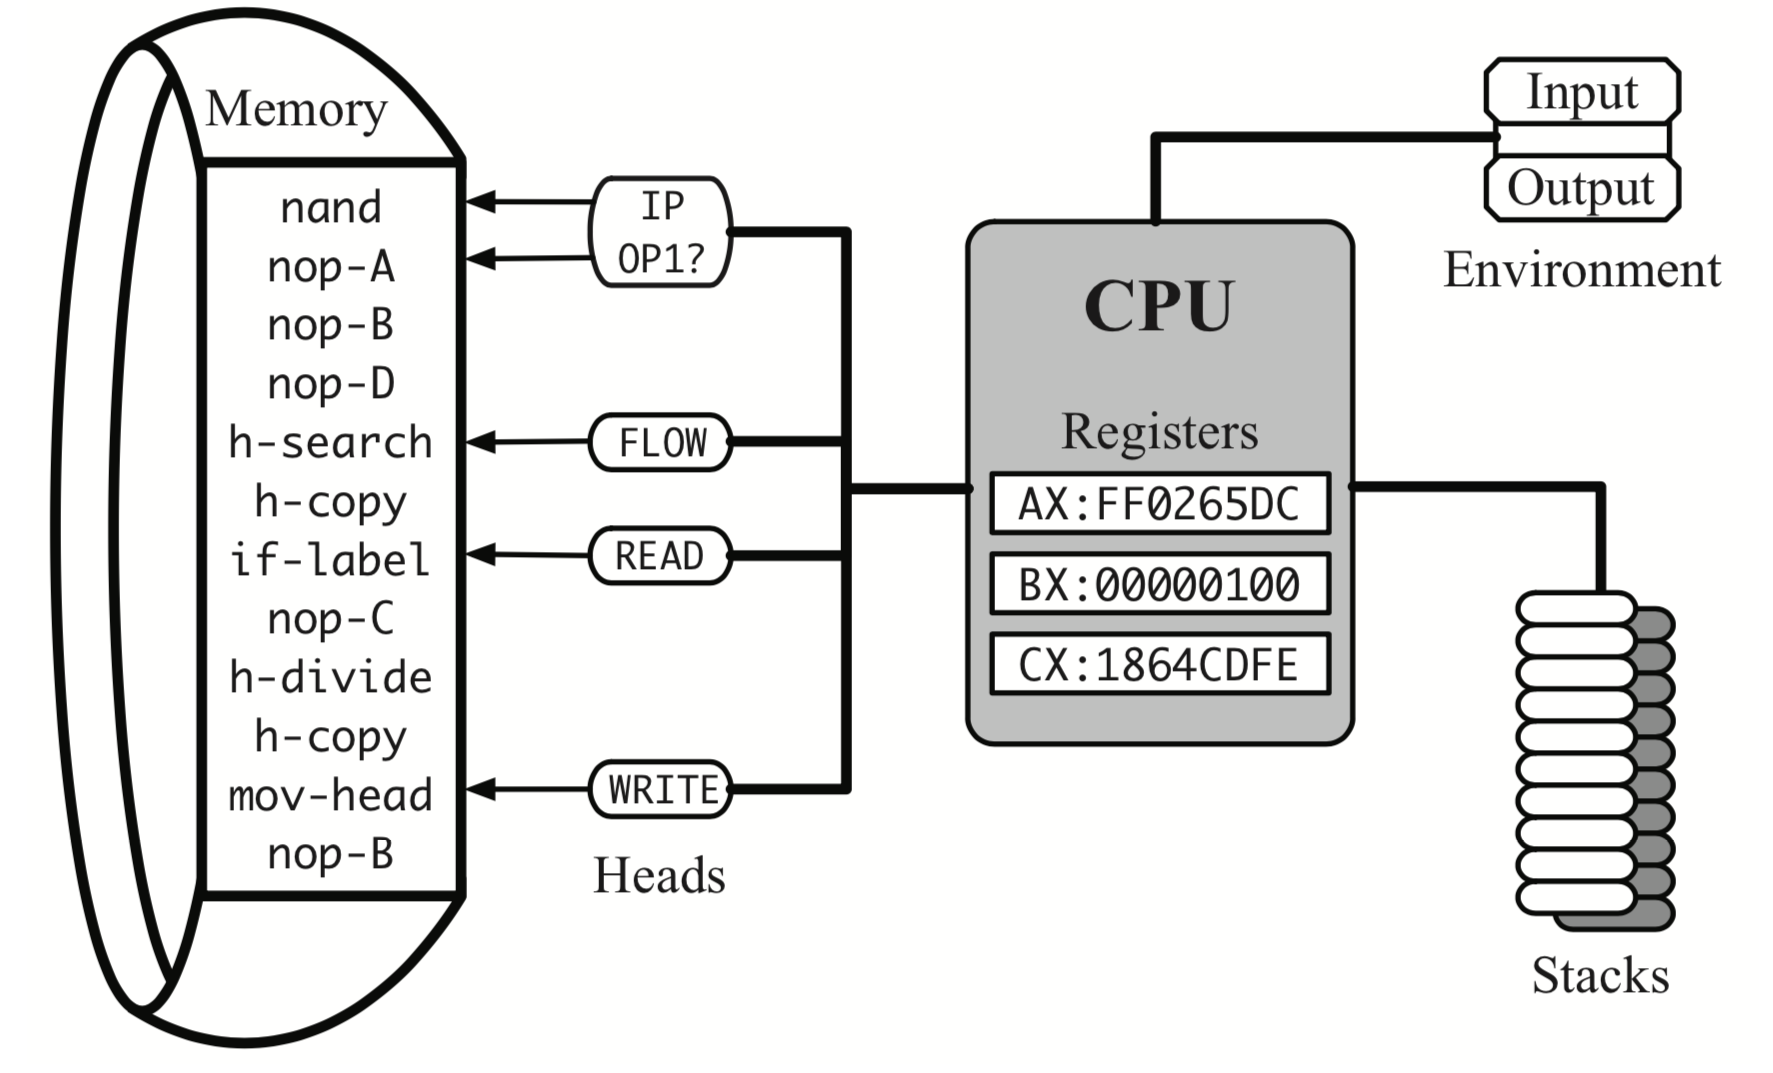
\includegraphics[width=\textwidth]{chapters/02-evolutionary-origins-of-plasticity/media/avida-virtual-cpu.png}
  \caption{\small 
    \textbf{A visual representation of the default virtual hardware used by organisms in Avida. }
    Original figure from \citep{ofria_avida:_2009}.
  }
  \label{chapter:origins-of-plasticity:fig:avida-virtual-cpu}
\end{figure*}

% Metabolism, competition
Organisms can gain additional CPU cycles by performing tasks---such as mathematical computations---to improve their metabolic rate. 
An organism's metabolic rate determines how rapidly it can execute its genome; a higher metabolic rate allows an organism to replicate faster. 
Initially, an organism's metabolic rate is roughly proportional to its genome length; however, the organism's metabolic rate can be adjusted when the organism completes a task. 
In this way, we can differentially reward or punish the performance of different tasks.

When an organism successfully replicates, its offspring is placed in a random location in the world, replacing the organism formerly occupying that location. 
In this way, becoming a more efficient replicator in Avida is advantageous in the competition for space. 
The combination of competition for replication efficiency and heritable variation due to imperfect copying during the replication process results in evolution by natural selection. 

\subsubsection{Sensing in Avida}
\label{chapter:origins-of-plasticity:sec:methods:avida:sensing}

% Sensing in Avida
In a typical Avida run, organisms must execute an instruction called \code{IO} to output the result of a computation. 
That output is analyzed to determine if any tasks have been performed, and if so, the organism is appropriately rewarded or punished. 
However, in this default scenario, organisms cannot sense the result, even after the task has been performed. 
To provide organisms with a mechanism to sense their environment, we added an \code{IO-Sense} instruction to the set of available instructions\footnote{
\code{IO-Sense} is based on the \code{IO-Feedback} instruction implemented in \citep{clune_investigating_2007}, which worked exactly as the default \code{IO} instruction, but provided the organism with feedback on the result.
As such, an organism must first do a particular task once---and potentially get punished---to sense whether or not the task is beneficial with the \code{IO-Feedback} instruction.
}.

The \code{IO-Sense} instruction simulates \code{IO} and provides the organism with feedback on what would have happened if the organism had executed an \code{IO} instruction instead. 
This separation of \code{IO} performance and sensing allows organisms to determine whether or not a particular task is being punished without the risk of punishment, lowering the potential cost of sensing. 
If an \code{IO} operation would have resulted in a punishment, a -1 is added to the top of the organism's stack memory; if it would have resulted in a reward, a 1 is placed there. 
If an \code{IO} operation would have resulted in neither a reward nor a punishment, a 0 is placed on the organism's stack memory. 
In this way, organisms can sense whether or not a particular task is being rewarded or punished in their current environment and then react accordingly.  

\subsubsection{Identifying Phenotypic Plasticity in Avida}
\label{chapter:origins-of-plasticity:sec:methods:avida:identifying-plasticity}

% identifying phenotypic plasticity in avida 
We define a phenotypically plastic organism in Avida as an organism that leverages sensory information to alter their phenotype based on the environment.
We restrict the definition of an organism's phenotype to the set of unique tasks it performs in the given environment. 
We do not consider how many times an organism performs a particular task in a given environment, but only whether the organism does the task at all. 
Thus, to be phenotypically plastic, an organism must express a different task profile (\textit{i.e.}, perform different tasks) in different environments. 

\subsection{Experimental Design}
\label{chapter:origins-of-plasticity:sec:methods:experimental-design}

% Lead-in
To explore the evolutionary history of phenotypically plastic organisms, we used an experimental design based on \citep{clune_investigating_2007}. 

% Environment
\subsubsection{Environments}
\label{chapter:origins-of-plasticity:sec:methods:experimental-design:environments}

We constructed two experimental environments named ENV-NAND and ENV-NOT.
In ENV-NAND, organisms were rewarded for performing the NAND logical task but were punished for performing the NOT logical task. 
Conversely, in ENV-NOT, organisms were rewarded for performing the NOT logical task but were punished for performing the NAND logical task. 
In each of our experimental treatments, we cycled between these two environmental conditions. 
In this way, genotypes with the capacity to sense the current environment and express the appropriate task had a competitive advantage over non-plastic organisms. 

\subsubsection{Phenotypes}
\label{chapter:origins-of-plasticity:sec:methods:experimental-design:phenotypes}

% Possible phenotypes
Given our simple definition of a phenotype, there are only four possible phenotypes in each of the two previously described environments: 
(1) perform only NAND, 
(2) perform only NOT, 
(3) perform both NAND and NOT, 
and (4) perform neither NAND nor NOT. 
When considering an organism's phenotype across both ENV-NAND and ENV-NOT, there are sixteen possible combinations. 
We enumerate these phenotypes in Figure \ref{chapter:origins-of-plasticity:fig:task-profiles}. 
Of these sixteen possible phenotypes, only four express the identical task profile in both environments; the other twelve profiles all exhibit some form of plasticity. 
The optimal form of plasticity is to perform only the NAND task in ENV-NAND and to perform only the NOT task in ENV-NOT; any other form of plasticity is sub-optimal. 
There are five possible phenotypes that leverage plasticity to perform punished tasks instead of rewarded tasks in a given environment; we did not expect these forms of phenotypic plasticity to be successful. 


% Table that enumerates possible phenotypic states
\begin{figure*}[!ht]
  \centering 
  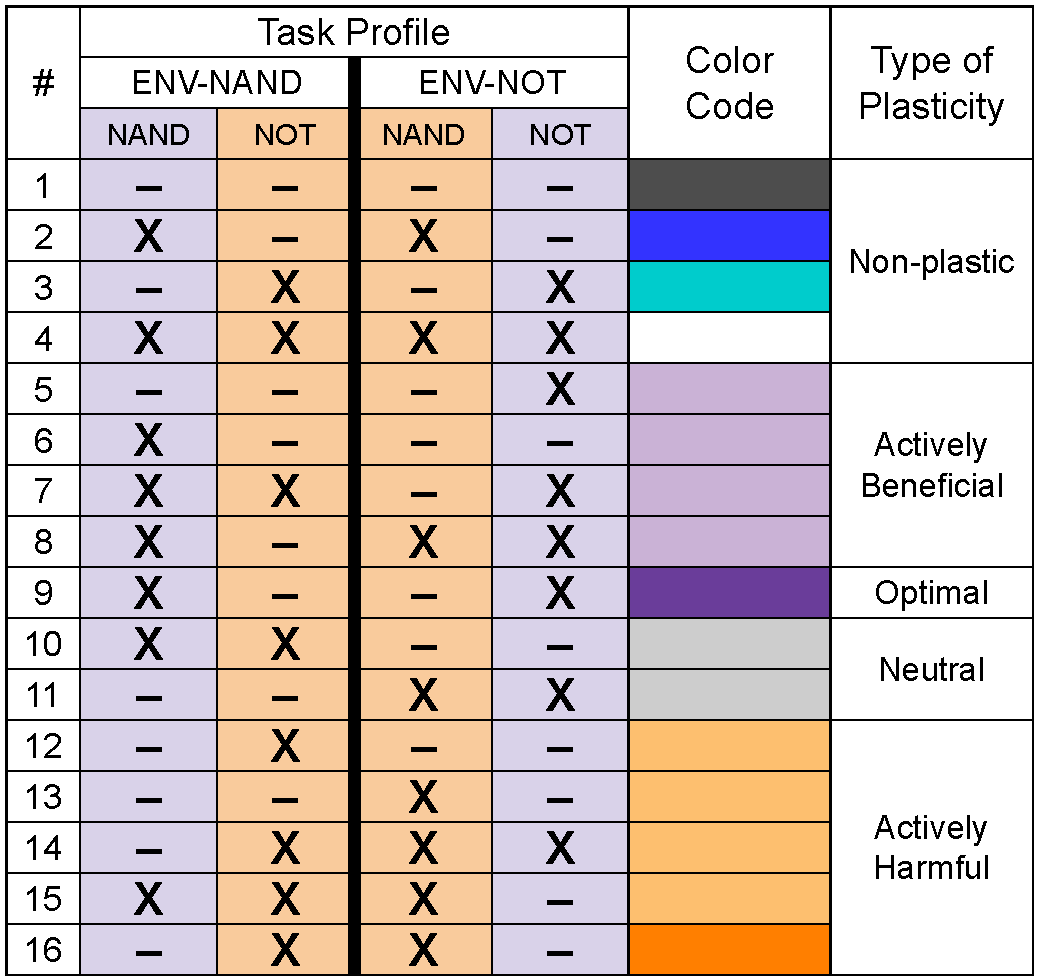
\includegraphics[width=0.75\columnwidth]{chapters/02-evolutionary-origins-of-plasticity/media/task-profiles.pdf}
  \caption{\small 
  \textbf{Enumeration of all possible complete phenotypes.}
  Each row represents a distinct phenotype. 
  An `X' indicates that the associated task is performed in the specified environment, while a `--' indicates that the task is not performed. 
  For each environment, the column of the rewarded task is highlighted in light purple, and the column of the punished task is highlighted in light orange. 
  An `X' in a reward column or a `--' in the punished column is optimal. 
  Each phenotype has a color code, which is used in our lineage visualization visualizations.  
  Note that the first four rows are non-plastic phenotypes, rows 5--8 exhibit partially beneficial plasticity, and row 9 is optimally beneficial.  
  Rows 10--11 are neutral non-adaptive plasticity, while rows 12--16 are detrimental forms of plasticity.}
  \label{chapter:origins-of-plasticity:fig:task-profiles}
\end{figure*}

\subsubsection{Treatments}
\label{chapter:origins-of-plasticity:sec:methods:experimental-design:treatments}

% Experimental treatments
Our experimental design consisted of five treatments and a control: 
(1) a baseline treatment with a moderate point-mutation rate and environmental-cycle length, 
(2) a low-mutation-rate treatment, 
(3) a high-mutation-rate treatment, 
(4) a short-environment-cycle-length treatment, 
(5) a long-environment-cycle-length treatment, 
and (6) a control where both NAND and NOT were rewarded and the environment did not fluctuate. 
See Table \ref{chapter:origins-of-plasticity:table:treatments} for treatment details.

We created the baseline treatment to produce phenotypically plastic organisms for lineage analysis. 
We limited the population size to 3600 organisms and seeded the world with an ancestral genotype capable only of self-replication.
We then evolved populations for 100,000 updates\footnote{
An update in Avida is an experimental length of time. One update is defined as the amount of time it takes for the average organism to execute 30 instructions (see \citep{ofria_avida:_2009} for more details).
} in Avida. 
We imposed a 0.0075 probability of point-mutation per instruction copied, as well as a 0.05 probability for each of single-instruction insertion and deletion per genome copied. 
We fluctuated the current environment between ENV-NAND and ENV-NOT every 100 updates in the baseline treatment. 
We ran 50 replicates of each treatment, including the control. 

% Table 'bout treatments
\begin{table}
\renewcommand{\arraystretch}{1.5}
  \centering
  \small
  \begin{tabular}{| >{\raggedright} p{0.3\columnwidth} |r | r| }
    \hline
    \centering \textbf{Treatment} & \multicolumn{1}{>{\raggedright\arraybackslash}p{0.25\columnwidth}|}{\centering \textbf{Point-mutation Rate}} & \multicolumn{1}{>{\raggedright\arraybackslash}p{0.30\columnwidth}|}{\centering \textbf{Environment Cycle Length }}
    \\ \hline 
    Baseline &  0.0075 &  100 updates  
    \\ \hline 
    Low Mutation Rate &  0.0025 & 100 updates 
    \\ \hline 
    High Mutation Rate &  0.0125 &  100 updates 
    \\ \hline
    Short Environment Cycle Length & 0.0075 &  50 updates 
    \\ \hline 
    Long Environment Cycle Length & 0.0075 &  200 updates 
    \\ \hline 
  \end{tabular}
  \caption{\small 
  \textbf{Differences among the five experimental treatments. }
  Point-mutation rate is given as mutations per instruction copied.
  Environment cycle length describes the length of time (in updates) an environment is active before toggling to the alternative environment.
  }
  \label{chapter:origins-of-plasticity:table:treatments}
\end{table}

\subsubsection{Lineage Visualization}
\label{chapter:origins-of-plasticity:sec:methods:experimental-design:lineage-visualization}

To explore evolutionary strategies evolved in fluctuating environments, we visualized the lineages of evolved genotypes as vertical bars where time (in updates) proceeds from top to bottom beginning with the lineage's original ancestor genotype.
Any given genotype on the lineage must express one of the sixteen possible phenotypes enumerated in Figure \ref{chapter:origins-of-plasticity:fig:task-profiles}.
At each point in time, the color of the visualized lineage corresponds to the color representing the phenotype expressed by the lineage at that point in time. 
For example, because the ancestral organism is capable only of self-replication, all visualized lineages should show that the original ancestor's phenotype performed neither the NAND task nor the NOT task. 
In addition to the visualized lineages, we indicate the actual environmental conditions experienced by the evolving populations at each point in time by the color of the vertical axis. 
This type of visualization allows us to display the phenotypic states traversed by any given lineage, allowing us to explore evolutionary strategies leveraged by all evolved lineages.

\section{Results and Discussion}

\subsection{What conditions promote the evolution of phenotypic plasticity?}

Ghalambor \textit{et al.} identified four environmentally-dependent requirements for the evolution of phenotypic plasticity
\citep{ghalambor_behavior_2010}. 
Our experimental design conforms to these conditions, enabling us to test their validity and relative importance. 
The oscillation between ENV-NAND and ENV-NOT provides temporal variation. 
The IO-Sense instruction reliably indicates the current environment. 
The two environments favor opposing phenotypic traits, and the only way for an individual organism to achieve a high fitness in both environments is to alter its phenotypic expression. 
Given the existing theoretical and empirical support for these conditions, we expected to see the evolution of phenotypic plasticity in each of our experimental treatments. 
However, we were unsure of the impact of altering environmental factors such as mutation rate and environment fluctuation rate. 

% Report plasticity results. 
At the end of the experiment, we extracted the dominant (most abundant) genotype from the population of each replicate.
We tested these genotypes in both ENV-NAND and ENV-NOT and recorded each genotype's expressed phenotype across both environments. 
In Table \ref{chapter:origins-of-plasticity:table:evolutionary-outcomes}, we report the number of replicates in which the dominant genotype at the end of the experiment was plastic and the number of replicates in which the dominant genotype was optimally plastic. 
Note that for these results we only evaluated the most abundant genotype at the end of the experiment. 
An ancestor of the evaluated genotype may have been plastic, but if that plasticity was not maintained in the lineage, we did not count it in Table \ref{chapter:origins-of-plasticity:table:evolutionary-outcomes}. 

% More specifically report results
As expected, the capacity for phenotypic plasticity evolved in each experimental treatment; in 31 of the 50 baseline treatment replicates, phenotypic plasticity was present in the final dominant organism. 
None of the final dominant genotypes from the control replicates were phenotypically plastic. 
In all control replicates, the dominant genotype performed both the NAND and NOT tasks unconditionally. 
Our results are consistent with existing theoretical and empirical work, supporting the validity of the conditions likely to facilitate the evolution of phenotypic plasticity \citep{clune_investigating_2007,ghalambor_behavior_2010,hallsson_selection_2012,nolfi_phenotypic_1994}. 

\begin{table*}[t]
\renewcommand{\arraystretch}{1.5}
	\centering
    \small
    \begin{tabulary}{\textwidth}{| l | r | r | r | r | r |}
      \hline 
      \multicolumn{1}{| c |}{\centering \textbf{Treatment}} &
      \multicolumn{2}{ c |}{\centering \textbf{Plastic Replicates}} &
      \multicolumn{2}{ p{0.25\textwidth}|}{\centering \textbf{Unconditional Precedes Conditional}} & \multicolumn{1}{p{0.20\textwidth}|}{\centering \textbf{Sub-optimal Precedes Optimal}} \\
      \cline{2-5}
      & \multicolumn{1}{p{0.1\textwidth} |}{\centering Total} & \multicolumn{1}{p{0.1\textwidth} |}{\centering Optimal$^{*}$} & \multicolumn{1}{p{0.1\textwidth} |}{\centering NAND Task} & \multicolumn{1}{p{0.1\textwidth} |}{\centering NOT Task} & \\
      \hline 
      Baseline 						 & 31 (62\%) & 17 (34\%) & 31 (100\%)   & 28 (90.3\%) & 16 (94.1\%) \\
      \hline 
      Low Mutation Rate 			 & 38 (76\%) & 30  (60\%) & 34 (89.5\%) & 35 (92.1\%) & 30 (100\%) \\
      \hline 
      High Mutation Rate  			 & 25 (50\%) & 11  (22\%) & 25 (100\%)  & 24 (96\%)  & 10 (90.9\%) \\
      \hline 
      \parbox[t]{0.2\textwidth}{Short Environment Cycle Length} & 36 (72\%) & 18  (36\%) & 33 (91.7\%) & 28 (77.8\%) & 18 (100\%) \\
      \hline 
      \parbox[t]{0.2\textwidth}{Long Environment Cycle Length}  & 16 (32\%) & 10  (20\%) & 14 (87.5\%) & 16 (100\%)  & 9 (90\%) \\
      \hline 
      Control						 & 0 (0\%) & 0 (0\%) & \multicolumn{1}{c|}{--} & \multicolumn{1}{c|}{--} & \multicolumn{1}{c|}{--} \\
      \hline 
    \end{tabulary}
    \begin{tablenotes}
          \item[*] $^{*}$\small{Optimal is defined as the complete phenotype that only performs the rewarded task in each environment.}
    \end{tablenotes}
    \caption{\small 
    \textbf{A summary of evolutionary outcomes across all five experimental treatments and control.}
    Plastic Replicates indicates the number of replicates (out of 50 per treatments) in which the final dominant genotype was plastic at all (Total) and perfectly plastic (Optimal).  
    Unconditional Precedes Conditional indicates the number of times the NAND task and NOT task were expressed unconditionally before eventually evolving to be express conditionally (out of total plastic).  
    Finally, Sub-optimal Precedes Optimal indicates how many runs had an imperfect form of plasticity before eventually evolving to be optimally plastic (out of total optimally plastic).
    }
    \label{chapter:origins-of-plasticity:table:evolutionary-outcomes}
\end{table*}

\subsection{How do environmental factors impact the evolution of phenotypic plasticity?}

While our results show phenotypic plasticity can evolve under the conditions identified in \citep{ghalambor_behavior_2010}, how do mutation rate and fluctuation rate affect the evolution of phenotypic plasticity under these conditions? 
We found compelling results for both mutation rate and environmental cycle length. 

\subsubsection{Mutation Rate}

While only of borderline statistical significance ($p = 0.058$ using Fisher's Exact Test with Bonferroni corrections for multiple comparisons; all statistics were done in R version 3.2.2 \citep{r_core_team_2016}), our results trend such that populations at lower mutation rates appear more likely to evolve phenotypic plasticity than do populations at higher mutation rates. 
The most abundant genotypes exhibited some plasticity in 38/50 runs at a low mutation rate, 31/50 at the baseline mutation rate, and 25/50 and the high mutation rate.  
While higher mutation rates increase genetic variation from one generation to the next, most mutations that have phenotypic effects are deleterious \citep{sniegowski_evolution_2000}. 
Thus, at higher mutation rates, the elevated influx of deleterious mutations could increase the difficulty of maintaining the necessary genetic machinery for phenotypic plasticity.
Qualitative evidence for this effect can be seen in the time-sliced visualized lineages of final dominant, non-plastic genotypes from the high-mutation-rate treatment (Figure \ref{chapter:origins-of-plasticity:fig:high-mut-lineages}) where lineages traverse states of plasticity for some time before reverting back to states of non-plasticity\footnote{
For fully interactive visualizations of evolved lineages from all treatments, see \url{https://lalejini.com/evo-origins-of-phenotypic-plasticity-web/}
}.
Furthermore, more phenotypic shifts in general increase the probability of quickly finding an appropriate non-plastic phenotype after each environmental change.

\begin{figure*}[ht]
  \centering
  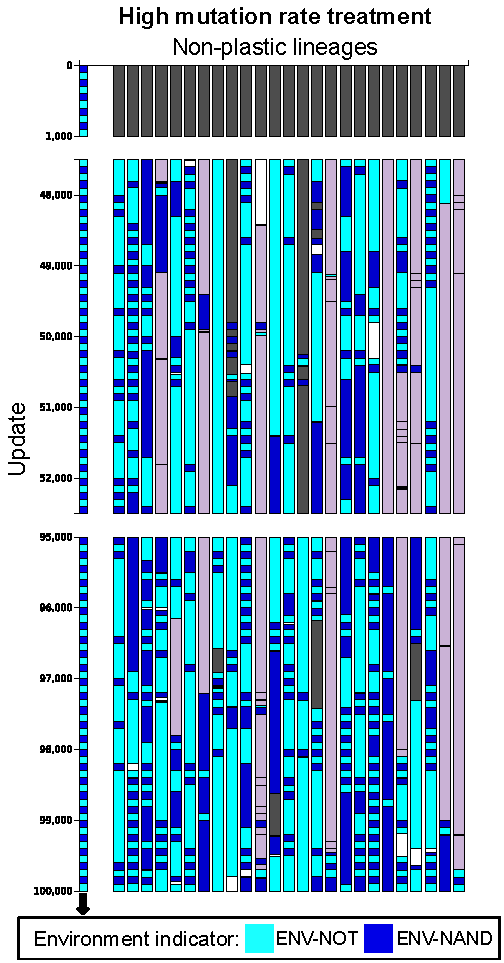
\includegraphics[height=0.5\textheight, keepaspectratio]{chapters/02-evolutionary-origins-of-plasticity/media/high-mutation-rate-non-plastic-lineages.pdf}
  \caption{\small 
  \textbf{Time-sliced visualization of lineages for non-plastic, dominant genotypes from the high-mutation-rate treatment.}
  Abbreviated color reference: 
  cyan represents unconditional NOT task performance, 
  dark blue represents unconditional NAND task performance, 
  and light purple represents sub-optimal forms of plasticity.  
  Refer to Figure \ref{chapter:origins-of-plasticity:fig:task-profiles} for a full legend of phenotype colors.}
  \label{chapter:origins-of-plasticity:fig:high-mut-lineages}
\end{figure*}



% Plastic lineages from the baseline treatment
\begin{figure*}[!ht]
  \centering
  \begin{minipage}[b]{\linewidth}
  \centering
  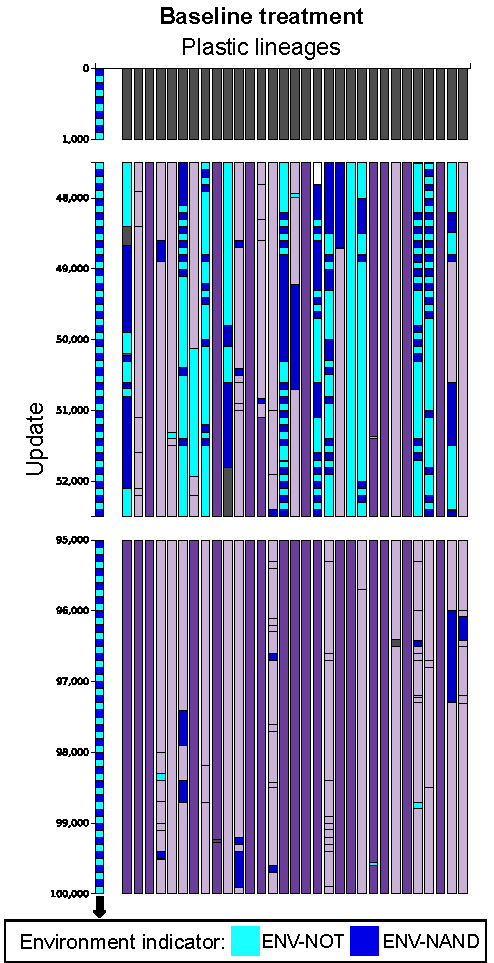
\includegraphics[height=0.5\textheight, keepaspectratio]{chapters/02-evolutionary-origins-of-plasticity/media/baseline-plastic-lineages.pdf}
  \caption{\small 
  Time-sliced lineage visualization of dominant, plastic genotypes from the baseline treatment. 
  Abbreviated color reference: 
  cyan represents unconditional NOT task performance, 
  dark blue represents unconditional NAND task performance, 
  light purple represents sub-optimal forms of plasticity, 
  and dark purple represents optimal plasticity.  
  Refer to Figure \ref{chapter:origins-of-plasticity:fig:task-profiles} for a full legend of phenotype colors.}
  \label{chapter:origins-of-plasticity:fig:baseline-lineages}
  \end{minipage}
\end{figure*}

\subsubsection{Environment Fluctuation Rate}

We found a significant difference ($p = 0.00028$ using Fisher's Exact Test with Bonferroni corrections for multiple comparisons) as we varied the cycle length for environmental switching.  
Specifically, in the long-environment-cycle-length, only 16/50 runs ended with a final dominant genotype that was phenotypically plastic, while the baseline and short-environment-cycle-length produced 31 and 36 plastic outcomes, respectively.

We expect that the short-environment-cycle-length treatment is biased toward the evolution of phenotypic plasticity because of the rapid environment fluctuations relative to other experimental treatments. 
Rapid fluctuations cause lineages to be less able to rely on mutational input for adaptation. 
In the long-environment-cycle-length treatment, environmental fluctuations may not occur rapidly enough to produce a sufficient selective pressure for phenotypic plasticity, allowing alternative adaptive strategies to evolve instead.

\subsection{What are the evolutionary stepping stones for phenotypic plasticity?}

In an attempt to identify patterns frequently encountered during the evolution of phenotypically plastic organisms, we extracted and analyzed the full lineages from our experiments. 
We tested each ancestor genotype in both ENV-NAND and ENV-NOT and classified their phenotype across both environments. 
In addition to a quantitative analysis, we also visualized the lineages of the dominant, plastic genotypes; see Figure \ref{chapter:origins-of-plasticity:fig:baseline-lineages} for the visualization of the baseline treatment. 
Using our visualizations and ancestor phenotype classifications, we addressed the following two questions: 
(1) Do the lineages of phenotypically plastic organisms first evolve to perform tasks unconditionally before evolving to perform them conditionally as a function of their current environment? 
And (2), do imperfect forms of phenotypic plasticity tend to precede optimal forms?

\subsubsection{Unconditional task performance precedes plasticity}

To explore whether or not unconditional task performance was an evolutionary stepping stone for conditional task performance (\textit{i.e.}, phenotypic plasticity), we determined whether a task was performed unconditionally prior to being performed conditionally by the ancestors of plastic genotypes. 
We analyzed both tasks (NAND and NOT) separately. These results are reported in Table \ref{chapter:origins-of-plasticity:table:evolutionary-outcomes}. 
% Answer to: unconditional before conditional?
Across all experimental treatments, non-plastic ancestors generally preceded plastic ancestors. 
In other words, unconditional task performance of the NAND and NOT tasks generally preceded the conditional performance of either task. 
Examples of this can be seen in time-sliced plastic lineages from the baseline treatment (Figure \ref{chapter:origins-of-plasticity:fig:baseline-lineages}) where many lineages maintain states of unconditional task expression prior to entering states of conditional task expression. 
These results suggest that, in fluctuating environments similar to those in our experiment, the evolutionary path to phenotypic plasticity usually traverses states of unconditional trait expression prior to entering states of conditional trait expression. 
This result should be unsurprising. 
In order to evolve a regulated function, the capacity for both the regulation and the function must exist. 
In our experiment, the function can be selected for without regulation; however, regulation of the function is unlikely to be selected for without the prior capacity for the function. 

\subsubsection{Sub-optimal plasticity precedes optimal plasticity}

To investigate sub-optimal phenotypic plasticity as an evolutionary stepping stone for optimal phenotypic plasticity in our experiment, we analyzed lineages of optimally plastic genotypes. 
Again, we consider only complete phenotypes that exclusively perform the rewarded task in each environment to be optimal. 
For each optimally plastic genotype's lineage, we determined whether or not the evolution of optimal plasticity was preceded by the evolution of sub-optimal phenotypic plasticity. 
The results of this analysis are reported in Table \ref{chapter:origins-of-plasticity:table:evolutionary-outcomes}.

% Answer to: sub-optimal before optimal?
Across all experimental treatments, the evolution of sub-optimal plasticity did, indeed, generally precede the evolution of optimal phenotypic plasticity.
Examples of sub-optimal plasticity preceding more optimal forms of plasticity can be seen in some of the time-sliced lineages from the baseline treatment visualized in Figure \ref{chapter:origins-of-plasticity:fig:baseline-lineages}. 
These results suggest that, in fluctuating environments similar to those in our experiment, sub-optimal forms of phenotypic plasticity tend to arise before the evolution of optimal forms of phenotypic plasticity. 

Unconditional trait expression tends to evolve first; then, sub-optimal forms of plasticity appear before optimal forms finally evolve.
While challenging to verify, we expect our results to be applicable to biological systems. 
The evolution of complex functions (\textit{e.g.}, optimal phenotypic plasticity) build on simpler, previously evolved functions (\textit{e.g.}, unregulated or sub-optimally regulated functions) \citep{lenski_evolutionary_2003}. 
These results, however, are particularly useful for applied evolutionary computation. 
If an evolved problem solution must respond dynamically to environmental variables, it is likely that the solution will need to be able to traverse through states of rigidity and sub-optimal plasticity prior to reaching a state of optimal plasticity. 
Thus, first evolving rigid solutions in fixed environments and then gradually starting to fluctuate more aspects of the environment over time could provide a scaffolding for the evolution of optimally plastic solutions.  

\subsection{Does plasticity still evolve when evolutionary stepping stones are disallowed?}

% Describe experiment
% - To investigate the importance of each of our observed stepping stones (unconditional trait expression and sub-optimal plasticity), we conducted a followup set of experiments.
We conducted a series of followup experiments to investigate the importance of unconditional trait expression and sub-optimal plasticity as evolutionary stepping stones.
We evolved 200 replicate populations under baseline treatment conditions (described in Section \ref{chapter:origins-of-plasticity:sec:methods:experimental-design}) and 200 replicate populations in each of three experimental conditions where we disallowed particular phenotypic profiles from evolving: (1) we disallowed phenotypes that expressed NAND and/or NOT unconditionally (\textit{i.e.}, task profiles 2, 3, and 4 from Figure \ref{chapter:origins-of-plasticity:fig:task-profiles}); (2) we disallowed sub-optimally plastic phenotypes (\textit{i.e.}, task profiles 5 through 8 and 10 through 16 from Figure \ref{chapter:origins-of-plasticity:fig:task-profiles}); and, (3) we disallowed phenotypes that exhibited unconditional trait expression \textit{or} phenotypes that were sub-optimally plastic (\textit{i.e.}, all task profiles except 1 and 9 from Figure \ref{chapter:origins-of-plasticity:fig:task-profiles}).
Note that in each of these experimental treatments, we always allowed phenotypes that expressed no tasks or were optimally plastic across both environments.
In treatments where particular phenotypes were disallowed, we tested all offspring in both ENV-NAND and ENV-NOT; if the phenotype of an organism's offspring was among the disallowed phenotypes, we prevented its birth.
As in our previous experiments, we counted the number of replicates of each treatment where the dominant genotype at the end of the experiment exhibited a plastic phenotype.
% @AML: should give each experimental treatment a name (e.g., no-unconditional-expression, no-sub-optimal-plasticity, and no-intermediate-phenotypes)

\begin{figure*}[!ht]
  \centering
  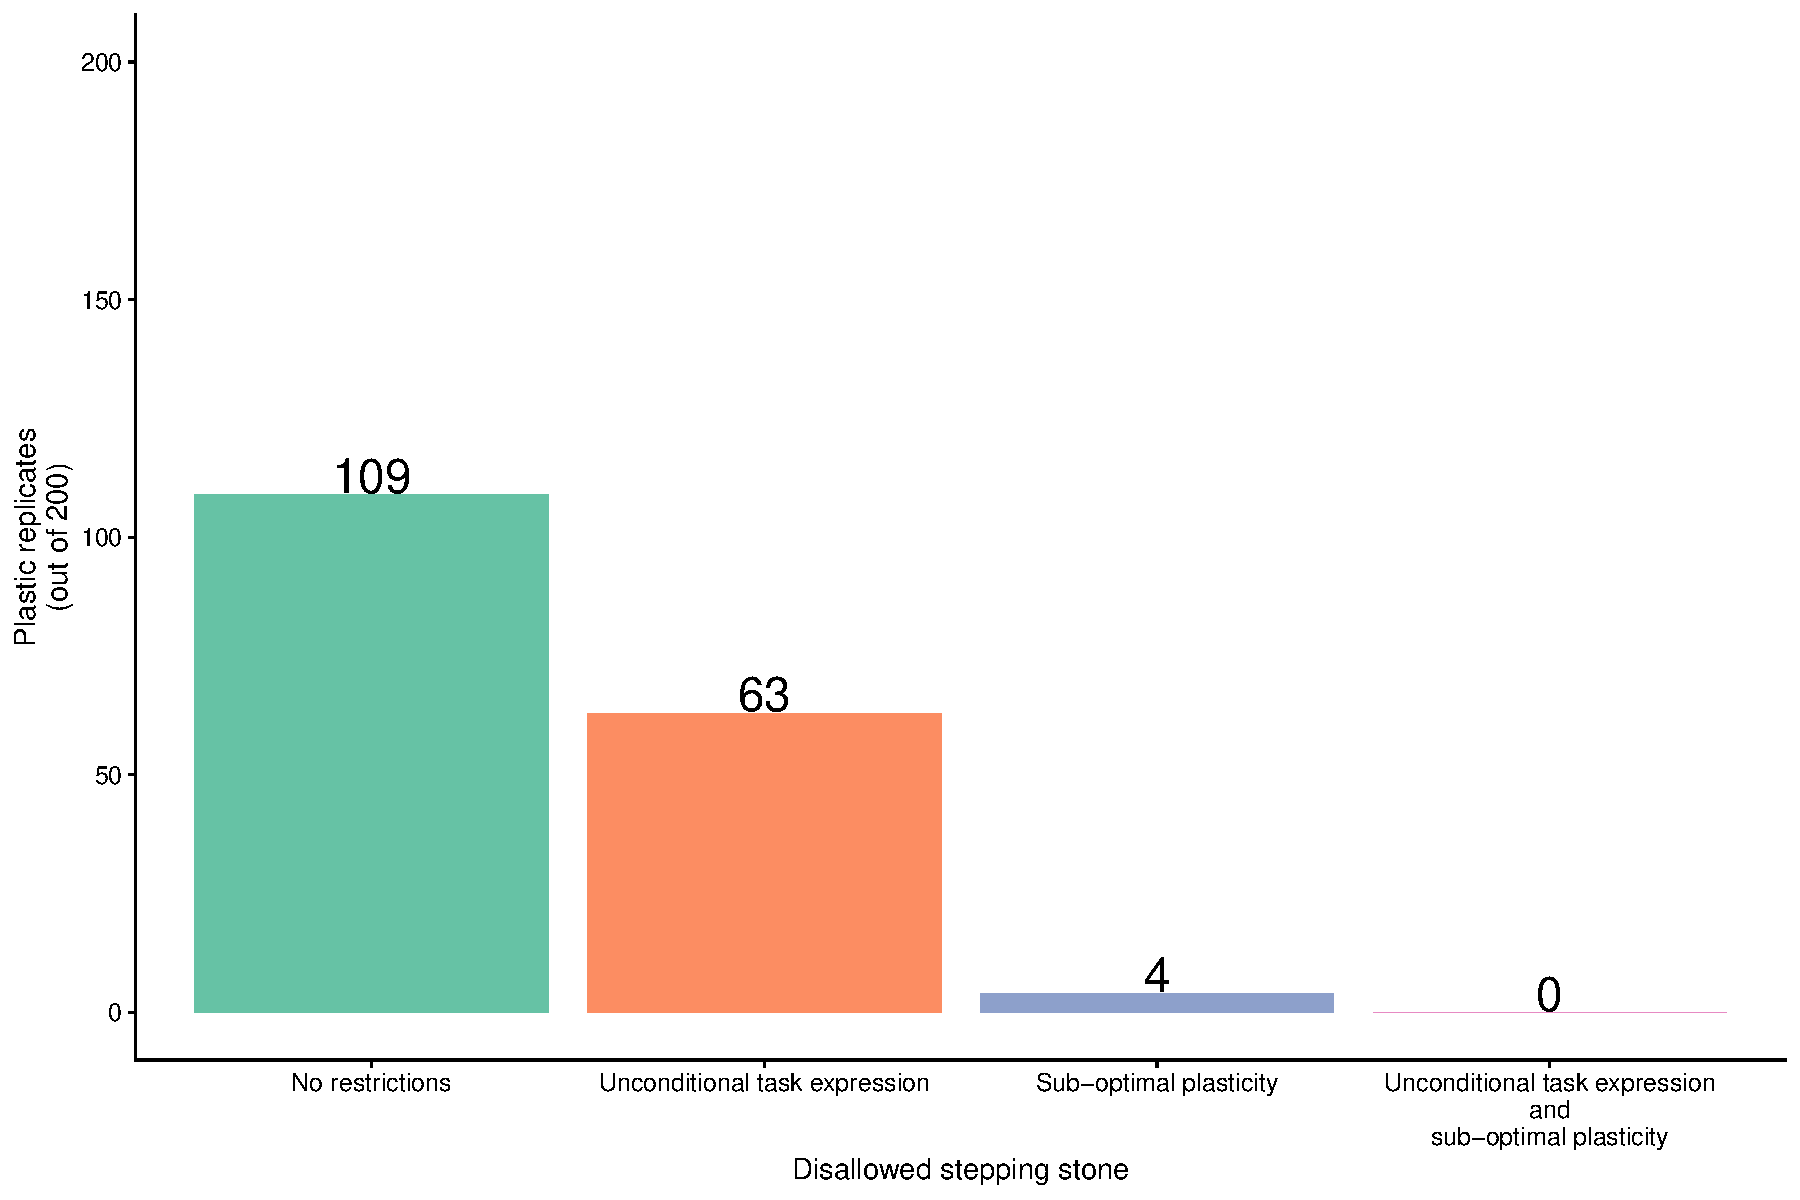
\includegraphics[height=0.3\textheight, keepaspectratio]
  {chapters/02-evolutionary-origins-of-plasticity/media/blocked-stepping-stones-baseline.pdf}
  \caption{\small A summary of evolutionary outcomes. 
  For each condition, the bar plot indicates the number of replicates (out of 200 per condition) where the final dominant genotype was plastic.
  }
  \label{chapter:origins-of-plasticity:fig:blocked-stepping-stones}
\end{figure*}

% Describe results
Figure \ref{chapter:origins-of-plasticity:fig:blocked-stepping-stones} gives the number of plastic replicates that evolved in each experimental condition.
We compared each of the three treatments that disallowed stepping stone phenotypes to our unmodified baseline treatment (Fisher's exact test with a significance level of 0.05 and a Bonferonni correction for multiple comparisons).
Each of the three treatments where we disallowed offspring with particular phenotypes had significantly fewer replicates with a plastic dominant genotype at the end of the experiment (unconditional trait expression disallowed: $p<10^{-4}$; sub-optimal plasticity disallowed: $p<10^{-4}$; both unconditional trait expression and sub-optimal plasticity disallowed: $p<10^{-4}$).

% -- Discuss --
% No intermediate phenotypes => no plasticity evolves
No phenotypically plastic genotypes evolved when we disallowed all intermediate phenotypes; when all intermediate phenotypes were disallowed, only two phenotypes were possible: (1) performing neither the NOT nor NAND tasks across environments and (2) optimally regulating between the NOT and NAND tasks across environments.
For plasticity to evolve without allowing evolution to traverse intermediate stepping stones, optimal plasticity would need arise in a single mutational step from a genotype that performed neither the NAND nor NOT tasks.
This result demonstrates that, together, these intermediate phenotypes represent crucial building blocks for the evolution of phenotypic plasticity. 

% No unconditional task expression => less plasticity
% No sub-optimal plasticity => even less plasticity
When we prevented genotypes that perform tasks unconditionally across environments, plasticity evolved less frequently than in treatments where we placed no restrictions on phenotypes; this supports our previous observation that unconditional task expression is a stepping stone toward plastic task expression. However, many replicates (63 out of 200) where unconditional task expression was disallowed still yielded plastic organisms. Thus, while unconditional trait expression is likely a valuable building block in the evolution of phenotypic plasticity, it is not necessary. Our results indicate that sub-optimal plasticity is a more important building block for optimal plasticity than unconditional trait expression. Only 4 out of 200 replicates where we disallowed sub-optimally plastic phenotypes yielded optimal plasticity. This is not unsurprising, as a lineage would need to move from a state of unconditional task expression to perfect task regulation in a single mutational step.

\subsection{Are stochastic strategies evolving as an alternative to phenotypic plasticity?}

Stochastic phenotype switching, a form of bet hedging \citep{seger_what_1987}, is a common strategy leveraged by bacteria in fluctuating environments \citep{rainey_evolutionary_2011}. 
Some forms of stochastic phenotype switching rely on mutational input to induce phenotypic changes. 
This strategy is thought to be a viable alternative to phenotypic plasticity in the absence of reliable environmental signals or when the processing of sensory information is costly \citep{rainey_evolutionary_2011}.
Strategic stochastic phenotype switching often relies on contingency loci, which are hypermutable regions of the genome that can induce phenotype switching via mutational input \citep{moxon_bacterial_2006}. 

We hypothesized that stochastic phenotype switching was an alternative evolutionary strategy to phenotypic plasticity because of its commonality in bacteria. 
We most expected to see stochastic phenotype switching in our experimental treatments where the fewest number of replicates produced phenotypically plastic final dominant genotypes. 

\subsubsection{Lineage Visualization}

It can be difficult to intuitively understand evolutionary strategies leveraged by a lineage without a visual aid.
To explore evolutionary strategies alternative to phenotypic plasticity in fluctuating environments, we visualized the lineages of dominant, non-plastic genotypes from our experimental treatments. 

\begin{figure*}[ht!]
  \centering
  \begin{minipage}[b]{\linewidth}
  \centering
  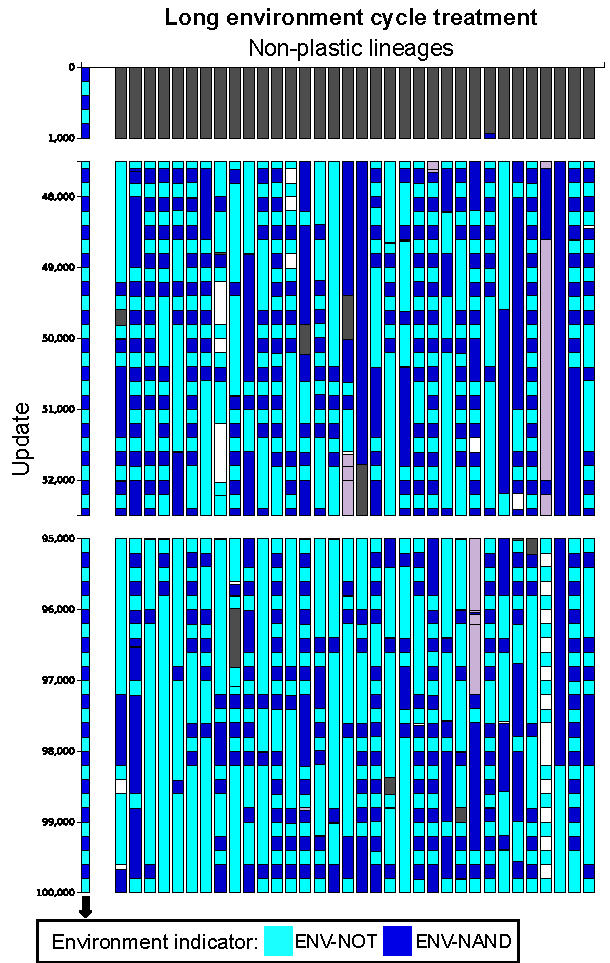
\includegraphics[height=0.4\textheight, keepaspectratio]
  {chapters/02-evolutionary-origins-of-plasticity/media/long-cycle-non-plastic-lineages.pdf}
  \caption{\small 
  Time-sliced lineage visualization of non-plastic, dominant genotypes from the long environment cycle treatment. 
  Abbreviated color reference: 
  cyan represents unconditional NOT task performance, 
  dark blue represents unconditional NAND task performance, 
  light purple represents sub-optimal forms of plasticity,
  and dark purple represents optimal plasticity. 
  Refer to Figure \ref{chapter:origins-of-plasticity:fig:task-profiles} for a full legend of phenotype colors.
  }
  \label{chapter:origins-of-plasticity:fig:long-cycle-lineages}
  \end{minipage}
\end{figure*}


If a lineage relied on stochastic phenotype switching, we would expect it to switch between phenotypic states of unconditional NAND task performance and unconditional NOT task performance in approximate synchronization with the changing environment. 
Specifically, we should see ancestors along a lineage perform NAND unconditionally during periods of ENV-NAND and see ancestors performing NOT unconditionally during periods of ENV-NOT. 
We show a time-sliced lineage visualization of dominant, non-plastic genotypes at the end of our experiment for the long-environment-cycle-length treatment (Figure \ref{chapter:origins-of-plasticity:fig:long-cycle-lineages}).  

From Figure \ref{chapter:origins-of-plasticity:fig:long-cycle-lineages}, we see what appear to be cases of stochastic phenotype switching.
That is, we observe lineages switching between phenotypic states of unconditional NAND task performance and unconditional NOT task performance in approximate synchronization with the environment. 
Many of the lineages in the long-environment-cycle treatment seem to be undergoing stochastic phenotype switching. 
A few examples of what appear to be stochastic phenotype switching can even be seen in Figure \ref{chapter:origins-of-plasticity:fig:baseline-lineages} (the plastic lineages from our baseline treatment) between updates 47,500 and 52,500 (the middle time-slice), prompting the following open question: in addition to being an alternative strategy to plasticity in fluctuating environments, could stochastic phenotype switching also act as a precursor or building block toward plasticity? 

Our visualizations only provide an exploratory method for understanding evolutionary strategies employed by a lineage. 
Further analysis would be required to confirm or reject our hypothesis that stochastic phenotype switching is evolving as an alternative strategy to phenotypic plasticity in our system. 
This hypothesis is particularly worthwhile to explore because our mutation rate was fixed across the genome, preventing the evolution of contingency loci.  
Furthermore, because sensing mechanisms were perfectly accurate, phenotypic plasticity was a reliable strategy. 
We hypothesize that genotypes are moving to a region of the mutational landscape that straddles the boundary between expressing unconditional NAND task performance and unconditional NOT task performance such that minimal mutational input is required to switch phenotypes. 
This type of evolutionary trajectory has been demonstrated by Crombach and Hogeweg in evolutionary simulations of simple, genome-encoded gene regulatory network models \citep{crombach_evolution_2008}.
In their simulations, Crombach and Hogeweg found that networks evolved in an oscillating environment possessed genotype to phenotype mappings that were mutationally more efficient at generating adaptive phenotypes in alternative environments. 
\section{Conclusion}

In this work, we evolved populations of phenotypically plastic organisms at varied rates of environmental fluctuation and mutation using the Avida Digital Evolution Platform. 
We analyzed the lineages of evolved genotypes for clues about the evolutionary stepping stones toward phenotypic plasticity. 
We found that the capacity for phenotypic plasticity evolved under conditions identified by previous research \citep{clune_investigating_2007,ghalambor_behavior_2010}. 
We found evidence that traits are generally expressed unconditionally prior to the evolution of conditional trait expression and that sub-optimal forms of phenotypic plasticity generally evolve before optimal forms of phenotypic plasticity. 
Both of these results are examples of evolution's use of simpler functions as building blocks for more complex functions as in~\cite{lenski_evolutionary_2003}. 

Visual inspection of the evolutionary histories leading to phenotypically plastic organisms suggests that under certain conditions stochastic phenotype switching evolves as an alternative strategy to phenotypic plasticity, just as it does in many bacteria \citep{moxon_bacterial_2006,rainey_evolutionary_2011}.  
Of course, in these bacterial cases, hypermutable sites tend to appear in the genomes (called ``contingency loci'') that facilitate such task switching.

Given these promising results, we plan to explore whether stochastic phenotype switching can be a viable evolutionary strategy in the absence of the ability to evolve hypermutable regions of the genome. 
Given the potential difficulty in maintaining the necessary genetic machinery associated with phenotypic plasticity, are there cases in which stochastic phenotype switching is more robust than phenotypic plasticity? 
And, does this contribute to the evolution of stochastic phenotype switching as an evolutionary strategy? 
Metrics are clearly needed for quantifying stochastic phenotype switching in digital systems and for evaluating the mutational landscapes of genotypes along a lineage. 
\chapter{The Evolutionary Consequences of Adaptive Phenotypic Plasticity}
\chapter{Evolving Event-driven Programs with SignalGP}

%%%%%%%%%%%%%%%%%%%%%%%%%%%%%%
% Evolutionary change rate experiment
%%%%%%%%%%%%%%%%%%%%%%%%%%%%%%

% data from experiment - 2021-02-08
\newcommand{\evolutionaryChangeRateReplicates}{100}

\newcommand{\evolutionaryChangeRatePlasticReps}{42}


%%%%%%%%%%%%%%%%%%%%%%%%%%%%%%
% Novel traits experiment
%%%%%%%%%%%%%%%%%%%%%%%%%%%%%%
\newcommand{\novelTraitsReplicates}{100}
\newcommand{\novelTraitsReward}{10\%}
\newcommand{\novelTraitsPlasticReps}{42}

%%%%%%%%%%%%%%%%%%%%%%%%%%%%%%
% Deleterious hitchhiking experiment
%%%%%%%%%%%%%%%%%%%%%%%%%%%%%%
% - 2021-02-05 -
\newcommand{\deleteriousHitchhikingReplicates}{100}
\newcommand{\deleteriousHitchhikingPlasticReps}{43}
\newcommand{\instPoisonMagnitude}{10\%}

\noindent
Authors: Alexander Lalejini and Charles Ofria \\
This chapter is adapted from ~\citep{lalejini_evolving_2018}, which underwent peer review and appeared in the proceedings of the 2018 Genetic and Evolutionary Computation Conference.

\section{Introduction}

% SignalGP exists; we did it!
Here, we introduce SignalGP, a new genetic programming (GP) technique designed to provide evolution direct access to the event-driven programming paradigm, allowing evolved programs to handle signals from the environment or from other agents in a more biologically inspired way than traditional GP approaches. 
In SignalGP, signals (\textit{e.g.}, from the environment or from other agents) direct computation by triggering the execution of program modules (\textit{i.e.}, functions). 
SignalGP augments the tag-based referencing techniques demonstrated by Spector \textit{et al.}
\citep{spector_tag-based_2011,spector_whats_2011,spector_tag-based_2012} to specify which function is triggered by a signal, allowing the relationships between signals and functions to evolve over time. 
The SignalGP implementation presented here is demonstrated in the context of linear GP, wherein programs are represented as linear sequences of instructions; however, the ideas underpinning SignalGP are generalizable across a variety of genetic programming representations. 

% Linear GP is imperative. Event-driven computing is different.
Linear genetic programs generally follow an imperative programming paradigm where computation is driven procedurally.
Execution often starts at the top of a program and proceeds in sequence, instruction-by-instruction, jumping or branching as dictated by executed instructions \citep{brameier_linear_2007,mcdermott_genetic_2015}.
In contrast to the imperative programming paradigm, program execution in event-driven computing is directed primarily by signals (\textit{i.e.}, events), easing the design and development of programs that, much like biological organisms, must react on-the-fly to signals in the environment or from other agents. 
Is it possible to provide similarly useful abstractions to evolution in genetic programming? 

Different types of programs are more or less challenging to evolve depending on how they are represented and interpreted.  
By capturing the event-driven programming paradigm, SignalGP targets problem domains where agent-agent and agent-environment interactions are crucial, such as in robotics or distributed systems. 

In the following sections, we provide a broad overview of the event-driven paradigm, discussing it in the context of an existing event-driven software framework, cell signal transduction, and an evolutionary computation system for evolving robot controllers. 
Next, we discuss our implementation of SignalGP in detail. 
Then, we use SignalGP to demonstrate the value of capturing event-driven programming in GP with two test problems: an environment coordination problem and a distributed leader election problem. 
Finally, we conclude with planned extensions, including how SignalGP can be generalized beyond our linear GP implementation to other forms of GP. 
\section{The event-driven paradigm}

% What is event-driven paradigm?
The event-driven programming paradigm is a software design philosophy where the central focus of development is the processing of events
\citep{etzion_event_2010,heemels_introduction_2012,cassandras_event-driven_2014}. 
Events often represent messages from other agents or processes, sensor readings, or user actions in the context of interactive software applications. 
Events are processed by callback functions (\textit{i.e.}, event-handlers) where the appropriate event-handler is determined by an identifying characteristic associated with the event, often the event's name or type. 
In this way, events can act as remote function calls, allowing external signals to direct computation. 

Software development environments that support the event-driven paradigm often abstract away the logistics of monitoring for events and triggering event-handlers, simplifying the code that must be designed and implemented by the programmer and easing the development of reactive programs.
Thus, the event-driven paradigm is especially useful when developing software where computation is most appropriately directed by external stimuli, which is often the case in domains such as robotics, embedded systems, distributed systems, and web applications. 

For any event-driven system, we can address the following three questions: 
What are events? 
How are event-handlers represented? 
And, how does the system determine the most appropriate event-handler to trigger in response to an event? 
Crosbie and Spafford \citep{crosbie_evolving_1996} have addressed why answering such questions can be challenging in genetic programming; thus, it is useful to look to how existing event-driven systems address them.
While many systems that exhibit event-driven characteristics exist, we restrict our attention to three: 
the Robot Operating System (ROS) \citep{quigley_ros:_2009}, 
the biological process of signal transduction, 
and Byers \textit{et al.}'s digital enzymes robot controller \citep{byers_digital_2011,byers_exploring_2012}. 

ROS is a popular robotics software development framework that provides standardized communication protocols to independently running programs, which are referred to as nodes.
While the ROS framework provides a variety of tools and other conveniences to robotics software developers, we focus on ROS's publish-subscribe communication protocol, framing it under the event-driven paradigm. 
ROS nodes can communicate by passing strictly typed messages over named channels (topics). 
Nodes send messages by publishing them over topics, and nodes receive messages from a particular topic by subscribing to that topic. 
A node subscribes to a topic by registering a callback function that takes the appropriate message type as an argument. 
Anytime a message is sent over a topic, all callback functions registered with the topic are triggered, allowing subscribed nodes to react to published messages.
Topics can have any number of publishers and subscribers, all agnostic to one another \citep{quigley_ros:_2009}. 
In ROS's publish-subscribe system, events are represented as strictly typed messages, event-handlers are callback functions that take event information as input, and named channels (topics) determine which event-handlers an event triggers. 
 
The behavior of many natural systems can be interpreted as using the event-driven paradigm. 
In cell biology, signal transduction is the process by which a cell transforms an extracellular signal into a response, often in the form of cascading biochemical reactions that alter the cell's behavior. 
Cells respond to signaling molecules via receptors, which bind specifically to nearby signaling molecules and initiate the cell's response \citep{alberts_molecular_2002}. 
The process of cell signal transduction can be viewed as a form of event-driven computation: signaling molecules are like events, receptors are event-handlers, and the chemical and physical properties of signaling molecules determine with which receptors they are able to bind. 

% Event-driven computing in an evolving system
Evolutionary computation researchers have also made use of the event-driven paradigm.
For example, Byers \textit{et al.} \citep{byers_digital_2011,byers_exploring_2012} demonstrated virtual robot controllers that operate using a digital model of signal transduction, and like biological signal transduction, these controllers follow an event-driven paradigm. 
Byers \textit{et al.}'s virtual robot controllers have digital stimuli receptors, which bind to nearby ``signaling molecules'' represented as bit strings.
Different bit strings represent different signals in the environment (\textit{e.g.}, the presence of nearby obstacles). 
Once a signaling molecule binds to a digital receptor, a digital enzyme (program) processes the signaling molecule and influences the controller's behavior. 
In a single controller, there are many digital enzymes (not all of the same type) processing signaling molecules in parallel, all vying to influence the controller's actions; in this way, virtual robot behavior emerges. 
As in cell signal transduction, signaling molecules are events, digital stimuli receptors and digital enzymes act as event-handlers, and events are paired with handlers based on signal type and signal location.
\section{SignalGP}

% Broad overview of SignalGP
As with other tag-based systems, 
SignalGP agents (programs) are defined by a set of functions (modules) where each function is referred to using a tag and contains a linear sequence of instructions.
To augment this framework, SignalGP also makes explicit the concept of \textit{events} where event-specific data is associated with a tag that agents can use to specify how that event should be handled.  
In this work, we arbitrarily chose to represent tags as fixed-length bit strings. 
Agents may both generate internal events and be subjected to events generated by the environment or by other agents. 
Events trigger functions based on the similarity of their tags. When an event triggers a function, the function is run with the event's associated data as input. 
SignalGP agents handle many events simultaneously by processing them in parallel. 
Figure \ref{chapter:signalgp:fig:signalgp-overview} shows a high-level overview of SignalGP. 

\begin{figure*}[!ht]
  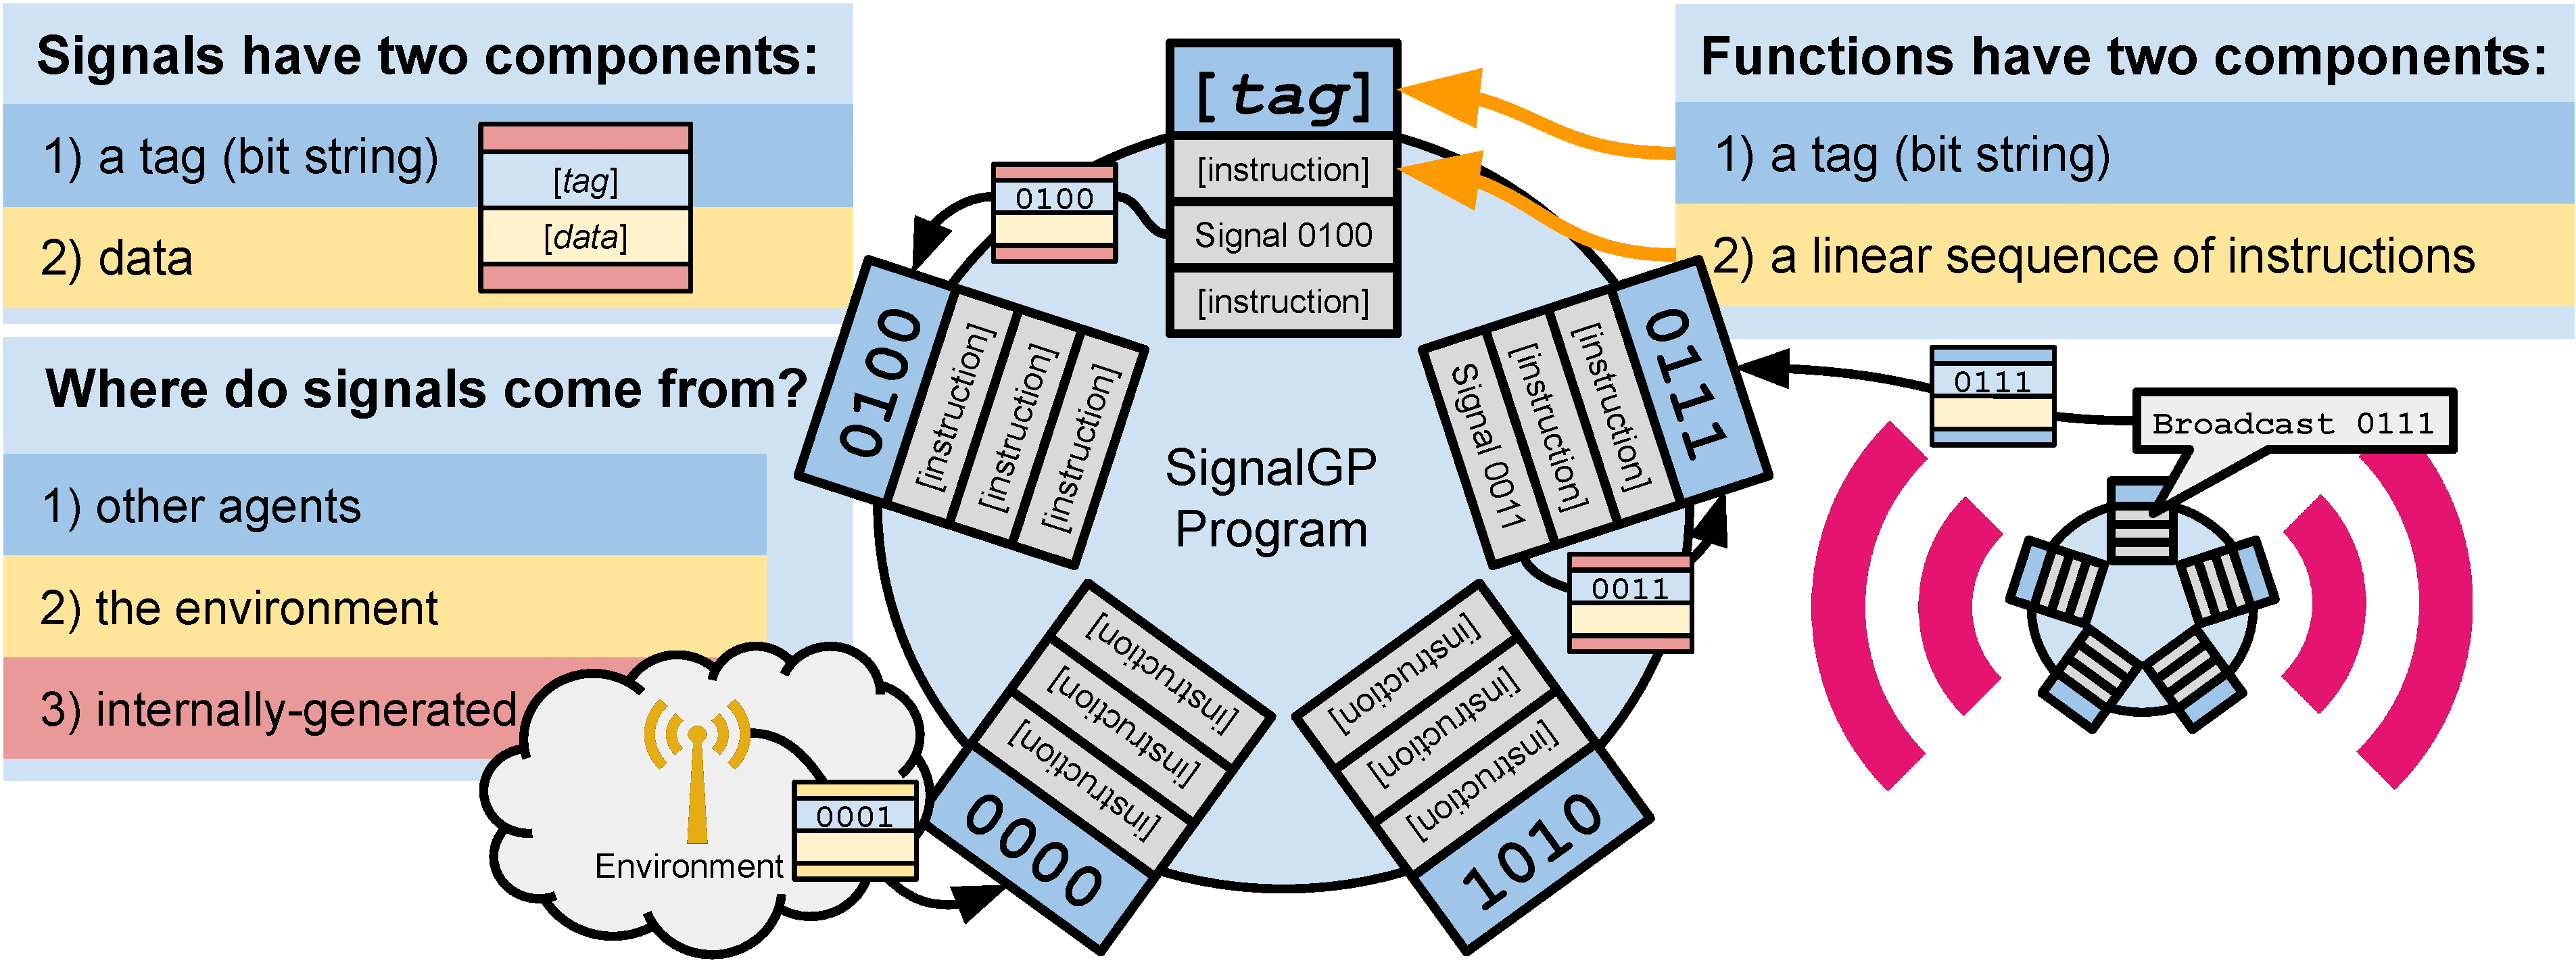
\includegraphics[width=\textwidth]
  {chapters/04-evolving-event-driven-programs-with-signalgp/media/signalgp-overview.pdf}
  \caption{\small 
  \textbf{A high-level overview of SignalGP.}
  SignalGP programs are defined by a set of functions.
  Events trigger functions with the \textit{closest matching} tag, allowing SignalGP agents to respond to signals. 
  SignalGP agents handle many events simultaneously by processing them in parallel.
  }
  \label{chapter:signalgp:fig:signalgp-overview}
\end{figure*}

\subsection{Tag-based Referencing}
\label{chapter:signalgp:sec:signalgp:tag-based-referencing}

Incorporating modules (\textit{e.g.}, functions, subroutines, macros, \textit{etc.}) into genetic programming has been extensively explored, and the benefits of modules in GP have been well documented
(\textit{e.g.}, \citep{koza_genetic_1992,koza_genetic_1994,angeline_evolutionary_1992,keijzer_undirected_2005,walker_automatic_2008,roberts_evolving_2001,spector_simultaneous_1996}). 
The main purpose of SignalGP functions are to act as event-handlers---computations triggered in response to signals. However, they have the additional benefit of providing explicit architectural support for program modularity, bestowing the boon of reusable code. 
As with any reusable code block in GP, the question remains: how should the code be referenced? 
The answer to this question can be reused to answer the following question: how should we determine which event-handlers are triggered by events? 

Inspired by John Holland's concept of a ``tag'' \citep{holland_effect_1993,holland_genetic_1987,holland_concerning_1990,holland_studying_2006} as a mechanism for matching, binding, and aggregation, Spector \textit{et al.} \citep{spector_tag-based_2011,spector_whats_2011,spector_tag-based_2012} introduced and demonstrated the value of tag-based referencing in the context of GP. 
In this context, a tag-based reference always links to a tagged entity with its closest match. 
These tagged entities include instructions and sequences of code (\textit{i.e.}, modules), providing an evolvable mechanism for code referencing. 

SignalGP shifts these ideas into a more fully event-driven context.
In SignalGP, sets of instructions are modularized into functions that are labeled with tags. Events are made explicit and trigger those functions with whose tags have the closest match.
The underlying instruction set is crafted to easily trigger internal events, broadcast external events, and to otherwise work in a tag-based context. 
Finally, SignalGP can be configured to only match tags that are relatively close (within a threshold) allowing agents to ignore events entirely by avoiding the use of similar tags.

\subsection{Virtual Hardware} 

As in many GP representations, linear GP programs are often interpreted in the context of virtual hardware, which typically comprises memory---usually in the form of registers or stacks---and other problem-specific virtual hardware elements, allowing programs to achieve complex functionality \citep{mcdermott_genetic_2015,poli_field_2008,ofria_avida:_2009}. 
SignalGP programs are interpreted by virtual hardware consisting of the following four major components: program memory, an event queue, a set of execution threads, and shared memory.

\textbf{Program memory} stores the SignalGP program currently executing on the virtual hardware.

The \textbf{event queue} manages recently received events waiting to be dispatched and processed by functions. The event queue dispatches events in the order they are received. 

The SignalGP virtual hardware supports an arbitrary number of \textbf{execution threads} that run concurrently. 
Each thread processes a single instruction every time step. 
In the same way that Byers \textit{et al.}'s parallel-executing digital enzymes \citep{byers_digital_2011} allow a robot controller to process many external stimuli simultaneously, parallel execution allows SignalGP agents to handle many events at once.

Each thread maintains a call stack that stores state information about the thread's active function calls. 
The current state for any given thread resides at the top of the thread's call stack. 
Call states maintain local state information for the function call they represent: a function pointer, an instruction pointer, input memory, working memory, and output memory. 
A function pointer indicates the current function being run. 
An instruction pointer indicates the current instruction within that function. 
Input, working, and output memory serve as local memory. 

Working memory is used for performing local operations (\textit{e.g.}, addition, subtraction, multiplication, \textit{etc.}). 
Input memory is analogous to function arguments (\textit{i.e.}, function input), and output memory is analogous to function return memory (\textit{i.e.}, what is returned when a function call concludes). 
By convention, instructions can both read from and write to working memory, input memory is read-only, and output memory is write-only. 
To use an analogy, working memory, input memory, and output memory are to SignalGP functions as hidden nodes, input nodes, and output nodes are to conventional artificial neural networks.  
\textbf{Shared memory} serves as global memory. 
Shared memory is accessible (\textit{i.e.}, readable and writable) by all threads, allowing them to store and share information. 

\subsection{Program Evaluation}

SignalGP programs are sets of functions where each function associates an evolvable tag with a linear sequence of instructions. 
In our implementation of SignalGP, instructions are argument-based, and in addition to evolvable arguments, each instruction has an evolvable tag. 
Arguments modify the effect of the instruction, often specifying memory locations or fixed values. 
Instruction tags may also modify the effect of an instruction. For example, instructions that refer to functions do so using tag-based referencing. 
Further, instructions use their tag when generating events, either to be broadcast to other SignalGP agents or to be handled internally for their own use. 

Program evaluation can be initialized either actively or passively.  
During active initialization, the program will begin evaluation by automatically calling a designated main function on a new thread.  
In passive initialization, computation takes place only in response to external events.  
In the work presented here, we use only active initialization and automatically reset the main thread if it would have otherwise terminated.

While executing, the SignalGP virtual hardware advances on each time step in three phases: 
(1) All events in the event queue are dispatched, with each triggering a function \textit{via} tag-based referencing. 
(2) Each thread processes a single instruction. 
(3) Any threads done processing are removed.
Phases occur serially and in order. 

Executed instructions may call functions, manipulate local and shared memory, generate events, perform basic computations, control execution flow, \textit{et cetera} (see supplementary material \citep{signalgp_supplement_2018} for details on all instructions used in this work).
Instructions in SignalGP are guaranteed to always be syntactically valid, but may be functionally useless. 
Every instruction has three associated arguments and an associated tag. 
Not all instructions make use of their three arguments or their tag; unused arguments and tags are not under direct selection and may drift until a mutation to the operand reveals them.

% \vspace{2mm}
% \noindent\textbf{Instruction-triggered Function Calls}\\
\subsubsection{Instruction-triggered Function Calls}

Functions in SignalGP may be triggered by either instruction calls or events.
When a \code{Call} is executed, the function in program memory with the most similar tag to the \code{Call} instruction's tag (above a similarity threshold) is triggered; in this work, ties are broken by a random draw (though any tie-breaking procedure could be used).  
Tag similarity is calculated as the proportion of matching bits between two bit strings (simple matching coefficient).  

When a function is triggered by a \code{Call} instruction, a new call state is created and pushed onto that thread's call stack.
The working memory of the caller state is copied as the input memory of the new call state (\textit{i.e.}, the arguments to the called function are the full contents of the previous working memory). 
The working memory and the output memory of the new call state are initially empty. 
To prevent unbounded recursion, we place limits on call stack depth; if a function call would cause the call stack to exceed its depth limit, the call instead behaves like a no-operation. 

Instruction-triggered functions may return by either executing a \code{Return} instruction or by reaching the end of the function's instruction sequence. 
When an instruction-triggered function returns, its call state is popped from its call stack, and anything stored in the output memory of the returning call state is copied to the working memory of the caller state (otherwise leaving the caller state's working memory unchanged). 
In this way, instruction-triggered function calls can be thought of as operations over the caller's working memory. 

% \vspace{2mm}
% \noindent\textbf{Event-triggered Function Calls}\\
\subsubsection{Event-triggered Function Calls}

Events in SignalGP are analogous to external function calls. 
When an event is dispatched from the event queue, the virtual hardware chooses the function with the highest tag similarity score (above a similarity threshold) to handle the event.
In this work, ties are broken by a random draw (though any tie-breaking procedure could be used). 

Once a function is selected to handle an event, it is called on a newly-created execution thread, initializing the thread's call stack with a new call state. 
The input memory of the new call state is populated with the event's data. 
In this way, events can pass information to the function that handles them. 
When the function has been processed (\textit{i.e.}, all of the active calls on the thread's call stack have returned), the thread is removed. 
To prevent unbounded parallelism, we place a limit on the allowed number of concurrently executing threads; if the creation of a new thread would cause the number of threads to exceed this limit, thread creation is prevented.

\subsection{Evolution}
\label{chapter:signalgp:sec:signalgp:evolution}

Evolution in SignalGP proceeds similarly to that of typical linear GP systems. 
Because function referencing is done \textit{via} tags, changes can be made to program architecture (\textit{e.g.}, inserting new or removing existing functions) while still guaranteeing syntactic correctness. 
Thus, modular program architectures can evolve dynamically through whole-function duplication and deletion operators or through function-level crossover techniques. 

In the studies presented in this paper, we evolve SignalGP programs directly (as opposed to using indirect program encodings), which requires SignalGP-aware mutation operators. 
We propagated SignalGP programs asexually and applied mutations to offspring. 
We used whole-function duplication and deletion operators (applied at a per-function rate of 0.05) to allow evolution to tune the number or functions in programs. 
We mutated tags for instructions and functions at a per-bit mutation rate (0.05). 
We applied instruction and argument substitutions at a per-instruction rate (0.005). 
Instruction sequences could be inserted or deleted via slip-mutation operators \citep{lalejini_gene_2017}, which facilitate the duplication or deletion of sequences of instructions; we applied slip-mutations at a per-function rate (0.05). 
\section{Test Problems}
\label{chapter:signalgp:sec:test-problems}

We demonstrate the value of incorporating the event-driven programming paradigm in GP using two distinct test problems: a changing environment problem and a distributed leader-election problem. 
For both problems, we compared SignalGP performance to variants that are otherwise identical, except for how they handle sensor information. 
For example, our primary variant GP must actively monitor sensors to process external signals (using the imperative paradigm).
For both test problems, a program's capacity to react efficiently to external events is crucial; thus, we hypothesized that SignalGP should perform better than our imperative alternatives.  

\subsection{Changing Environment Problem}

This first problem requires agents to coordinate their behavior with a randomly changing environment. 
The environment can be in one of $K$ possible states; to maximize fitness, agents must match their internal state to the current state of their environment. 
The environment is initialized to a random state and has a 12.5\% chance of changing to a random state at every subsequent time step.
Successful agents must adjust their internal state whenever an environmental change occurs. 

We evolved agents to solve this problem at $K$ equal to 2, 4, 8, and 16 environmental states. 
The problem scales in difficulty as the number of possible states that must be monitored increases. 
Agents adjust their internal state by executing one of $K$ state-altering instructions.
For each possible environmental state, there is an associated \code{SetState} instruction
(\textit{i.e.}, for $K=4$, there are four instructions: \code{SetState,0}, \code{SetState1}, \code{SetState2}, and \code{SetState3}).
Being required to execute a distinct instruction for each environment represents performing a behavior unique to that environment. 

We compared the performance of programs with three different mechanisms to sense the environment: 
(1) an event-driven treatment where environmental changes produce signals that have environment-specific tags and can trigger functions; 
(2) an imperative control treatment where programs needed to actively poll the environment to determine its current state; 
and (3) a combined treatment where agents are capable of using either option.  
Note that in the imperative and combined treatments we added new instructions to test each environmental state (\textit{i.e.}, for $K=4$, there are four instructions: \code{SenseEnvState0}, \code{SenseEnvState1}, \code{SenseEnvState2}, and \code{SenseEnvState3}). 
In preliminary experiments we had provided agents with a single instruction that returned the current environmental state, but this mechanism proved more challenging for them to use effectively when there were too many states (the environment ID returned by the single instruction needed to be thresholded into a true/false value, whereas the individual environment state tests directly returned a true/false value). 

% Some common loose ends across all conditions. 
Across all treatments, we added a \code{Fork} instruction to the available instruction set. 
The \code{Fork} instruction generates an internally-handled signal when executed, which provides an independent mechanism to spawn parallel-executing threads. 
The \code{Fork} instruction ensures that programs in all treatments had trivial access to parallelism. 
Because the \code{SenseEnvState} instructions in both the imperative and combined treatments bloated the instruction set relative to the event-driven treatment, we also added an equivalent number of no-operation instructions in the event-driven treatment.

% Predictions. 
\subsubsection{Hypotheses}

For low values of $K$, we expected evolved programs from all treatments to perform similarly. 
However, as continuously polling the environment is cumbersome at higher values of $K$, we expected fully event-driven SignalGP programs to drastically outperform programs evolved in the imperative treatment; further, we expected successful programs in the combined treatment to favor the event-driven strategy. 

\subsubsection{Experimental Parameters}

We ran 100 replicates of each condition at $K$ = 2, 4, 8, and 16. 
In all replicates and across all treatments, we evolved populations of 1000 agents for 10,000 generations, starting from a simple ancestor program consisting of a single function with eight no-operation instructions. 
Each generation, we evaluated all agents in the population individually three times (three trials) where each trial comprised 256 time steps. 
For a single trial, an agent's fitness was equal to the number of time steps in which its internal state matched the environment state during evaluation. 
After three trials, an agent's fitness was equal to the minimum fitness value obtained across its three trials. 
We used a combination of elite and tournament (size four) selection to select which individuals reproduced asexually each generation. 
We applied mutations to offspring as described in Section \ref{chapter:signalgp:sec:signalgp:evolution}. 
Agents were limited to a maximum of 32 parallel executing threads and a maximum of 32 functions. 
Functions were limited to a maximum length of 128 instructions. 
Agents were limited to 128 call states per call stack. 
The minimum tag reference threshold was 50\% (\textit{i.e.}, tags must have at least 50\% similarity to successfully reference). 
All tags were represented as length 16 bit strings. 

\subsubsection{Statistical Methods}

For every run, we extracted the program with the highest fitness after 10,000 generations of evolution. 
Because the sequence of environmental states experienced by an agent during evaluation are highly variant, we tested each extracted program in 100 trials, using a program's average performance as its fitness in our analyses. 
For each environment size, we compared the performances of evolved programs across treatments. 
To determine if any of the treatments were significant ($p < 0.05$) within a set, we performed a Kruskal-Wallis test. 
For an environment size in which the Kruskal-Wallis test was significant, we performed a post-hoc Dunn's test, applying a Bonferroni correction for multiple comparisons. All statistical analyses were conducted in R 3.3.2 \citep{r_core_team_2016}, and each Dunn's test was conducted using the FSA package \citep{r_FSA_2017}.

\subsection{Distributed Leader Election Problem}

In the distributed leader election problem, a network of agents must unanimously designate a single agent as leader. Agents are each given a unique identifier (UID). 
Initially, agents are only aware of their own UID and must communicate to resolve the UIDs of other agents. 
During an election, each agent may vote, and an election is successful if all votes converge to a single, consensus UID. 
This problem has been used to study the evolution of cooperation in digital systems \citep{knoester_using_2007,knoester_genetic_2013} and as a benchmark problem to compare the performance of different GP representations in evolving distributed algorithms \citep{weise_evolving_2012}. 
A common strategy for successfully electing a leader begins with all agents voting for themselves. 
Then, agents continuously broadcast their vote, changing it only when they receive a message containing a UID greater than their current vote. 
This process results in the largest UID propagating through the distributed system as the consensus leader. 
Alternatively, a similar strategy works for electing the agent with the smallest UID. 

We evolved populations of homogeneous distributed systems of SignalGP agents where networks were configured as 5x5 toroidal grids, and agents could only interact with their four neighbors. 
When evaluating a network, we initialized each agent in the network with a random UID (a number between 1 and 1,000,000). 
We evaluated distributed systems for 256 time steps. 
During an evaluation, agents retrieve their UID by executing a \code{GetUID} instruction. 
Agents vote with a \code{SetOpinion} instruction, which sets their opinion (vote) to a value stored in memory, and agents may retrieve their current vote by executing a \code{GetOpinion} instruction. 
Agents communicate by exchanging messages, either by sending a message to a single neighbor or by broadcasting a message to all neighboring agents. 

After an evaluation, we assigned fitness, $F$ according to Equation \ref{chapter:signalgp:equ:consensus-fitness} where 
$V$ gives the number of valid votes at the end of evaluation, 
$C_{\text{max}}$ gives the maximum consensus size at the end of evaluation,  
$T_{\text{consensus}}$ gives the total number of time steps at full consensus, and
$S$ gives the size of the distributed system. 


\begin{equation}
    F = V + C_{\text{max}} + (T_{\text{consensus}} \times S)
    \label{chapter:signalgp:equ:consensus-fitness}
\end{equation}

Distributed systems maximize their fitness by achieving consensus as quickly as possible and maintaining consensus for the duration of their evaluation. 
Our fitness function rewards partial solutions by taking into account valid votes (\textit{i.e.}, votes that correspond to a UID present in the network) and partial consensus at the end of an evaluation. 

We evolved distributed systems in three treatments: one with event-driven messaging and two different imperative messaging treatments. 
In the event-driven treatment, messages were events that, when received, could trigger a function. 
In both imperative treatments, messages did not automatically trigger functions; instead, messages were sent to an inbox and needed to be retrieved \textit{via} a \code{RetrieveMessage} instruction. 
The difference between the two imperative treatments was in how messages were handled once retrieved. 
In the fork-on-retrieve imperative treatment, messages act like an internally-generated event when retrieved from an inbox, triggering the function with the closest (above a threshold) matching tag on a new thread. 
In the copy-on-retrieve imperative treatment, messages are not treated as internal events when retrieved; instead, message contents are loaded into the input memory of the thread that retrieved the message. 
In the copy-on-retrieve imperative treatment, we augmented the available instruction set with the \code{Fork} instruction, allowing programs to trivially spawn parallel-executing threads. 

\subsubsection{Hypothesis}

Event-driven SignalGP agents do not need to continuously poll a message inbox to receive messages from neighboring agents, allowing event-driven programs to more efficiently coordinate. 
Thus, we expected distributed systems evolved in the event-driven treatment to outperform those evolved in the two imperative treatments. 

\subsubsection{Experimental Parameters}
We ran 100 replicates of each treatment. 
In all replicates of all treatments, we evolved populations of 400 homogeneous distributed systems for 50,000 generations. 
We initialized populations with a simple ancestor program consisting of a single function with eight no-operation instructions. 
Selection and reproduction were identical to that of the changing environment problem. 
Agents were limited to a maximum of 8 parallel executing threads. 
Agents were limited to a maximum of 4 functions, and function length was limited to a maximum 32 instructions. 
Agents were limited to 128 call states per call stack. 
The minimum tag reference threshold was 50\%. All tags were represented as length 16 bit strings. 
The maximum inbox capacity was 8. 
If a message was received and the inbox was full, the oldest message in the inbox was deleted to make room for the new message. 

\subsubsection{Statistical Methods}

For every replicate across all treatments, we extracted the program that produces the most fit distributed system after 50,000 generations of evolution. 
As in the changing environment problem, we compared treatments using a Kruskal-Wallis test, and if significant ($p < 0.05$), we performed a post-hoc Dunn's test, applying a Bonferroni correction for multiple comparisons.  

\section{Results and Discussion}
\label{chapter:signalgp:sec:results-and-discussion}

\subsection{Changing Environment Problem}


\begin{figure*}[!ht]
  \centering 
  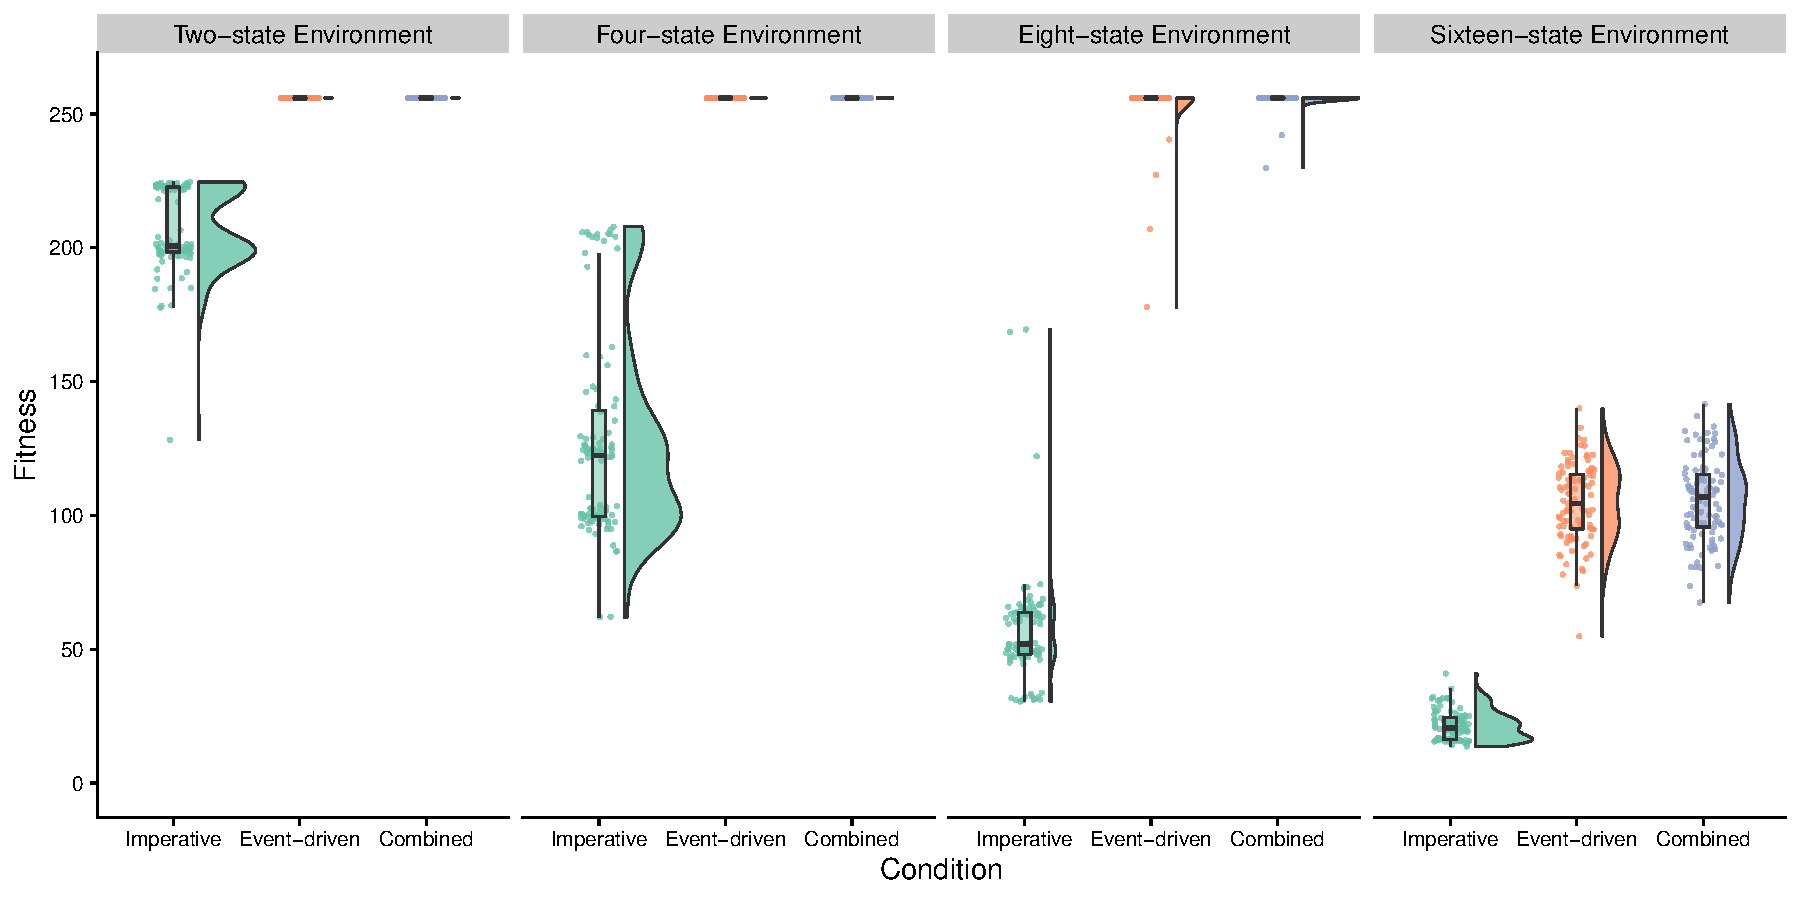
\includegraphics[width=\textwidth]{chapters/04-evolving-event-driven-programs-with-signalgp/media/chg-env-fitness.pdf}
  \caption{\small 
  Changing environment problem results across all environments: two-state environment, four-state environment, eight-state environment, and sixteen-state environment. 
  The raincloud plots \citep{allen_raincloud_2019} indicate the fitnesses (each an average over 100 trials) of best performing programs from each replicate.
  }
  \label{chapter:signalgp:fig:chg-env-fitness}
\end{figure*}


\subsubsection{Event-driven strategies outperform imperative strategies}

Figure \ref{chapter:signalgp:fig:chg-env-fitness} shows results for all environment sizes ($K$ = 2, 4, 8, and 16). 
Programs evolved in treatments with fully event-driven SignalGP significantly outperformed those evolved in the imperative treatment across all environments: two-state (combined: $p<2$e-47; event-driven: $p<2$e-47), four-state (combined: $p<2$e-47; event-driven: $p<2$e-47), eight-state (combined: $p<2$e-46; event-driven: $p<3$e-45), and sixteen-state (combined: $p<2$e-34; event-driven: $p<3$e-33). Across all environments, there was no significant difference in final program performance between the event-driven and combined treatment. 
See supplementary material for full details on statistical test results \citep{signalgp_supplement_2018}. 

Further, only treatments with fully event-driven SignalGP produced programs capable of achieving a perfect fitness of 256. 
This result is not surprising: \textit{only} programs that employ an entirely event-driven strategy can achieve a perfect score in multi-state environments. 
This is because imperative strategies must continuously poll the environment for changes, which decreases the efficiency of their response to an environmental change.
This strategy becomes increasingly cumbersome and inefficient as the complexity of the environment increases. 
In contrast, event-driven responses are triggered automatically \textit{via} the SignalGP virtual hardware, facilitating immediate reactions to environmental changes.
This allows event-driven strategies to more effectively scale with environment size than imperative strategies. 

\subsubsection{Evolution favors event-driven strategies}

In the combined treatment, evolution had access to both the event-driven (signal-based) strategy and the imperative (sensor-polling) strategy. 
As shown in Figure \ref{chapter:signalgp:fig:chg-env-fitness}, performance in the combined treatment did not significantly differ from the event-driven treatment, but significantly exceeded performance in the imperative treatment. 
However, this result alone does not reveal what strategies were favored in the combined treatment. 

%What strategy did evolution favor in the combined treatment? 
To tease this apart, we re-evaluated programs evolved under the combined treatment in two distinct conditions:
one in which we deactivated sensors and one in which we deactivated external events. 
In the deactivated sensors condition, \code{SenseEnvState} instructions behaved as no-operations, which eliminated the viability of a sensor-based polling strategy.
Likewise, the deactivated events re-evaluation condition eliminated the viability of event-driven strategies.  
Any loss of functionality by programs in these new environments will tease apart the strategies that those programs must have employed.

\begin{figure}[h]
  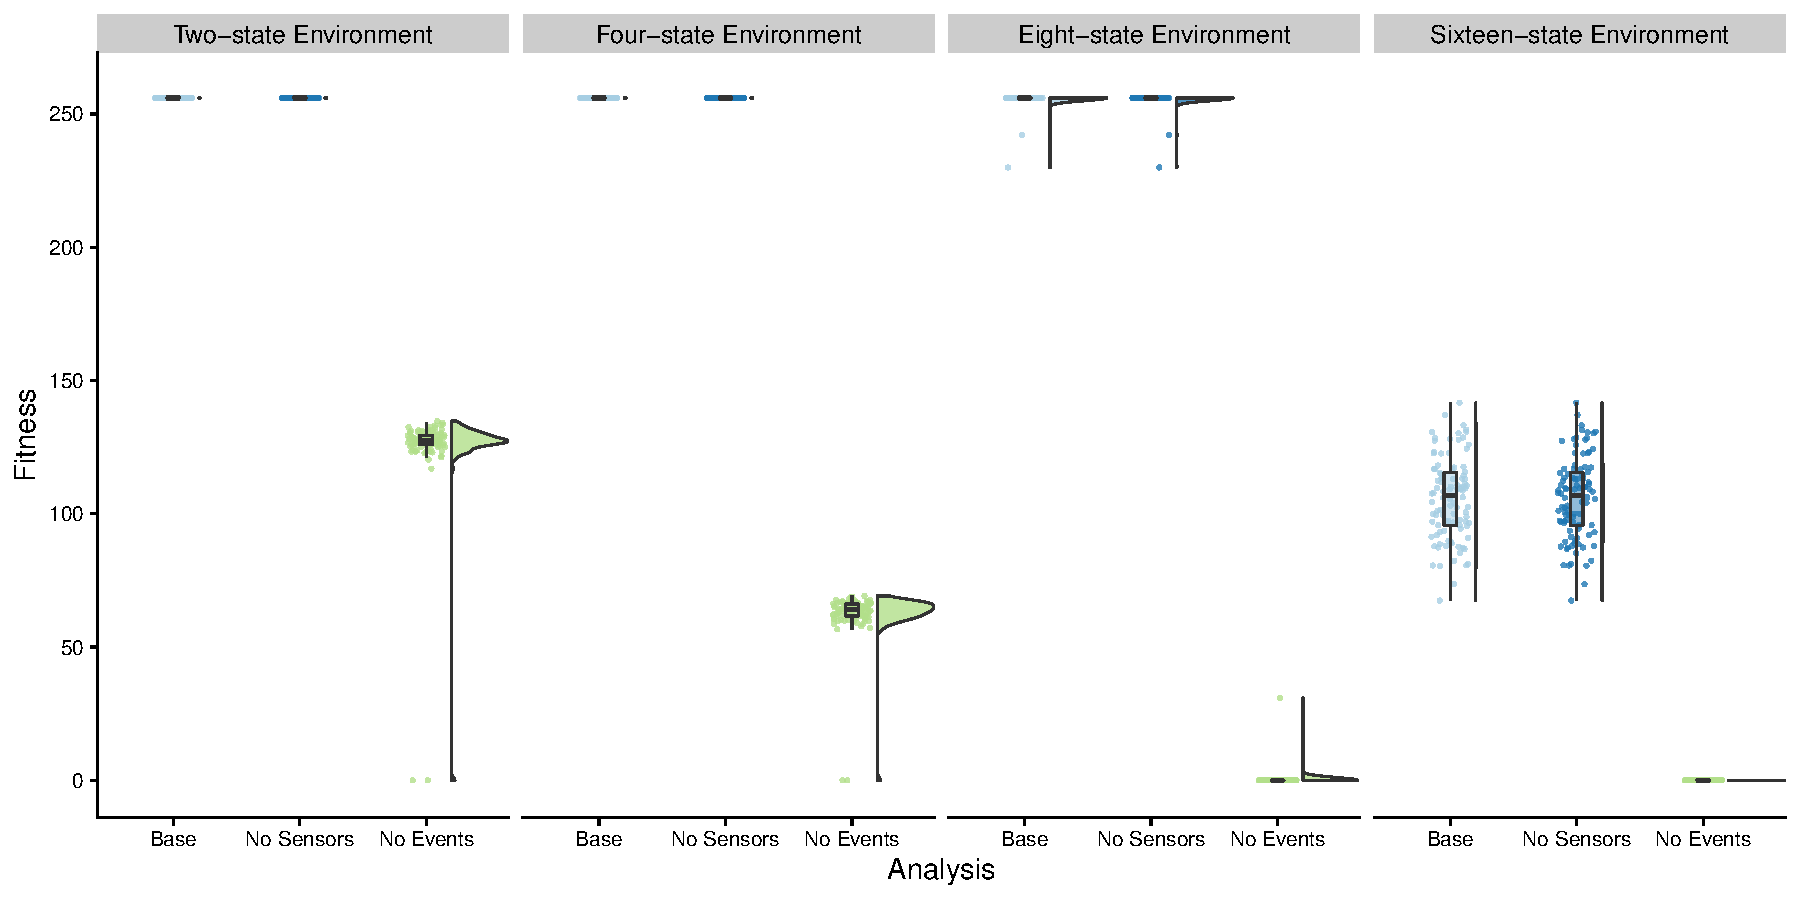
\includegraphics[width=\columnwidth]
  {chapters/04-evolving-event-driven-programs-with-signalgp/media/chg-env-combined-strategy.pdf}
  \caption{\small 
  Re-evaluation results for combined condition in the changing environment problem across all environments:  two-state environment, four-state environment, eight-state environment, and sixteen-state environment. 
  The raincloud plots indicate the fitnesses (each an average over 100 trials) of best performing programs from each re-evaluation.
  }
  \label{chapter:signalgp:fig:combined-reeval}
\end{figure}

Figure \ref{chapter:signalgp:fig:combined-reeval} shows the results of our re-evaluations. 
Across all environment sizes, there was no significant difference between program performance in their original combined condition and the deactivated sensors conditions. 
In contrast, program performances were significantly worse in the deactivated events condition than in the combined condition (two-state: $p<2$e-47; four-state: $p<2$e-47; eight-state: $p<7$e-49 ; sixteen-state: $p<4$e-35). 
These data indicate that programs evolved in the combined condition primarily rely on event-driven strategies for the changing environment problem. 

\subsection{Distributed Leader Election Problem}

\begin{figure}[h]
  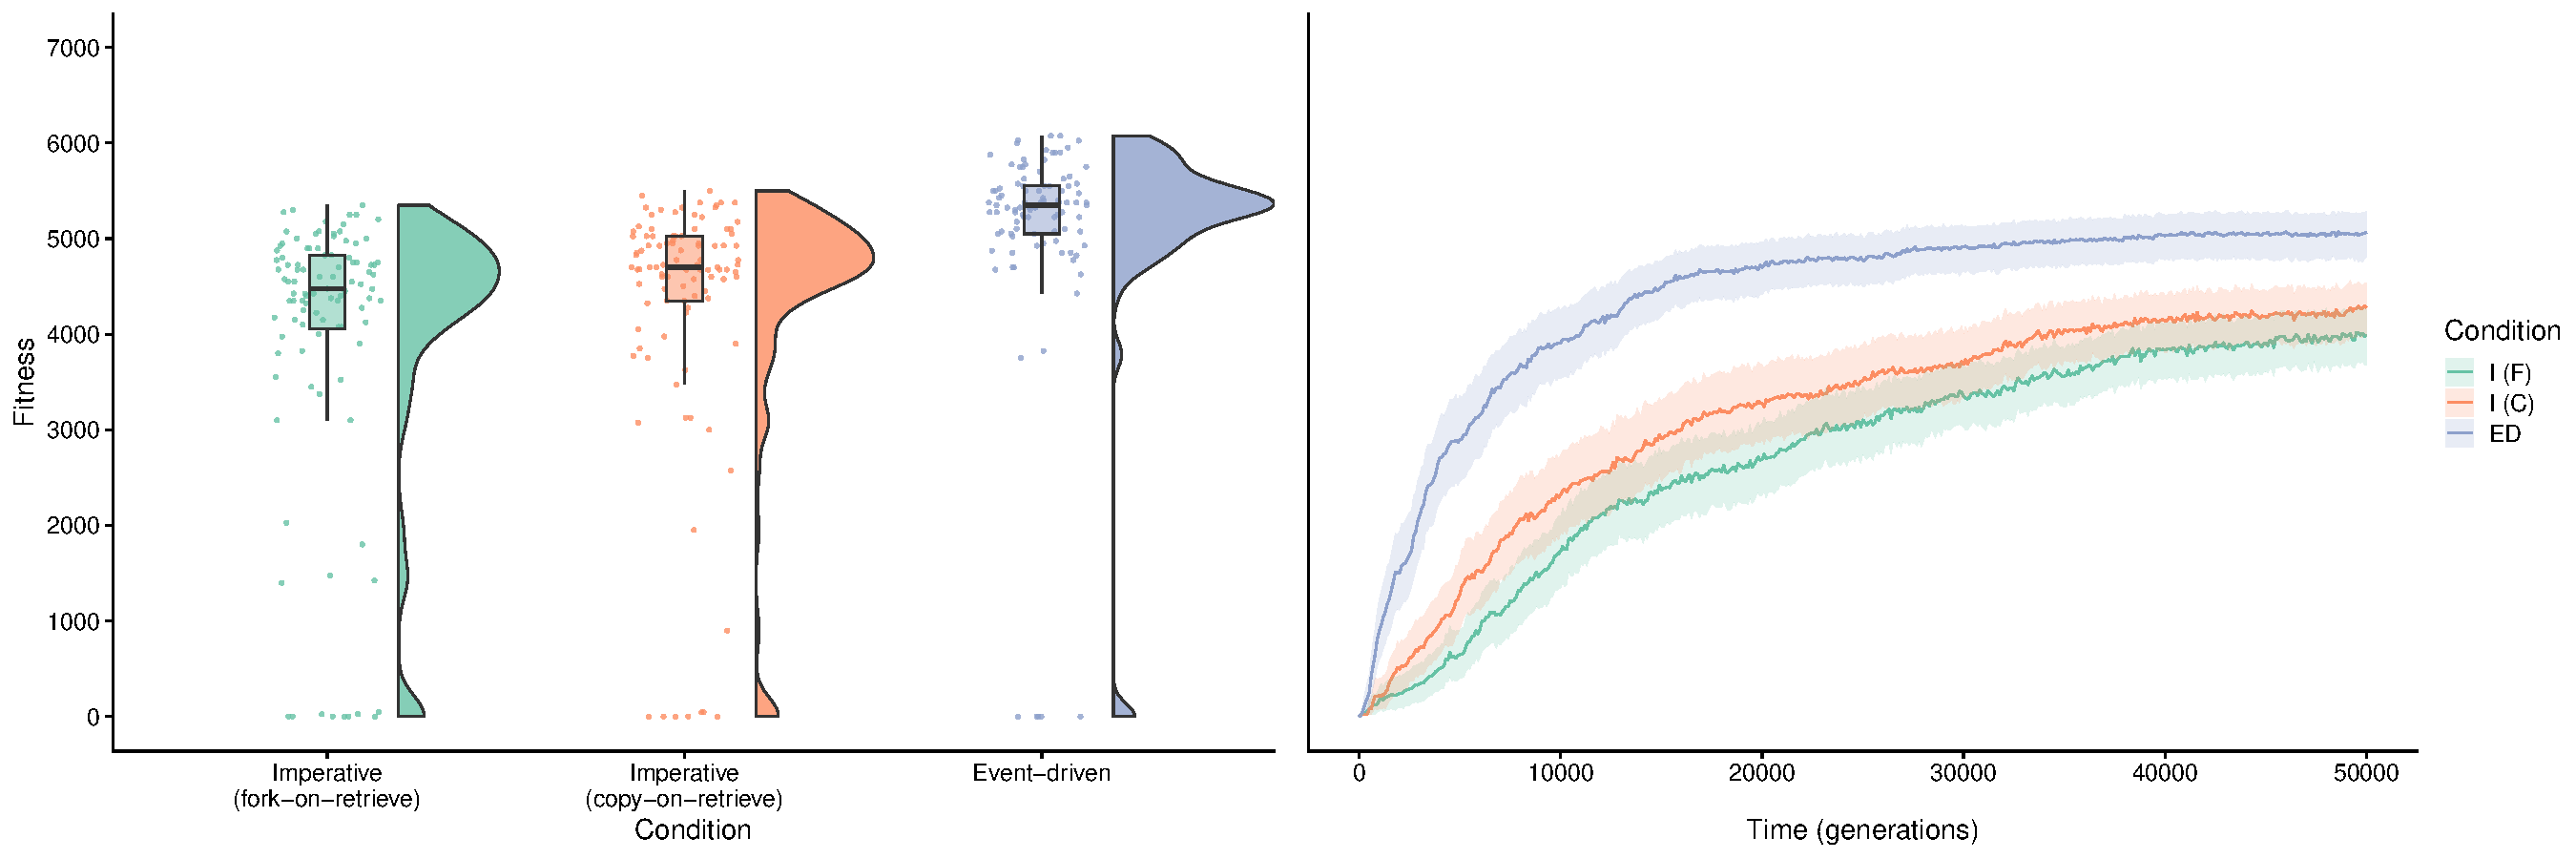
\includegraphics[width=\columnwidth]{chapters/04-evolving-event-driven-programs-with-signalgp/media/election-fitness.pdf}
  \caption{\small 
  Distributed leader election problem results. 
  The raincloud plots indicate the fitnesses of best performing distributed systems from each replicate. 
  The time series gives average fitness over time during evolution. 
  The colors in the time series correspond to the colors in the raincloud plots. 
  The shading on fitness trajectories in the time series indicates a bootstrapped 95\% confidence interval.
  }
  \label{chapter:signalgp:fig:election-fitness}
\end{figure}

% \vspace{2mm}
% \noindent\textbf{Event-driven networks outperform imperative networks.}\\
\subsubsection{Event-driven networks outperform imperative networks}

Figure \ref{chapter:signalgp:fig:election-fitness} shows the results for the distributed leader election problem.
Distributed systems evolved in the event-driven treatment significantly outperformed those evolved in both imperative treatments (fork-on-retrieval: $p<2$e-21; copy-on-retrieval: $p<2$e-13). 
See supplementary material for full details on statistical test results \citep{signalgp_supplement_2018}. 

All three conditions produced distributed systems capable of achieving election consensus. 
The difference in performances across treatments primarily reflect how quickly consensus is able to be reached within a distributed system. 
The event-driven programming paradigm is able to more efficiently encode communication between agents, as it does not require programs to continuously poll for new messages from other agents. 
Thus, the event-driven paradigm allows signals to propagate more quickly through a distributed system than the imperative paradigm. 
The time series shown in Figure \ref{chapter:signalgp:fig:election-fitness} hints that the event-driven SignalGP representation evolves more rapidly for the distributed leader election problem than the imperative variants; however, deeper analyses are required for confirmation. 


\section{Conclusion}

We introduced SignalGP, a new type of GP technique designed to provide evolution direct access to the event-driven programming paradigm by augmenting Spector \textit{et al.}'s \citep{spector_tag-based_2011} tag-based modular program framework. 
We have described and demonstrated SignalGP within the context of linear GP. 
Additionally, we used SignalGP to explore the value of capturing the event-driven paradigm on two problems where the capacity to react to external signals is critical: the changing environment problem, and the distributed leader election problem. 
At a minimum, our results show that access to the event-driven programming paradigm allows programs to more efficiently encode agent-agent and agent-environment interactions, resulting in higher performance on both the changing environment and distributed leader election problems. 
Deeper analyses are needed to tease apart the effects of the event-driven programming paradigm on the evolvability of solutions. 

\subsection{Beyond Linear GP}

While this work presents SignalGP in the context of linear GP, the ideas underpinning SignalGP are generalizable across a variety of evolutionary computation systems. 

We can imagine SignalGP functions to be black-box input-output machines. 
Here, we have exclusively put linear sequences of instructions inside these black-boxes, but could have easily put other representations capable of processing inputs (\textit{e.g.}, other forms of GP, Markov brains \citep{hintze_markov_2017}, artificial neural networks, \textit{etc.}).
We could even employ black-boxes with a variety of different contents within the same agent. 
Encasing a variety of representations within a single agent may complicate the virtual hardware, program evaluation, and mutation operators, but also provides evolution with a toolbox of diverse representations.

As we continue to explore the capabilities of SignalGP, we plan to explore the evolvability of event-driven programs versus imperative programs across a wider set of problems and incorporate comparisons to other GP representations. 
Further, we plan to extend SignalGP to other representations beyond linear GP and compare their relative capabilities and interactions.

\section{Software and Data Availability}

We implemented SignalGP, the changing environment problem, and the distributed leader election problem using the Empirical scientific software library \citep{charles_ofria_2020_empirical}. 
We conducted all statistical analyses for this work using R version 3.3.2 \citep{r_core_team_2016}.
Our source code for test problems, experiment data, and analyses can be found in supplemental material \citep{signalgp_supplement_2018}, which is hosted on GitHub\footnote{https://github.com/amlalejini/GECCO-2018-Evolving-Event-driven-Programs-with-SignalGP/}. 


\chapter{Improving context-dependent problem solving with a tag-based approach to regulating genetic programming modules}
\label{chapter:tag-based-regulation}

%%%%%%%%%%%%%%%%%%%%%%%%%%%%%%%%%%%%%%%%%%%%%%%%%%%%%%%%%%%
% Utility variables used in paper
%%%%%%%%%%%%%%%%%%%%%%%%%%%%%%%%%%%%%%%%%%%%%%%%%%%%%%%%%%%

%%%%%%%%%%%%%%%%%%%%%%%%%%%%%%%%%%%%
% Utility commands
%%%%%%%%%%%%%%%%%%%%%%%%%%%%%%%%%%%%
\newcolumntype{Y}{>{\centering\arraybackslash}X}

%%%%%%%%%%%%%%%%%%%%%%%%%%%%%%%%%%%%
% supplemental material
%%%%%%%%%%%%%%%%%%%%%%%%%%%%%%%%%%%%

\newcommand{\supSecDataAvailability}{Section 2}
\newcommand{\supSecStreakMetric}{Section 5}
\newcommand{\supSecRepeatedSigAnalysis}{Section 7}
\newcommand{\supSecContextSigAnalysis}{Section 8}
\newcommand{\supSecBooleanCalcPrefixAnalysis}{Section 9}
\newcommand{\supSecChangingSigAnalysis}{Section 10}
\newcommand{\supSecBooleanCalcPostfixAnalysis}{Section 11}
\newcommand{\supSecHandcodedPrograms}{Section 12}

%%%%%%%%%%%%%%%%%%%%%%%%%%%%%%%%%%%%
% Evolution parameters
%%%%%%%%%%%%%%%%%%%%%%%%%%%%%%%%%%%%
\newcommand{\MutRateInstArgSub}{0.001}

\newcommand{\MutRateInstSub}{0.001}
\newcommand{\MutRateInstIns}{0.001}
\newcommand{\MutRateInstDel}{0.001}
\newcommand{\MutRateInstPoint}{0.001}

\newcommand{\MutRateSeqSlip}{0.05}

\newcommand{\MutRateFuncDup}{0.05}
\newcommand{\MutRateFuncDel}{0.05}

\newcommand{\MutRateInstTagBF}{0.0001}
\newcommand{\MutRateFuncTagBF}{0.0001}
\newcommand{\MutRateTagBF}{0.0001}

\newcommand{\MaxFuncCnt}{256}
\newcommand{\MaxFuncInstCnt}{128}

\newcommand{\MinArgValue}{\nobreakdash-4}
\newcommand{\MaxArgValue}{4}

%%%%%%%%%%%%%%%%%%%%%%%%%%%%%%%%%%%%
% Repeated-signal task parameters
%%%%%%%%%%%%%%%%%%%%%%%%%%%%%%%%%%%%
\newcommand{\RepeatSigTaskCpuTimePerSignal}{128}

%%%%%%%%%%%%%%%%%%%%%%%%%%%%%%%%%%%%
% Contextual-signal task parameters
%%%%%%%%%%%%%%%%%%%%%%%%%%%%%%%%%%%%
\newcommand{\ContextSigTaskCpuTimePerSignal}{128}

%%%%%%%%%%%%%%%%%%%%%%%%%%%%%%%%%%%%
% Boolean logic calculator task parameters
%%%%%%%%%%%%%%%%%%%%%%%%%%%%%%%%%%%%
\newcommand{\CalculatorTaskCpuTimePerSignal}{128}

%%%%%%%%%%%%%%%%%%%%%%%%%%%%%%%%%%%%
% Repeated-signal task results
%%%%%%%%%%%%%%%%%%%%%%%%%%%%%%%%%%%%
% FROM - 2020-11-25-rep-sig
%%% TWO SIGNAL %%%
\newcommand{\RSPTwoSigRegOnlySolutionCnt}{200}
\newcommand{\RSPTwoSigMemOnlySolutionCnt}{137}
\newcommand{\RSPTwoSigBothSolutionCnt}{200}
%%% FOUR SIGNAL %%%
\newcommand{\RSPFourSigRegOnlySolutionCnt}{200}
\newcommand{\RSPFourSigMemOnlySolutionCnt}{8}
\newcommand{\RSPFourSigBothSolutionCnt}{200}
%%% EIGHT SIGNAL %%%
\newcommand{\RSPEightSigRegOnlySolutionCnt}{198}
\newcommand{\RSPEightSigMemOnlySolutionCnt}{0}
\newcommand{\RSPEightSigBothSolutionCnt}{198}
%%% SIXTEEN SIGNAL %%%
\newcommand{\RSPSixteenSigRegOnlySolutionCnt}{73}
\newcommand{\RSPSixteenSigMemOnlySolutionCnt}{0}
\newcommand{\RSPSixteenSigBothSolutionCnt}{74}

% --- (KO) STRATEGIES (condition=regulation-augmented/memory+regulation) ---
%%% TWO SIGNAL %%%
\newcommand{\RSPTwoSigRegOnlyStrategyCnt}{188}
\newcommand{\RSPTwoSigMemOnlyStrategyCnt}{11}
\newcommand{\RSPTwoSigBothStrategyCnt}{1}

\newcommand{\RSPTwoSigRegRequiredStrategyCnt}{189}
\newcommand{\RSPTwoSigUnsolvedCnt}{0}

%%% FOUR SIGNAL %%%
\newcommand{\RSPFourSigRegOnlyStrategyCnt}{177}
\newcommand{\RSPFourSigMemOnlyStrategyCnt}{0}
\newcommand{\RSPFourSigBothStrategyCnt}{23}

\newcommand{\RSPFourSigRegRequiredStrategyCnt}{200}
\newcommand{\RSPFourSigUnsolvedCnt}{0}

%%% EIGHT SIGNAL %%%
\newcommand{\RSPEightSigRegOnlyStrategyCnt}{183}
\newcommand{\RSPEightSigMemOnlyStrategyCnt}{0}
\newcommand{\RSPEightSigBothStrategyCnt}{15}

\newcommand{\RSPEightSigRegRequiredStrategyCnt}{198}
\newcommand{\RSPEightSigUnsolvedCnt}{2}

%%% SIXTEEN SIGNAL %%%
\newcommand{\RSPSixteenSigRegOnlyStrategyCnt}{71}
\newcommand{\RSPSixteenSigMemOnlyStrategyCnt}{0}
\newcommand{\RSPSixteenSigBothStrategyCnt}{3}

\newcommand{\RSPSixteenSigRegRequiredStrategyCnt}{74}
\newcommand{\RSPSixteenSigUnsolvedCnt}{126}
%%%%%%%%%%%%%%%%%%%%%%%%%%%%%%%%%%%%
% Contextual-signal task results
%%%%%%%%%%%%%%%%%%%%%%%%%%%%%%%%%%%%
% From - 2020-11-27

\newcommand{\ContextFourSigMemOnlySolutionCnt}{173}
\newcommand{\ContextFourSigBothSolutionCnt}{200}

% --- (KO) STRATEGIES (condition=regulation-augmented/memory+regulation) ---
\newcommand{\ContextFourSigMemOnlyStrategy}{0}
\newcommand{\ContextFourSigRegOnlyStrategy}{105}
\newcommand{\ContextFourSigBothStrategy}{95}

%%%%%%%%%%%%%%%%%%%%%%%%%%%%%%%%%%%%
% Changing-signal task results
%%%%%%%%%%%%%%%%%%%%%%%%%%%%%%%%%%%%
% From - 

\newcommand{\ChangingSigSixteenSigMemOnlySolutionCnt}{X}
\newcommand{\ChangingSigSixteenSigBothSolutionCnt}{X}

%%%%%%%%%%%%%%%%%%%%%%%%%%%%%%%%%%%%
% Boolean Logic Calculator (PREFIX) results
%%%%%%%%%%%%%%%%%%%%%%%%%%%%%%%%%%%%
% From - 

\newcommand{\BoolCalcPrefixMemOnlySolutionCnt}{X}
\newcommand{\BoolCalcPrefixBothSolutionCnt}{X}

%%%%%%%%%%%%%%%%%%%%%%%%%%%%%%%%%%%%
% Boolean Logic Calculator (POSTFIX) results
%%%%%%%%%%%%%%%%%%%%%%%%%%%%%%%%%%%%
% From - 

\newcommand{\BoolCalcPostfixMemOnlySolutionCnt}{X}
\newcommand{\BoolCalcPostfixBothSolutionCnt}{X}

\noindent
Authors: Alexander Lalejini, Matthew Andres Moreno, and Charles Ofria \\
This chapter is adapted from ~\citep{lalejini2020tagbased}, which has been accepted for publication in Genetic Programming and Evolvable Machines.

\section{Introduction}

% - Introduce genetic programming and automatic program synthesis + state what we do -
Genetic programming (GP) applies the natural principles of evolution to automatically synthesize programs rather than writing them by hand.
Indeed, the promise of automating computer programming has motivated advances in GP since its early successes in the 1980s \citep{forsyth_beagle_1981,cramer_representation_1985,koza_hierarchical_1989}. 
Just as human software developers have access to a dazzling array of programming languages, each specialized for solving different types of problems, GP features many ways to represent evolvable programs.
Each representation features different programmatic elements that vary in their syntax, organization, interpretation, and evolution.
These differences can dramatically influence the types of computer programs that can be evolved, and as such, influence a representation's problem-solving range \citep{hintze_buffet_2019,wilson_comparison_2008}. 
Here, we introduce and experimentally demonstrate tag-based module regulation for genetic programming, allowing us to more easily evolve programs capable of dynamically regulating responses to inputs over time.

%%%%%%%%%%%% lit to cite
% - TO READ (for different representations = different problem-solving):
%   - A Comparison of Cartesian Genetic Programming and Linear Genetic Programming
%%%%%%%%%%%%

% - Introduce value of software 'plasticity', link plasticity and modularity - 
Nearly all software applications are capable of conditionally responding to inputs.
For example, each input button on a calculator triggers a different software response; or, in the Small or Large problem from the Helmuth and Spector's automatic program synthesis benchmark suite \citep{helmuth_general_2015}, programs must output different classifications (``small'', ``large'', or ``neither'') depending on a numeric input value.
Just like such conditional logic is inherent in any non-trivial software, so to is it ubiquitous in biological organisms where it is referred to as ``plastic'' behavior or ``phenotypic plasticity.''
%Just like these dynamic responses are inherent in any non-trivial software, so to are they ubiquitous in natural organisms where they are referred to as ``plastic'' behaviors or ``phenotypic plasticity''.

% - link modular software design to improved software 'plasticity' -
Modular software design --- that is, designs that promote the partitioning and reusability of functional units --- is fundamental to good software development practices; this principle is all the more true in producing programs capable of complex ``plasticity.'' 
% Modular software design --- that is, designs that enable the separability and reusability of functional units --- is fundamental to good software development practices; this principle is all the more true in producing programs capable of complex ``plasticity''. 
By modularizing code (\textit{e.g.}, into functions, classes, libraries, \textit{etc.}), software developers can craft customized responses to inputs by composing relevant modules.  
These modules can each contain segments of code whose functionality would otherwise need to be reinvented for each response.
Likewise, modularity appears to be critical in natural genomes \citep{wagner_road_2007} as well as artificial evolving systems \citep{huizinga_does_2016}.
Moreover, evidence in these evolving systems suggests that modularity can improve the capacity for effective plasticity to arise \citep{londe_phenotypic_2015,ellefsen_neural_2015}. % and problem solving success?

Developing GP systems that facilitate the evolution of modular program architectures has long captured the attention of the genetic programming community. 
Koza introduced Automatically Defined Functions (ADFs) where callable functions can evolve as separate branches of GP syntax trees \citep{koza_genetic_1992,koza_genetic_1994}.
Angeline and Pollack developed compression and expansion genetic operators to automatically modularize existing code into libraries of parameterized subroutines \citep{angeline_evolutionary_1992}. 
Since these foundational advances, significant efforts have been made to allow GP representations to incorporate internal modules 
(\textit{e.g.},
\citep{spector_simultaneous_1996,oneill_grammar_2000,binard_abstraction-based_2007,walker_automatic_2008,spector_tag-based_2011,spector_tag-based_2012,lalejini_evolving_2018}),
to measure (and select for) modularity in evolving programs 
(\textit{e.g.}, \citep{krawiec_functional_2009,saini_modularity_2019,saini_using_modularity_2020}),
and to build ``libraries'' of reusable code modules accessible to evolving populations of programs
(\textit{e.g.}, \citep{rosca_learning_1994,banscherus_hierarchical_2001,keijzer_run_2004,keijzer_undirected_2005}).

% - Introduce more complicated form of plasticity -
These innovations have improved the ability of GP systems to link modules together to solve problems, thus improving their prospects as general-purpose tools for automatic program synthesis.
In existing GP work, links between modules, however, are typically hard coded and static during program execution; 
less is known for how to evolve programs that can adjust module associations on the fly.
For many types of problems, the appropriate set of modules to execute in response to a particular input changes over time.
This requires programs to continuously adjust associations between inputs and modular responses based on context.
For example, the computations that occur on a calculator after pressing the ``equals'' button are \textit{context-dependent}; that is, they depend on the set of operators and operands (\textit{i.e.}, inputs) previously provided. 
To achieve this design pattern, programs must internally track contextual information and typically regulate responses using explicit flow control directives (such as if-statements).
Our goal is to evolve programs that dynamically regulate modules during execution to more effectively solve context-dependent problems.  
To reach this goal, we draw inspiration from gene regulatory networks (both natural and artificial) to augment how program modules are called in GP.

% - Introduce what we did, summarize our findings -
Here, we propose to facilitate dynamic module composition by introducing tag-based module regulation for genetic programming. 
We extend existing tag-based naming schemes to allow programs to dynamically adjust associations between references and code modules. 
We experimentally demonstrate our implementation of tag-based genetic regulation in the context of SignalGP \citep{lalejini_evolving_2018}; however, our approach is immediately applicable to any existing tag-enabled GP system, such as tag-addressed Run Transferable Libraries \citep{keijzer_run_2004} or PushGP \citep{spector_tag-based_2011}.
We add ``regulation'' instructions to SignalGP that can adjust (\textit{i.e.}, promote or repress) which code modules respond to input signals and internal calls.
This extension allows evolution to structure a program as a gene regulatory network where genes are program modules and program instructions mediate regulation.
We show that module regulation improves problem-solving performance on problems where responses to particular inputs change depending on prior context (\textit{e.g.}, prior inputs). 
We also observe that our implementation of tag-based regulation can impede adaptive evolution when outputs are not context-dependent. 
% (\textit{i.e.}, the correct response to a particular input does not change over time).


\section{Specifying Modules with Tag-based Referencing}
\label{chapter:tag-based-regulation:sec:tag-based-referencing}
% Alternatively, just 'Tag-based Referencing'

% - motivation for evolvable names -
All programming representations that support modularizing code into functions or libraries define mechanisms for labeling and subsequently referencing modules. 
In traditional software development, programmers hand label modules and reference a particular module using its assigned label.
Programmers must precisely name the module they intend to reference; imprecision typically results in incorrect outputs or a syntax error. 
This mechanism for referencing modules allows for an arbitrarily large space of possible module names and is intentionally brittle, ensuring programs are either interpreted by a computer exactly as written or not interpreted at all. 
Requiring genetic programming systems to adhere to these traditional approaches to module referencing is not ideal. 
Mutation operators must either ensure that mutated labels are syntactically valid, or else cope with an abundance of broken code.
These choices result in either a search space that is overly constrained or one that is rugged and difficult to navigate \citep{rasmussen_coreworld_1990}.

% - tag-based referencing (definition) -
Inspired by Holland's use of ``tags'' to facilitate binding and aggregation in complex adaptive systems \citep{holland_concerning_1990,holland_effect_1993}, %XXX implemented [citations] and then 
Spector \textit{et al.} generalized the use of tags to label and refer to program modules in GP \citep{spector_tag-based_2011,spector_whats_2011}.
Tags are evolvable labels that can be mutated, and the similarity (or dissimilarity) between any two tags can be quantified. 
Tags are most commonly represented as floating point or integer numeric values \citep{keijzer_run_2004,spector_tag-based_2011} or as bit strings \citep{lalejini_evolving_2018}.
Like traditional naming schemes, tags can provide an arbitrarily large address space.
Unlike traditional naming schemes, however, tags allow for \textit{inexact} addressing. 
A referring tag targets the tagged entity (\textit{e.g.}, a module) with the \textit{closest matching} tag; 
this ensures that all possible tags are valid references.
Further, mutations to tags do not necessarily invalidate existing references.
For example, mutating a referring tag will have no phenotypic effect if those mutations do not change which target tag is matched. 
As such, mutating tag-based names is not necessarily catastrophic to program functionality, allowing the labeling and use of modularized code fragments to incrementally co-evolve \citep{spector_tag-based_2011}.
%tag-based naming schemes allow the labeling and use of modularized code fragments to incrementally co-evolve \citep{spector_tag-based_2011}.

% - history/background for tag-based referencing -
Tag-based referencing has long been used to expand the capabilities of genetic programming systems.
Keijzer \textit{et al.} created Run Transferable libraries of tag-addressable functions using successful code segments evolved in previous GP runs \citep{keijzer_run_2004,keijzer_undirected_2005}.
Evolving programs (represented as program trees) contained dynamically-linked nodes that used tag-based referencing to call library functions.
These tag-addressed libraries were updated between runs and did not co-evolve with programs.

Spector \textit{et al.} augmented PushGP with tag-based referencing, allowing tag-addressable code modules to evolve \textit{within} a program \citep{spector_tag-based_2011}.
Spector \textit{et al.} found that tags provided a flexible mechanism for modularization that allowed tag-enabled programs to better scale with problem size. 
Additionally, Spector \textit{et al.} expanded tag-based modules beyond PushGP, successfully applying the technique to tree-based GP \citep{spector_tag-based_2012}.

Lalejini and Ofria further extended tag-based naming to linear GP.  
Their SignalGP system broadens the application of tags to facilitate the evolution of event-driven programs \citep{lalejini_evolving_2018,lalejini_what_2019}. 
In SignalGP, tagged modules are called internally or triggered in response to tagged events (\textit{e.g.}, events generated by other agents or the environment).
More recently, Lalejini and Ofria demonstrated the use of tags to label memory positions in GP, enabling programs to define and use evolvable variable names \citep{lalejini_tag-accessed_2019}.
This tag-based memory implementation did not substantively affect problem-solving performance; however, tag-based addressing features a larger addressable memory space than more traditional register-based memory approaches in GP.
% @AML: Anything from DISHTINY we should cite?
\section{Tag-based Genetic Regulation}
\label{chapter:tag-based-regulation:sec:tag-based-genetic-regulation}

Here, we allow programs to use tag-based referencing to dynamically regulate module execution.
To achieve this, we draw inspiration from both natural and artificial gene regulatory networks. 
We demonstrate that this approach promotes more effective solutions for context-dependent problems.

% - gene regulation background, briefly -
Gene regulatory networks represent the complex interactions among genes, transcription factors, and signals from the environment that, together, control gene expression \citep{banzhaf_artificial_2015}.
Gene regulation allows for feedback loops so that prior events can continue to influence future expression in flexible and nuanced ways. 
Gene regulation underlies most important biological processes, including cell differentiation, metabolism, the cell cycle, and signal transduction \citep{karlebach_modelling_2008}.
The role of gene regulatory networks in sustaining complex life has inspired varied and abundant computational models of these networks \citep{cussat-blanc_artificial_2019,karlebach_modelling_2008}.

Artificial gene regulatory networks have been used to study how natural gene regulation evolves \citep{aldana_robustness_2007,crombach_evolution_2008,draghi_evolutionary_2009} and as a tool in evolutionary computation to solve challenging control problems (as reviewed by \citep{cussat-blanc_artificial_2019}).
Evolved artificial gene regulatory networks have even been used as indirect encoders, providing a developmental phase to translate genomes into programs \citep{banzhaf_artificial_2003,lopes_regulatory_2012} or neural networks \citep{kowaliw_using_2014}.
La Cava \textit{et al.} demonstrated a form of \textit{epigenetic} regulation for genetic programming where ``gene'' activation and silencing is learned each generation \citep{la_cava_genetic_2015,la_cava_inheritable_2015}; however, the programs themselves did not have direct control over these regulatory elements.
Inspired by chromatin remodeling in biological cells, Turner \textit{et al.} introduced artificial epigenetic networks that allow for the regulation (\textit{i.e.}, the addition or removal) of internal network components  \citep{turner_artificial_2017}; such topological self-modification improved problem-solving success for dynamical control problems.

We aim to incorporate gene regulatory network-inspired methodology to allow programs to dynamically adjust which module is triggered by a particular call based on not just current inputs, but also prior inputs.
We achieved this goal by instantiating gene regulatory networks using tag-based referencing.
Specifically, we implemented tag-based genetic regulation in the context of the linear GP system SignalGP \citep{lalejini_evolving_2018}, which is described in further detail in Section \ref{chapter:tag-based-regulation:sec:methods:signalgp}.
Here, we describe tag-based genetic regulation in terms of our SignalGP-based implementation; however, our overall approach is immediately applicable to each of the tag-enabled systems described in Section \ref{chapter:tag-based-regulation:sec:tag-based-referencing} and can be easily incorporated into any genetic programming representation.

Briefly, programs in SignalGP are composed of tag-addressed modules (\textit{i.e.}, functions), each of which contain a linear sequence of instructions. 
Each instruction has arguments, including an evolvable tag that can be used to identify and call a tag-addressed module.
When a referring tag (\textit{e.g.}, from an instruction) is used to look up a tag-addressed module, all modules in that program are ranked according to a tag-matching score. 
A tag-matching score quantifies the quality of the reference between a referring tag and a module's tag; we always select the module with best reference quality (\textit{i.e.}, the highest tag-match score with the referring tag).
When a module is called, it is executed procedurally, instruction-by-instruction, in the same way as in a conventional linear GP system. 

\begin{figure}[ht!]
    \centering
    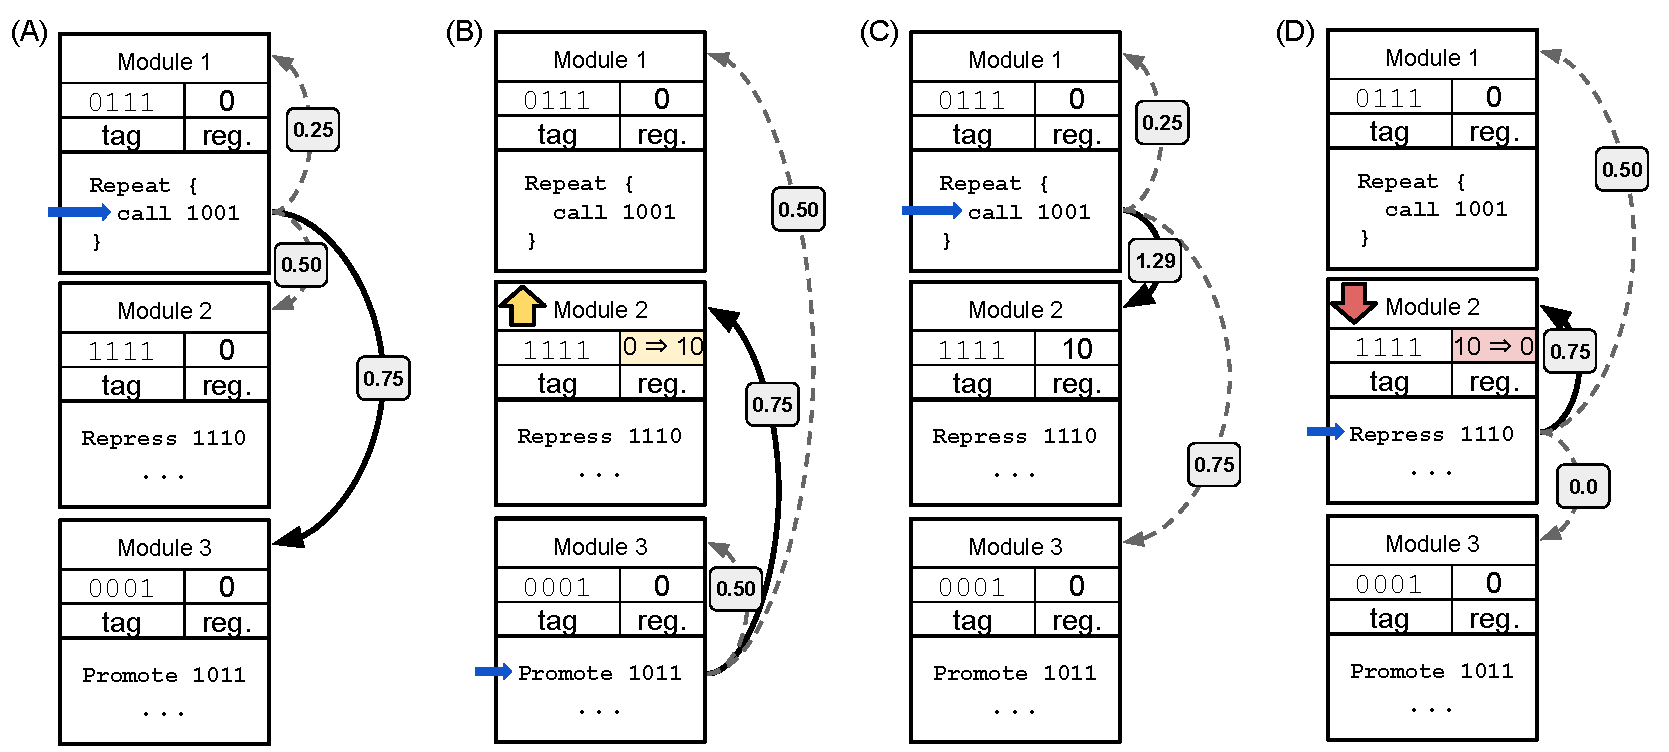
\includegraphics[width=\textwidth]{chapters/05-tag-based-genetic-regulation/media/regulation-example.pdf}
    \caption{\small
    \textbf{Tag-based genetic regulation example.}
    This example depicts a simple oscillating regulatory network instantiated using tag-based regulation.
    In this example, tags are length-4 bit strings. 
    The ``raw'' match score between two tags equals the number of matching bits between them.
    Regulation (reg.) modifies match scores for ``\code{call}'' instructions according to Equation \ref{chapter:tag-based-regulation:equ:reg-transform}.
    First (A), the \code{call 1001} in Module 1 executes, triggering Module 3. 
    Next (B), Module 3 is executed, promoting Module 2. 
    After Module 3 returns, the \code{call 1001} in Module 1 executes again (C); however, Module 2's promotion causes it to be triggered instead of Module 3. 
    Finally (D), Module 2 executes and represses itself, resetting its regulatory modifier to 0. 
    }
    \label{chapter:tag-based-regulation:fig:regulation-example}
\end{figure}


We modified SignalGP in two ways to implement tag-based genetic regulation: 

\begin{enumerate}
    \item We added a ``regulatory modifier'' value (represented as a floating point value) to all tag-addressed modules. A module's regulatory modifier adjusts how well that module matches to referring tags, and thus, modifies the likelihood it will be referenced.
    \item We supplemented the instruction set with promoter and repressor instructions that, when executed, adjust a target module's regulatory modifier. 
\end{enumerate} 

When a program begins execution, each internal module initially has no regulatory modification.\footnote{
    Alternatively, allowing programs to inherit their parent's regulatory modifiers can provide a simple model of epigenetics.
}
When a promoter or repressor instruction is executed, its associated tag identifies which module should be regulated using tag-based referencing.
Promoter instructions increase a target module's regulatory modifier, which increases the module's tag-match score with subsequent references (according to equation \ref{chapter:tag-based-regulation:equ:reg-transform} below) and thus increases the module's chances of being referenced.
Repressor instructions have the opposite effect.
Regulatory modifiers can be configured to persist over a program's entire execution or passively decay over time.

When determining which module to call at runtime, each module's tag-match score is a function of how well the module's tag matches the call instruction's tag as modified by the module's regulatory value.
If a module's regulatory modifier has been sufficiently decreased by repressor instructions, it is possible that the module will no longer be able to be referenced, as its regulated tag-match score will always be lower than at least one other program module.
We must ensure that this situation does not create an unrecoverable regulatory state and that such a fully repressed module can always be restored.
As such, promoter and repressor instructions use \textit{unregulated} tag-based referencing to identify which modules they regulate; that is, we do not apply regulatory modifiers to tag-based references made by promoter and repressor instructions. 
This ensures that no matter how much a particular module has been repressed, subsequent promoter instructions can increase its regulatory modifier.
Figure \ref{chapter:tag-based-regulation:fig:regulation-example} gives a simplified example of how promoter and repressor instructions can dynamically adjust module execution over time.

We have implemented a toolbox of interchangeable methods for applying regulation to tag-matching scores in the Empirical library \citep{charles_ofria_2020_empirical}. 
Here, we use a simple exponential function to apply a module's regulation modifier to its tag-match score calculations: 

\begin{equation}
M_{r}(t_q, t_m, R_m) = M(t_q, t_m) \times b^{R_m}
\label{chapter:tag-based-regulation:equ:reg-transform}
\end{equation}

\noindent
$R_m$ specifies the module's regulation modifier, which is under the direct control of the evolving programs.
$M_r$ is the regulation-adjusted match score between a querying tag ($t_q$) and the module's tag ($t_m$).
$M$ is a function that gives the baseline, unadjusted match score between the querying tag and module tag.
If tags are represented as floating point values, $M$ can be as simple as the absolute difference between the two tags.
The strength of regulation is determined by the constant, $b$ (set to $1.1$ in this work). 

\begin{figure}[htbp]
    \centering
    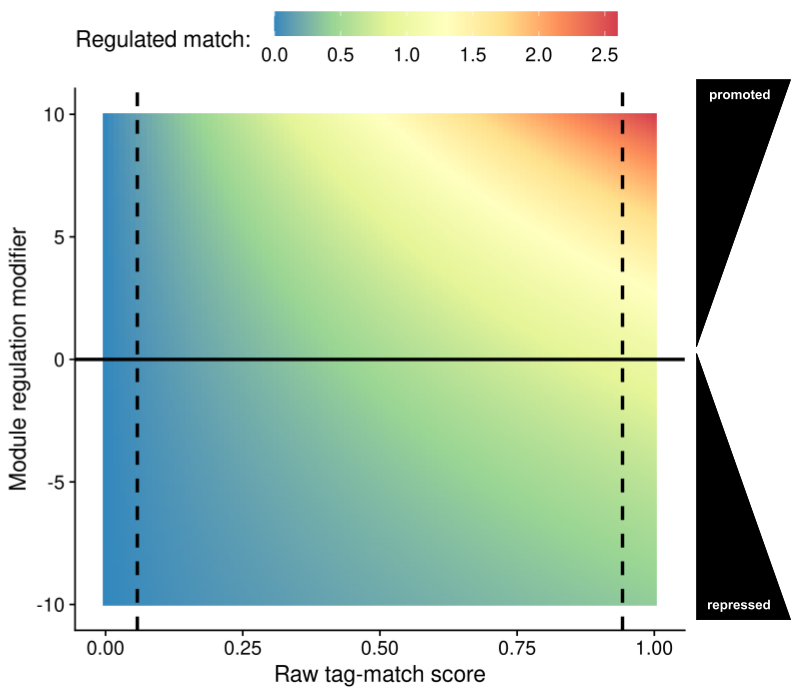
\includegraphics[width=0.6\columnwidth]{chapters/05-tag-based-genetic-regulation/media/expontential-regulation.png}
    \caption{\small
    \textbf{Regulated tag-match score as a function of raw tag-match score and regulatory modifier values according to Equation \ref{chapter:tag-based-regulation:equ:reg-transform}.}
    The horizontal black line indicates a neutral regulatory state; 
    repressed states are below the line, and promoted states are above the line.
    We expect the raw tag-match score (calculated using the Streak similarity metric, which is described later in Section \ref{chapter:tag-based-regulation:sec:methods:signalgp}) of 90\% of random pairs of tags to fall between the two dashed vertical lines; to compute the location of these lines, we generated $10^{5}$ pairs of random tags and found the region that contained the middle 90\% of raw tag-matching scores.
    }
    \label{chapter:tag-based-regulation:fig:exponential-regulation-function}
\end{figure}

When determining which module to reference, each candidate module's $M_r$ is computed, and the module with the highest $M_r$ value is chosen. 
Intuitively, modules with $R_m < 0$ are down-regulated (\textit{i.e.}, in a repressed state), modules with $R_m > 0$ are up-regulated (\textit{i.e.}, in a promoted state), and modules with $R_m = 0$ are unmodified by regulation. 
That is, down-regulated modules have lower tag-match scores than they otherwise would without regulation, and up-regulated modules have higher tag-match scores than they otherwise would without regulation.
Figure \ref{chapter:tag-based-regulation:fig:exponential-regulation-function} gives a visual representation of Equation \ref{chapter:tag-based-regulation:equ:reg-transform}.

In preliminary experiments, we tested several different methods of implementing regulation (including additive, multiplicative, and the current exponential techniques).
We found no evidence for any one method performing substantially better than the others.
Future work will more thoroughly explore the potential effects of different regulation mechanisms. 

\section{Methods}
\label{chapter:tag-based-regulation:sec:methods}

We evaluated how tag-based genetic regulation faculties contribute to, and potentially detract from, the functionality of evolved genetic programs in the context of SignalGP.
First, we assessed the evolvability of our implementation of tag-based genetic regulation: 
can we evolve programs that rely on regulation to dynamically adjust their response to environmental conditions over time? 
Additionally, can tag-based genetic regulation improve problem-solving success on context-dependent problems?
We addressed these questions using the signal-counting and contextual-signal problems, diagnostic tasks that require context-dependent responses to an input signal.

Next, we assessed tag-based genetic regulation on the Boolean-logic calculator problem, a more challenging program synthesis problem that requires programs to perform Boolean logic computations in response to a sequence of input events that represent button presses on a simple calculator. 

% ---- BEGIN REVISION ----
Finally, we used the independent-signal problem to investigate the potential for genetic regulation to impede adaptive evolution by producing maladaptive plasticity. 
The independent-signal problem is a diagnostic that requires programs to associate distinct responses with each type of input; as such, programs do not need to change their response to particular input signals based on prior context.
Additionally, fitness evaluation in the independent-signal problem is imperfect: programs receive input signals in a random order, providing ample opportunity for erroneous regulation to impede adaptive evolution.


% fitness evaluation in the independent-signal problem is imperfect, providing ample opportunity for erroneous regulation to impede adaptive evolution.  

% The changing-signal task does not require programs to contextually change their response to particular inputs, providing ample opportunity for erroneous regulation to impede adaptive evolution.  

% ----- END REVISION ----



\subsection{SignalGP}
\label{chapter:tag-based-regulation:sec:methods:signalgp}

% - High-level overview of SignalGP -
%   - event-driven computing
Here, we provide a general overview of SignalGP; see \citep{lalejini_evolving_2018} for a more in-depth description.
SignalGP defines a scheme for organizing and interpreting genetic programs to afford computational evolution access to the event-driven programming paradigm \citep{cassandras_event-driven_2014}.
In event-driven programs, software execution focuses on processing events (often in the form of messages from other processes, sensor alerts, or user actions).
In SignalGP, events (signals) trigger the execution of program modules (functions), facilitating efficient reactions to exogeneously- or endogeneously-generated signals.
For this work, program modules are represented as sequences of instructions; however, the SignalGP framework generalizes across a variety of program representations \citep{lalejini_what_2019}.

% - Slightly less high-level overview of SignalGP -
%   - organization of programs
%   - tags, tag-based referencing (in signalgp context)
%   - how signals trigger functions
Programs in SignalGP are explicitly modular, comprising a set of functions, each associating a tag with an instruction sequence.
SignalGP makes explicit the concept of events or \textit{signals}.
All signals contain a tag and any associated signal-specific data (\textit{e.g.}, numeric input values).
Because both signals and program functions are tagged, SignalGP determines the most appropriate function to process a signal using tag-based referencing: signals trigger the function with the closest matching tag.

% ------ BEGIN REVISIONS --------
% Comment: Please do two things to add clarity here: 
%  - (1) actually show the equation for the Streak metric, 
%  - (2) clearly define what you mean by "longest contiguously-matching" and "longest contiguously-mismatching". 
%  - For example, are these aligned by index, or are slight misalignments taken into account, for example like Levenshtein string distances? Also, what if two bit strings are identical -- is the mismatch length 0, and then what happens when you divide by 0?

In this work, we represent tags as 256-bit strings, and we quantify the similarity between any two tags using the Streak metric.
The Streak metric was originally proposed by Downing \citep{downing_intelligence_2015} and measures similarity between two bit strings in terms of the relationship between the lengths of the longest contiguously-matching and longest contiguously-mismatching substrings.\footnote{
We make a slight modification to Downing's matching procedure due to an error in its mathematical derivation, as detailed in the supplement \citep{tag_regulation_supplement_2021}.
}
That is, we XOR the two bit strings and count the longest substring of all 0's in the first case or all 1's in the second.
Both our implementation and the mathematical equations for computing the Streak similarity between two bit strings can be found in supplemental material \supSecStreakMetric\ \citep{tag_regulation_supplement_2021}.

% ------ END REVISIONS --------

% ----- BEGIN REVISIONS -----
% -- Signal-driven execution --
When a signal triggers a function, the function executes with the signal's associated data as input.
SignalGP programs can handle many signals simultaneously by processing and responding to each in parallel threads of execution.
Threads each contain local memory registers for performing computations.
Additionally, concurrently executing threads may interact by writing to and reading from a shared global memory buffer.
% @AML: new lines next
For this work, we guaranteed deterministic thread execution using a round robin scheduler to step each thread forward one step (\textit{i.e.}, one instruction) synchronously.

% ----- END REVISIONS -----

% - Instructions -
%   - see supplemental material for full instruction set!
The SignalGP instruction set allows programs to generate internal signals, broadcast external signals, and otherwise work in a tag-based context. 
In this work, each instruction contains one tag and three integer arguments. 
Arguments may modify the effect of an instruction, often specifying memory locations or fixed values.
For example, instructions may refer to and call internal program modules using tag-based referencing; when an instruction generates a signal (\textit{e.g.}, to be used internally or broadcast), the instruction's tag is used as the signal's tag.

%%%%%%%%%%%%%%%%%%%%%%%%%%%%%%%%%%%%%%%%%%%%%%%%%%%%%%%%%%%%%%%%%%%%%%%%%%%%%%%%%%%%%%%%%%%%%%
% Variables to make it easy to change table contents
%%%%%%%%%%%%%%%%%%%%%%%%%%%%%%%%%%%%%%%%%%%%%%%%%%%%%%%%%%%%%%%%%%%%%%%%%%%%%%%%%%%%%%%%%%%%%%

%%%%%%%%%% SetRegulator %%%%%%%%%%
\newcommand{\SetRegulatorName}{\code{SetRegulator+}}
\newcommand{\SetRegulatorArgs}{1}
\newcommand{\SetRegulatorTag}{Yes}
\newcommand{\SetRegulatorDescription}{Set the regulatory modifier of a target module to the value stored in an argument-specified memory register.}

%%%%%%%%%% SetRegulator- %%%%%%%%%%
\newcommand{\SetRegulatorMinusName}{\code{SetRegulator-}}
\newcommand{\SetRegulatorMinusArgs}{1}
\newcommand{\SetRegulatorMinusTag}{Yes}
\newcommand{\SetRegulatorMinusDescription}{Set the regulatory modifier of a target module to the negation of the value stored in an argument-specified memory register.}

\newcommand{\SetOwnRegulatorName}{\code{SetOwnRegulator+}}
\newcommand{\SetOwnRegulatorArgs}{1}
\newcommand{\SetOwnRegulatorTag}{No}
\newcommand{\SetOwnRegulatorDescription}{Set the regulatory modifier of the currently executing module to the value stored in an argument-specified memory register.}

\newcommand{\SetOwnRegulatorMinusName}{\code{SetOwnRegulator-}}
\newcommand{\SetOwnRegulatorMinusArgs}{1}
\newcommand{\SetOwnRegulatorMinusTag}{No}
\newcommand{\SetOwnRegulatorMinusDescription}{Set the regulatory modifier of the currently executing module to the negation of the value stored in an argument-specified memory register.}

\newcommand{\AdjRegulatorName}{\code{AdjRegulator+}}
\newcommand{\AdjRegulatorArgs}{1}
\newcommand{\AdjRegulatorTag}{Yes}
\newcommand{\AdjRegulatorDescription}{Add the value stored in an argument-specified memory register to the regulatory modifier of a target module.}

\newcommand{\AdjRegulatorMinusName}{\code{AdjRegulator-}}
\newcommand{\AdjRegulatorMinusArgs}{1}
\newcommand{\AdjRegulatorMinusTag}{Yes}
\newcommand{\AdjRegulatorMinusDescription}{Subtract the value stored in an argument-specified memory register to the regulatory modifier of a target module.}

\newcommand{\AdjOwnRegulatorName}{\code{AdjOwnRegulator+}}
\newcommand{\AdjOwnRegulatorArgs}{1}
\newcommand{\AdjOwnRegulatorTag}{No}
\newcommand{\AdjOwnRegulatorDescription}{Add the value stored in an argument-specified memory register to the regulatory modifier of the currently executing module.}

\newcommand{\AdjOwnRegulatorMinusName}{\code{AdjOwnRegulator-}}
\newcommand{\AdjOwnRegulatorMinusArgs}{1}
\newcommand{\AdjOwnRegulatorMinusTag}{No}
\newcommand{\AdjOwnRegulatorMinusDescription}{Subtract the value stored in an argument-specified memory-register to the regulatory modifier of the currently executing module.}

\newcommand{\ClearRegulatorName}{\code{ClearRegulator}}
\newcommand{\ClearRegulatorArgs}{0}
\newcommand{\ClearRegulatorTag}{Yes}
\newcommand{\ClearRegulatorDescription}{Reset the regulatory modifier of a target module.}

\newcommand{\ClearOwnRegulatorName}{\code{ClearOwnRegulator}}
\newcommand{\ClearOwnRegulatorArgs}{0}
\newcommand{\ClearOwnRegulatorTag}{No}
\newcommand{\ClearOwnRegulatorDescription}{Reset the regulatory modifier of the currently executing module.}

\newcommand{\SenseRegulatorName}{\code{SenseRegulator}}
\newcommand{\SenseRegulatorArgs}{1}
\newcommand{\SenseRegulatorTag}{Yes}
\newcommand{\SenseRegulatorDescription}{Load the value of a target module's regulatory modifier into an argument-specified memory register.}

\newcommand{\SenseOwnRegulatorName}{\code{SenseOwnRegulator}}
\newcommand{\SenseOwnRegulatorArgs}{1}
\newcommand{\SenseOwnRegulatorTag}{No}
\newcommand{\SenseOwnRegulatorDescription}{Load the value of the currently executing module's regulatory modifier into an argument-specified memory register.}

\newcommand{\IncRegulatorName}{\code{IncRegulator}}
\newcommand{\IncRegulatorArgs}{0}
\newcommand{\IncRegulatorTag}{Yes}
\newcommand{\IncRegulatorDescription}{Add one to the regulatory modifier of a target module. }

\newcommand{\IncOwnRegulatorName}{\code{IncOwnRegulator}}
\newcommand{\IncOwnRegulatorArgs}{0}
\newcommand{\IncOwnRegulatorTag}{No}
\newcommand{\IncOwnRegulatorDescription}{Add one to the regulatory modifier of the currently executing module.}

\newcommand{\DecRegulatorName}{\code{DecRegulator}}
\newcommand{\DecRegulatorArgs}{0}
\newcommand{\DecRegulatorTag}{Yes}
\newcommand{\DecRegulatorDescription}{Subtract one from the regulatory modifier of a target module.}

\newcommand{\DecOwnRegulatorName}{\code{DecOwnRegulator}}
\newcommand{\DecOwnRegulatorArgs}{0}
\newcommand{\DecOwnRegulatorTag}{No}
\newcommand{\DecOwnRegulatorDescription}{Subtract one from the regulatory modifier of the currently executing module.}

%%%%%%%%%%%%%%%%%%%%%%%%%%%%%%%%%%%%%%%%%%%%%%%%%%%%%%%%%%%%%%%%%%%%%%%%%%%%%%%%%%%%%%%%%%%%%%
% Table
%%%%%%%%%%%%%%%%%%%%%%%%%%%%%%%%%%%%%%%%%%%%%%%%%%%%%%%%%%%%%%%%%%%%%%%%%%%%%%%%%%%%%%%%%%%%%%

\begin{table}[htbp]
    \small
    \centering
    \begin{tabular}{l | p{0.6\columnwidth}}
        \toprule
        \textbf{Instruction} & 
        % Args. & 
        % Tag-based? & 
        \textbf{Description} 
        \\ \hline 
        
        \SetRegulatorName & 
        % \SetRegulatorArgs & 
        % \SetRegulatorTag & 
        \SetRegulatorDescription 
        \\ \hline
        
        \SetRegulatorMinusName & 
        % \SetRegulatorMinusArgs & 
        % \SetRegulatorMinusTag & 
        \SetRegulatorMinusDescription 
        \\ \hline
        
        \SetOwnRegulatorName &
        % \SetOwnRegulatorArgs &
        % \SetOwnRegulatorTag &
        \SetOwnRegulatorDescription 
        \\ \hline
        
        \SetOwnRegulatorMinusName & 
        % \SetOwnRegulatorMinusArgs & 
        % \SetOwnRegulatorMinusTag & 
        \SetOwnRegulatorMinusDescription 
        \\ \hline
        
        \AdjRegulatorName & 
        % \AdjRegulatorArgs & 
        % \AdjRegulatorTag & 
        \AdjRegulatorDescription 
        \\ \hline
        
        \AdjRegulatorMinusName & 
        % \AdjRegulatorMinusArgs & 
        % \AdjRegulatorMinusTag & 
        \AdjRegulatorMinusDescription 
        \\ \hline
        
        \AdjOwnRegulatorName & 
        % \AdjOwnRegulatorArgs & 
        % \AdjOwnRegulatorTag & 
        \AdjOwnRegulatorDescription 
        \\ \hline
        
        \AdjOwnRegulatorMinusName & 
        % \AdjOwnRegulatorMinusArgs & 
        % \AdjOwnRegulatorMinusTag &
        \AdjOwnRegulatorMinusDescription 
        \\ \hline
        
        \ClearRegulatorName & 
        % \ClearRegulatorArgs & 
        % \ClearRegulatorTag & 
        \ClearRegulatorDescription 
        \\ \hline
        
        \ClearOwnRegulatorName & 
        % \ClearOwnRegulatorArgs & 
        % \ClearOwnRegulatorTag & 
        \ClearOwnRegulatorDescription
        \\ \hline
        
        \SenseRegulatorName & 
        % \SenseRegulatorArgs & 
        % \SenseRegulatorTag & 
        \SenseRegulatorDescription 
        \\ \hline
        
        \SenseOwnRegulatorName & 
        % \SenseOwnRegulatorArgs & 
        % \SenseOwnRegulatorTag & 
        \SenseOwnRegulatorDescription
        \\ \hline
        
        \IncRegulatorName & 
        % \IncRegulatorArgs & 
        % \IncRegulatorTag & 
        \IncRegulatorDescription 
        \\ \hline
        
        \IncOwnRegulatorName & 
        % \IncOwnRegulatorArgs & 
        % \IncOwnRegulatorTag & 
        \IncOwnRegulatorDescription 
        \\ \hline
        
        \DecRegulatorName & 
        % \DecRegulatorArgs & 
        % \DecRegulatorTag & 
        \DecRegulatorDescription 
        \\ \hline
        
        \DecOwnRegulatorName & 
        % \DecOwnRegulatorArgs & 
        % \DecOwnRegulatorTag & 
        \DecOwnRegulatorDescription
        \\ 
        \bottomrule
    \end{tabular}
    \caption{\small 
    \textbf{Regulatory instructions used in this work.} 
    We include (+) and (-) instruction variants to ensure that positive and negative regulation values are equally probable.
    }
    \label{chapter:tag-based-regulation:tab:regulation-instructions}
\end{table}


% regulation in signalgp
Previous work has demonstrated that SignalGP facilitates the evolution of event-driven programs capable of identifying and responding to many \textit{distinct} signals \citep{lalejini_what_2019}.
% However, without access to regulation, SignalGP requires programs to use procedural mechanisms (\textit{e.g.}, if statements) to adjust how they respond to a particular signal over time.
However, without access to regulation, SignalGP requires programs to track context in memory and use procedural mechanisms (\textit{e.g.}, if statements) to adjust how they respond to a particular signal over time based on stored context.
Here, we apply tag-based genetic regulation to SignalGP (as described in Section \ref{chapter:tag-based-regulation:sec:tag-based-genetic-regulation}).
We supplemented the instruction set with regulatory instructions (Table \ref{chapter:tag-based-regulation:tab:regulation-instructions}) that use tag-based referencing to target internal functions. 
In this work, we apply regulation to function references using Equation \ref{chapter:tag-based-regulation:equ:reg-transform}. 
Our full instruction set, including descriptions of each instruction, can be found in our supplemental material \citep{tag_regulation_supplement_2021}.

\subsubsection{Evolution}

In this work, we propagated programs asexually, and we applied mutations to offspring.
The parent-selection method varied across experiments.
Programs were variable-length: each program contained up to \MaxFuncCnt\ modules, and each module contained up to \MaxFuncInstCnt\ instructions.

% ---- BEGIN REVISION -----

We applied single-instruction substitution, insertion, and deletion mutations each at a per-instruction rate of \MutRateInstPoint. 
Additionally, we applied a `slip' mutation operator \citep{lalejini_gene_2017} that could duplicate or delete entire sequences of instructions at a per-module rate of \MutRateSeqSlip. 
We mutated numeric instruction arguments at a per-argument rate of \MutRateInstArgSub, and we limited numeric arguments to values between \MinArgValue\ and \MaxArgValue.
When a numeric argument mutated, we randomized the argument's value to a valid integer between \MinArgValue\ and \MaxArgValue.
We mutated instruction- and module-tags at a per-bit rate of \MutRateTagBF.
We applied whole-module duplication and deletion operators at a per-module rate of \MutRateFuncDup, allowing the number of modules in a program to evolve.

% ---- END REVISION -----

% \subsection{Repeated-signal Problem}
% \label{sec:methods:repeated-signal-problem}
\subsection{Signal-counting Problem}
\label{chapter:tag-based-regulation:sec:methods:signal-counting-problem}

% ----- BEGIN REVISION -----
% - Issue: does a program simply have to execute the corresponding Response-i instruction, or do the Response-i instructions output some other value? I think the former, but this could be clearer.
The signal-counting problem requires programs to continually change their response to an environmental signal, producing the appropriate output each of the $K$ times that signal is repeated.
Programs output responses by executing one of $K$ response instructions. 
For example, if a program receives two signals from the environment during evaluation (\textit{i.e.}, $K=2$), the program should execute \code{Response-1} after the first signal and \code{Response-2} after the second signal; aside from executing the correct response instruction, no other output is necessary after receiving an environmental signal.

% ----- END REVISION -----

% ----- BEGIN REVISION -----
% - Issue: what is a time step?
We provide programs \RepeatSigTaskCpuTimePerSignal\ time steps to respond to each environmental signal.
% @AML: new sentence next
During each time step, each of a program's active thread's execute a single instructions.
Once the allotted time expires or the program outputs a response, the program's threads of execution reset, resulting in a loss of all thread-local memory; \textit{only} the contents of the global memory buffer and each program module's regulatory state persist.
The environment then produces the next signal (identical to each previous environmental signal) to which the program may respond.
A program \textit{must} use the global memory buffer or genetic regulation to correctly shift its response to each subsequent environmental signal. 
Evaluation continues in this way until the program correctly responds to each of the $K$ environmental signals or until the program executes an incorrect response.
A program's fitness equals the number of consecutive correct responses given during evaluation, and a program is considered a solution if it correctly responds to all $K$ environmental signals.

% ----- END REVISION ----

\subsubsection{Experimental Design}

The signal-counting problem is explicitly designed to 
(1) evaluate if tag-based genetic regulation can be evolved to dynamically adjust which modules execute in response to a \textit{repeated} input type 
and (2) assess the problem-solving success of a regulation-enabled GP system relative to an otherwise identical GP system with regulation disabled. 
We compared programs evolved in a regulation-on treatment to those evolved in a regulation-off control.
In the control treatment, we used an identical instruction set where regulation instructions were altered to behave as no-operation instructions.  As such, programs must use global memory (in combination with procedural flow-control mechanisms) to correctly respond to environmental signals.

For each experimental condition, we evolved 200 replicate populations of 1000 programs for 10,000 generations at four levels of problem difficulty: $K=2, 4, 8$, and 16.
For each replicate, we randomly generated a unique tag for each environmental signal, and we initialized populations with randomly generated programs.
Each generation, we evaluated programs independently, and we selected programs using size-eight tournament selection.

\subsection{Contextual-signal Problem}
\label{chapter:tag-based-regulation:sec:methods:contextual-signal-problem}

The contextual-signal problem is inspired by Skocelas and DeVries' method for verifying the functionality of recurrent neural network implementations \citep{skocelas_test_2020}. 
In the contextual-signal problem, programs must respond appropriately to a pair of input signals.
The order of these signals does not matter, but the first signal must be remembered (as ``context'') in order to produce the correct response to the second signal.
In this work, there are a total of four possible input signals and four possible outputs.
Programs output a particular response by executing one of four response instructions. 
Table \ref{chapter:tag-based-regulation:tab:context-signal-input-combos} gives the correct output type for each pairing of input signals. 


\begin{table}[h!]
    \small
    \centering
    \begin{tabular}{c | c | c}
        \toprule
        Test case ID & Input Sequence & Correct Response \\ \hline 
        0 &
        S-0, S-0 &
        Response-A \\ 
        % \hline
        1 &
        S-0, S-1 &
        Response-B \\  
        % \hline
        2 &
        S-0, S-2 &
        Response-C \\  
        % \hline
        3 &
        S-0, S-3 &
        Response-D \\ 
        % \hline
        
        4 &
        S-1, S-0 &
        Response-B \\ 
        % \hline
        5 &
        S-1, S-1 &
        Response-C \\ 
        % \hline
        6 &
        S-1, S-2 &
        Response-D \\ 
        % \hline
        7 &
        S-1, S-3 &
        Response-A \\ 
        % \hline
        
        8 &
        S-2, S-0 &
        Response-C \\ 
        % \hline
        9 &
        S-2, S-1 &
        Response-D \\ 
        % \hline
        10 &
        S-2, S-2 &
        Response-A \\ 
        % \hline
        11 &
        S-2, S-3 &
        Response-B \\ 
        % \hline
        
        12 &
        S-3, S-0 &
        Response-D \\ 
        % \hline
        13 &
        S-3, S-1 &
        Response-A \\ 
        % \hline
        14 &
        S-3, S-2 &
        Response-B \\ 
        % \hline
        15 &
        S-3, S-3 &
        Response-C \\ 
        \bottomrule
    \end{tabular}
    \caption{\small 
    \textbf{Input signal sequences for the contextual-signal problem.} 
    }
    \label{chapter:tag-based-regulation:tab:context-signal-input-combos}
\end{table} 

We evaluate programs on each of the 16 possible sequences of input signals (Table \ref{chapter:tag-based-regulation:tab:context-signal-input-combos}); we consider each of these input sequences as a single test case.
For each test case evaluation, we give programs \ContextSigTaskCpuTimePerSignal\ time steps to process each signal.
After the first input signal, a program must update internal state information to ensure that the second input signal induces the correct response.  
Once the allotted time expires after the first input signal, the program's threads of execution are reset, resulting in a loss of all thread-local memory; \textit{only} the contents of global memory and each function's regulatory state persist. 
The program then receives the second input signal and must execute the correct response instruction within \ContextSigTaskCpuTimePerSignal\ time steps.
A program is considered a solution if it produces the correct response for all 16 possible sequences of input signals.

\subsubsection{Experimental Design}

We use the contextual-signal problem to
(1) assess the capacity of tag-based genetic regulation to perform context-dependent module execution based on \textit{distinct} input types
and
(2) evaluate the problem-solving success of a regulation-enabled GP system relative to an otherwise identical GP system with regulation disabled.
As in the signal-counting problem, we compared the problem-solving success of regulation-on and regulation-off GP systems.

For each experimental condition, we evolved 200 replicate populations of 1000 programs for 10,000 generations.
For each replicate, we randomly generated the tags associated with each type of input signal, and we initialized populations with randomly generated programs.
Instead of selecting programs to propagate based on an aggregate fitness measure, we used the lexicase parent selection algorithm \citep{helmuth_solving_2015} in which each combination of input signals (\textit{i.e}., row in Table \ref{chapter:tag-based-regulation:tab:context-signal-input-combos}) constituted a single test case. 

\subsection{Boolean-logic Calculator Problem}
\label{chapter:tag-based-regulation:sec:methods:boolean-calc-problem}
% alternative names
% - Bitwise Logic Calculator Problem

Inspired by Yeboah-Antwi's PushCalc system \citep{yeboah-antwi_evolving_2012}, 
the Boolean-logic calculator problem requires programs to implement a push-button calculator capable of performing each of the following 10 bitwise logic operations: ECHO, NOT, NAND, AND, OR-NOT, OR, AND-NOT, NOR, XOR, and EQUALS. 
Table \ref{chapter:tag-based-regulation:tab:boolean-calc-operations} gives a brief overview of each of these operations. 
In this problem, there are 11 distinct types of input signals: one for each of the 10 possible operators and one for numeric inputs. 
Each distinct signal type is associated with a unique tag (randomly generated per-replicate) and is meant to recreate the context that must be maintained on a physical calculator.
Programs receive a sequence of input signals in prefix notation, starting with an operator signal and followed by the appropriate number of numeric input signals (that each contain an operand to use in the computation).
After receiving the appropriate input signals, programs must output the correct result of the requested computation.

% http://myxo.css.msu.edu/papers/nature2003/Supp2.html

\begin{table}[ht!]
    \small
    \centering
    \begin{tabular}{c | c | c}
        \toprule
        Operation & \# Inputs & NAND gates \\ \hline 
        ECHO &
        1 &
        0
        \\
        NOT &
        1 &
        1
        \\
        NAND &
        2 &
        1
        \\
        AND &
        2 &
        2
        \\
        OR-NOT &
        2 &
        2
        \\
        OR &
        2 &
        3
        \\
        AND-NOT &
        2 &
        3
        \\
        NOR &
        2 &
        4
        \\
        XOR &
        2 &
        4
        \\
        EQUALS &
        2 &
        5
        \\
        \bottomrule
    \end{tabular}
    \caption{\small 
    \textbf{Bitwise Boolean logic operations used in the Boolean-logic calculator problem.} 
    Programs are given a \code{nand} instruction and must construct each of the other operations (aside from ECHO) out of \code{nand} operations.
    As such, we measure the difficulty of each operation as the minimum number of NAND gates required to construct the given operation.
    }
    \label{chapter:tag-based-regulation:tab:boolean-calc-operations}
\end{table}

Programs are evaluated on a set of test cases (\textit{i.e.}, input/output examples) where each test case comprises a particular operator, the requisite number of operands, and the expected numeric output.
Test cases are evaluated on a pass/fail basis, and a program is classified as a solution if it passes all test cases in a training and testing set\footnote{
We use the testing set only to determine if a program can be categorized as a solution. The testing set is never used by the parent-selection algorithm to determine reproductive success.
}.
The training and testing sets used in this work are included in our supplemental material \citep{tag_regulation_supplement_2021} and contained 442 and 5810 test cases, respectively.
Each generation, we sample 20 test cases from the training set, and we independently evaluate each program in the population on the sampled test cases.

When evaluating a program on a test case, we provide \CalculatorTaskCpuTimePerSignal\ time steps to process each input signal.
After time expires, the program's threads of execution are reset, resulting in a loss of all thread-local memory; only the contents of global memory and each function's regulatory state persist.
Because input-signals are given in prefix notation, programs must adjust their internal state to ensure that the program performs and outputs the result of the appropriate computation after receiving the requisite number of operand input signals.

% # training cases: 442
% # testing cases: 5810
% # total cases: 6252
% Number of training examples to evaluate each generation: 20
%   Test case type: NOR; TypeID: 9; # training cases: 45; # training sample eval: 2
%   Test case type: ANDNOT; TypeID: 8; # training cases: 45; # training sample eval: 2
%   Test case type: XOR; TypeID: 7; # training cases: 45; # training sample eval: 2
%   Test case type: NOT; TypeID: 6; # training cases: 41; # training sample eval: 2
%   Test case type: ECHO; TypeID: 5; # training cases: 41; # training sample eval: 2
%   Test case type: EQU; TypeID: 1; # training cases: 45; # training sample eval: 2
%   Test case type: NAND; TypeID: 0; # training cases: 45; # training sample eval: 2
%   Test case type: ORNOT; TypeID: 2; # training cases: 45; # training sample eval: 2
%   Test case type: AND; TypeID: 3; # training cases: 45; # training sample eval: 2
%   Test case type: OR; TypeID: 4; # training cases: 45; # training sample eval: 2


\subsubsection{Experimental Design}

We use the Boolean-logic calculator problem to assess the utility of tag-based regulation on a challenging program synthesis problem. 
The signal-counting and contextual-signal problems each require programs to perform different computations in response to input signals, but those computations are abstracted as `response' instructions. 
The Boolean-logic calculator problem requires programs to both dynamically adjust which modules are executed in response to input signals and perform non-trivial computations on numeric inputs. 

We compared the problem-solving success of programs evolved in regulation-on and regulation-off conditions.
For each condition, we evolved 200 replicate populations of 1000 programs for 10,000 generations.
For each replicate, we randomly generated the tags associated with each type of input signal, and we initialized populations with randomly generated programs.
We selected parents using a variant of the down-sampled lexicase algorithm \citep{hernandez_random_2019}, guaranteeing that at least one of each type of test case (\textit{i.e.}, at least one of each type of operator) was used during evaluation. 

\subsection{Independent-signal Problem}
\label{chapter:tag-based-regulation:sec:methods:independent-signal-problem}

% ----- BEGIN REVISION -----

The independent-signal problem requires programs to execute a unique response for each of 16 distinct input signals. 
Because signals are distinct, programs need not alter their response to any particular signal over time.
Instead, programs may ``hardwire'' each of the 16 possible responses to the appropriate input signal.
However, input signals are presented in a random order; thus, the correct \textit{order} of responses cannot be hardcoded.
Otherwise, evaluation (and fitness assignment) on the independent-signal task mirrors that of the signal-counting task (Section \ref{chapter:tag-based-regulation:sec:methods:signal-counting-problem}).
A program is considered a solution if it responds correctly to all 16 input signals during evaluation.

\subsubsection{Experimental Design}

%%% @AML: working on highlighting how fitness eval is deliberately imperfect.
% - Problems of this nature are common: robot simulations, or large input spaces where only possible to test on small sample of input types. 
We deliberately configured fitness evaluation and solution identification in the independent-signal problem to be noisy: each program is evaluated once on a single random ordering of input signals, and we label a program as a solution if it performs optimally during a single evaluation.
Because programs receive input signals in a random order, erroneous genetic regulation can manifest as cryptic variation (\textit{i.e.}, behavioral variation that is not expressed and selected on).
For example, non-adaptive down-regulation of a particular response-function may be neutral given one sequence of input signals, but may be deleterious in another.
Indeed, this form of non-adaptive cryptic variation can also result from erroneous flow control structures. 

The independent-signal problem allows us to test whether genetic regulation can impede adaptive evolution in scenarios where outputs are not context-dependent and where fitness evaluation does not reliably differentiate between generalizing and non-generalizing candidate solutions.
Fitness evaluation for the independent-signal problem is computationally inexpensive, so we could easily increase the reliability of evaluation by testing programs on multiple orderings of input sequences.
However, our goal is not to demonstrate that we can \textit{solve} this simple diagnostic problem.
Rather, we aim to determine if this diagnostic represents a general scenario where unnecessary tag-based regulation can impede adaptive evolution relative to not having regulation. %, [as many real-world problems are likely to have unreliable evaluation (\textit{e.g.}, robotics simulations, [...]).]
% The changing-signal problem assesses the potential for unnecessary tag-based genetic regulation to \textit{impede} adaptive evolution relative to not having regulation.

As in each of the previous experiments, we compared programs evolved in regulation-on and regulation-off conditions.
Specifically, we compared initial problem-solving success and how well solutions generalized to a sample of 5000 input sequences (of ${\sim}2.1\times10^{13}$ possible sequences). 
We deemed programs as having generalized only if they responded correctly in all 5000 tests.

We evolved 200 replicate populations of 1000 programs for 10,000 generations under each condition. 
For each replicate, we randomly generated 16 unique input signal tags.
All other experimental procedures were identical to that of the signal-counting task.

% ------ END REVISION ------

\subsection{Data Analysis and Reproducibility}

% How knockout experiments work
For each replicate in a given experiment, we extracted and analyzed the first evolved program that was classified as a solution. 
We compared the number of successful replicates (\textit{i.e.}, replicates that yielded a solution) across experimental conditions using Fisher's exact test.
%, and we applied a Bonferroni correction for multiple comparisons where appropriate. %@AML: no actual multiple comparisons in results!
We conducted knockout experiments on successful programs to identify the mechanisms underlying their behavior.
In all knockout experiments, we re-evaluated programs with a target functionality (\textit{e.g.}, regulation instructions) replaced with no-operation instructions.
Specifically, we independently knocked out (1) all regulatory instructions, (2) all instructions that access a program's global memory buffer, and (3) both regulatory instructions and global memory access instructions. 
We classify a program as reliant on a particular functionality if, when knocked out, fitness decreases. 
In addition to knockout experiments, we tracked the distribution of instruction types (\textit{e.g.}, flow control, mathematical operations, \textit{etc.}) executed by successful programs. 
For each successful replicate, we extracted the proportion of flow control instructions (\textit{i.e.}, conditional logic instructions such as ``if'' or ``while'' statements) executed by the evolved solution. 
We compared the proportions of flow control instructions executed by regulation-on solutions and regulation-off solutions, allowing us to assess the relative importance of conditional logic across experimental treatments.

For programs reliant on genetic regulation, we abstracted regulatory networks as directed graphs by monitoring program execution.
Vertices represent program functions, and directed edges (each categorized as promoting or repressing) show the regulatory interactions between two functions.
For example, a repressing edge from function A to function B indicates that B was repressed when A was executing.

We implemented our experiments using the Empirical scientific software library \citep{charles_ofria_2020_empirical}, and we conducted all statistical analyses using R version 4.0.2 \citep{r_language_2020}.
We used the reshape2 \cite{R-reshape2} R package and the tidyverse \citep{r_tidyverse_2019} collection of R packages to wrangle data. 
We used the following R packages for graphing and visualization: ggplot2 \citep{R-ggplot2}, cowplot \citep{R-cowplot}, viridis \citep{R-viridis}, Color Brewer \citep{harrower_colorbrewerorg_2003,R-Brewer_2014}, and igraph \citep{igraph2006}.
We used R markdown \citep{rmarkdown} and bookdown \citep{R-bookdown} to generate web-enabled supplemental material.
Our source code for experiments and analyses, along with guides for replication, can be found in supplemental material \citep{tag_regulation_supplement_2021}, which is hosted on \href{https://github.com/amlalejini/Tag-based-Genetic-Regulation-for-LinearGP/}{GitHub}\footnote{\url{https://github.com/amlalejini/Tag-based-Genetic-Regulation-for-LinearGP/}}.
Additionally, we have made all of our experimental data available on the \href{https://osf.io/928fx/}{Open Science Framework} (see \supSecDataAvailability\ in supplement \citep{tag_regulation_supplement_2021}).

\section{Results and Discussion}

\begin{raggedright}
\subsection{Tag-based regulation improves problem-solving performance on context-dependent tasks}
\end{raggedright}

% Overview paragraph (outline results across all three context-dependent problems)
We found that tag-based regulation improves performance on each of the three problems that require context-dependent behavior: the signal-counting problem (Section \ref{chapter:tag-based-regulation:sec:results:signal-counting-problem}), contextual-signal problem (Section \ref{chapter:tag-based-regulation:sec:results:context-signal-problem}), and Boolean-logic calculator problem (Section \ref{chapter:tag-based-regulation:sec:results:boolean-calc-problem}). 
Additionally, we conducted knockout experiments that confirmed that evolved tag-based regulation allows solutions to dynamically adjust module execution over time. 
We also found that, across all three context-dependent problems, regulation-off solutions (\textit{i.e.}, solutions evolved using regulation-disabled SignalGP) executed a larger proportion of conditional logic instructions than regulation-on solutions (\textit{i.e.}, solutions evolved using regulation-enabled SignalGP). 
This result suggests that without regulation, programs must evolve larger, more complex conditional logic structures. 

\subsubsection{Signal-counting Problem}
\label{chapter:tag-based-regulation:sec:results:signal-counting-problem}


\begin{table}[ht!]
    \small
    \centering
    \begin{tabularx}{\columnwidth}{cYY}
        \toprule
          & Regulation-off condition 
          & Regulation-on condition \\
        %  \hline
        \cmidrule(lr){1-3}
         Two-signal   
            & \RSPTwoSigMemOnlySolutionCnt  % Memory-only
            & \RSPTwoSigBothSolutionCnt \\  % Both
        %  \hline
         Four-signal
            & \RSPFourSigMemOnlySolutionCnt  % Memory-only
            & \RSPFourSigBothSolutionCnt \\  % Both
        %  \hline
         Eight-signal 
            & \RSPEightSigMemOnlySolutionCnt  % Memory-only
            & \RSPEightSigBothSolutionCnt \\  % Both
        %  \hline
         Sixteen-signal
            & \RSPSixteenSigMemOnlySolutionCnt  % Memory-only
            & \RSPSixteenSigBothSolutionCnt \\  % Both
         \bottomrule
    \end{tabularx}
    \caption{\small
    \textbf{Signal-counting problem-solving success.}
    This table gives the number of successful replicates (\textit{i.e.}, in which a perfect solution evolved) out of 200 on the signal-counting problem across four problem difficulties and two experimental conditions. 
    For each problem difficulty, the regulation-off condition was less successful than the regulation-on condition (Fisher's exact test; all difficulties: $p < 10^{-15}$).
    }
    \label{chapter:tag-based-regulation:tab:signal-counting-solutions}
\end{table}


% two-signal: p-value < 2.2e-16, 
% four-signal: p-value < 2.2e-16
% eight-signal: p-value < 2.2e-16
% sixteen-signal: p-value < 2.2e-16

% (1) # Solution & solution timing
Table \ref{chapter:tag-based-regulation:tab:signal-counting-solutions} shows the results from the signal-counting problem for each experimental condition across all four levels of problem difficulty. 
Regulation-on conditions consistently yielded a larger number of successful replicates than regulation-off conditions where programs relied on their global memory buffer in combination with procedural flow control for success.
Although global memory is technically sufficient to solve each version of the signal-counting problem\footnote{
We verified this claim by hand-coding solutions that rely on global memory and flow-control instructions (supplemental \supSecHandcodedPrograms\ \citep{tag_regulation_supplement_2021}).
}, 
in practice such solutions evolved in only the two- and four-signal variants.
Tag-based regulation, in contrast, appears more readily adaptive, as regulation-based solutions arose across all problem difficulties, implying that access to tag-based regulation can drive increased problem-solving success.
Further, we found that, in the two- and four-signal tasks, solutions arose after significantly fewer generations in the regulation-on conditions than in the regulation-off controls (Figure \ref{chapter:tag-based-regulation:fig:signal-counting-solve-time}).


\begin{figure}[htbp]
    \centering
    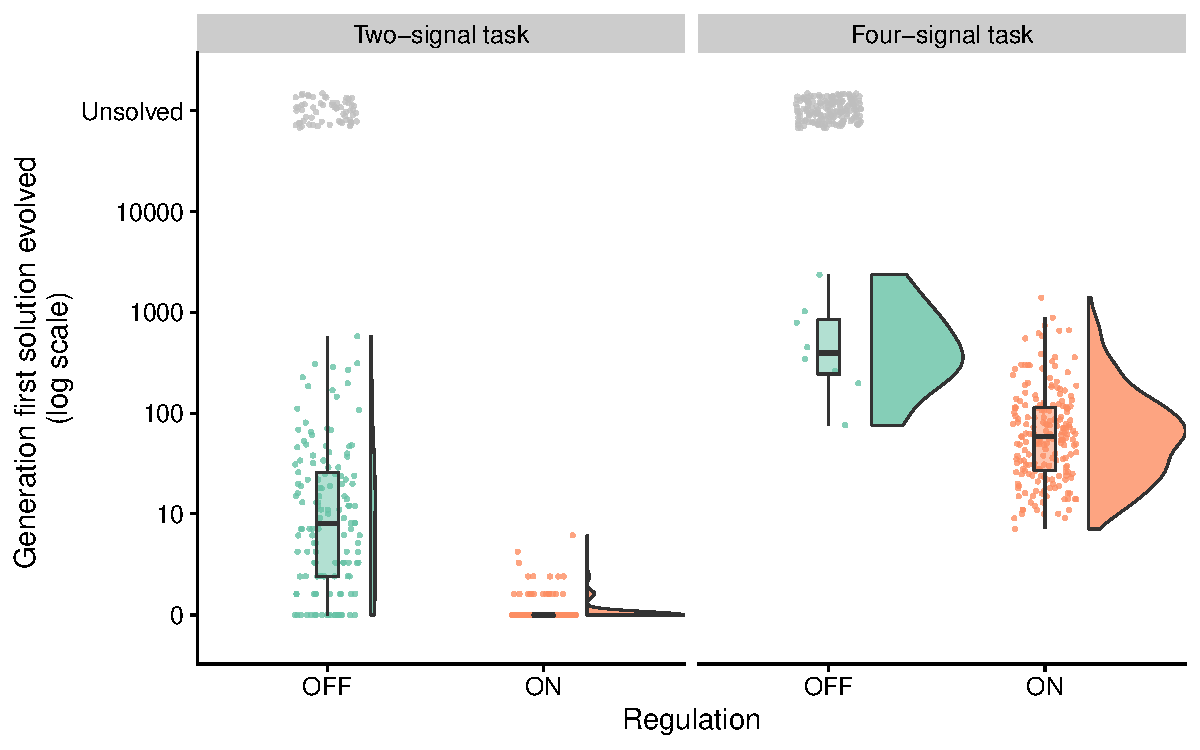
\includegraphics[width=0.7\textwidth]{chapters/05-tag-based-genetic-regulation/media/signal-counting-solve-time-cloud.pdf}
    \caption{\small
    \textbf{Generation at which first solution evolved (log scale) in each successful replicate for the signal-counting problem (raincloud plot \citep{allen_raincloud_2019}).}
    We show data from only those problem difficulties in which solutions evolved (two- and four-signal problems).
    Gray points indicate the number of unsuccessful replicates for each condition.
    For both problem difficulties, regulation-on solutions typically required fewer generations than regulation-off solutions to arise (Wilcoxon rank sum test; two-signal: $p < 10^{-15}$, four-signal: $p < 9\times10^{-05}$). 
    }
    \label{chapter:tag-based-regulation:fig:signal-counting-solve-time}
\end{figure}

% two-signal - p-value < 2.2e-16
% four-signal 8.603e-05

Tag-based regulation renders the two-signal task trivial: all solutions evolved in under 10 generations. 
In fact, the majority of regulation-on solutions (178 out of 200) were found in the initial randomly generated population. 
However, not all replicates without access to tag-based regulation even found a solution to the two-signal task.

\begin{table}[htbp]
    \small
    \centering
    \begin{tabularx}{\columnwidth}{cYYY}
        \toprule
          & No regulation required
          & Regulation required 
          & Unsolved \\
        %  \hline
        \cmidrule(lr){1-4}
         Two-signal     
            & \RSPTwoSigMemOnlyStrategyCnt  % Memory-only
            & \RSPTwoSigRegRequiredStrategyCnt  
            & \RSPTwoSigUnsolvedCnt \\
        %  \hline
         Four-signal    
            & \RSPFourSigMemOnlyStrategyCnt  % Memory-only
            & \RSPFourSigRegRequiredStrategyCnt   % 
            & \RSPFourSigUnsolvedCnt \ \\
        %  \hline
         Eight-signal   
            & \RSPEightSigMemOnlyStrategyCnt  % Memory-only
            & \RSPEightSigRegRequiredStrategyCnt  % 
            & \RSPEightSigUnsolvedCnt \\
        %  \hline
         Sixteen-signal 
            & \RSPSixteenSigMemOnlyStrategyCnt  % Memory-only
            & \RSPSixteenSigRegRequiredStrategyCnt  % 
            & \RSPSixteenSigUnsolvedCnt \\
         \bottomrule
    \end{tabularx}
    \caption{\small 
    \textbf{Mechanisms underlying solutions from the regulation-on condition for the signal-counting problem.}
    To determine a successful program's underlying strategy, we re-evaluated the program with global memory access instructions knocked out (\textit{i.e.}, replaced with no-operation instructions) and with regulation instructions knocked out.
    This table shows the number of regulation-on solutions that actually rely on regulation to solve the signal-counting problem. 
    }
    \label{chapter:tag-based-regulation:tab:signal-counting-ko-strategies}
\end{table} 

We conducted knockout experiments to investigate the mechanisms underlying successful programs. 
Indeed, all solutions evolved without access to tag-based regulation relied exclusively on their global memory buffer to differentiate their behavior (see supplemental \supSecRepeatedSigAnalysis\ \citep{tag_regulation_supplement_2021}). 
Table \ref{chapter:tag-based-regulation:tab:signal-counting-ko-strategies} shows the strategies used by programs evolved with regulation-enabled SignalGP.
Our knockout experiments confirm that the majority of solutions evolved with access to tag-based regulation do indeed rely on regulation to dynamically adjust their responses to signals over time. 


\begin{figure}[ht]
\centering

\begin{subfigure}[b]{0.55\textwidth}
    \centering
    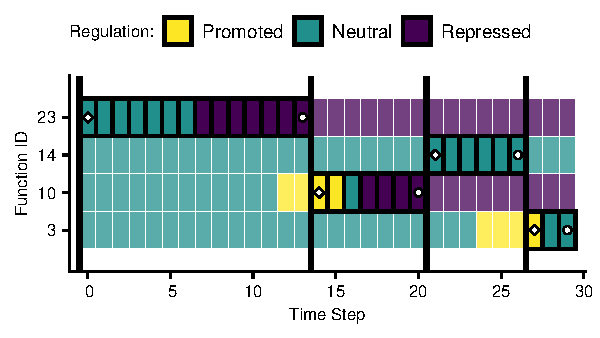
\includegraphics[width=\linewidth]{chapters/05-tag-based-genetic-regulation/media/signal-counting-networks/case-study-trace-id-20203-regulator-state-horizontal.pdf}
    \caption{\small Module regulation over time.}
    \label{chapter:tag-based-regulation:subfig:rst-exec-trace}
\end{subfigure}%
\hfill
\begin{subfigure}[b]{0.3\textwidth}
    \centering
    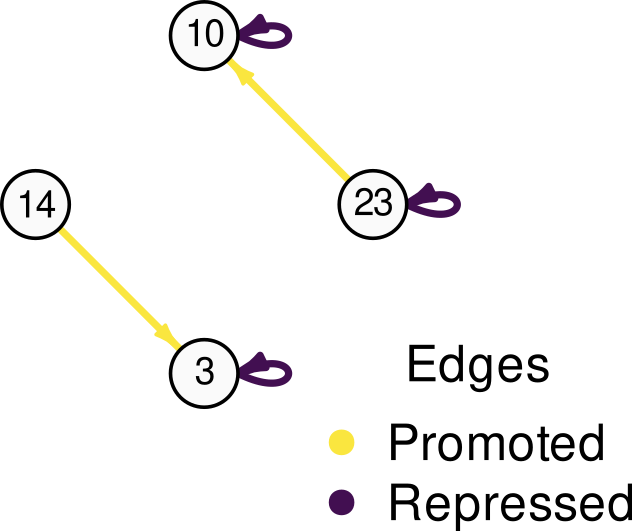
\includegraphics[width=\linewidth]{chapters/05-tag-based-genetic-regulation/media/signal-counting-networks/case-study-id-20203-network.png}
    \caption{\small Regulatory network.}
    \label{chapter:tag-based-regulation:subfig:rst-reg-network}
\end{subfigure}%


\caption{\small 
   \textbf{Execution trace of a SignalGP program solving the four-signal version of the signal-counting task.}
    Color denotes each function's regulatory state (yellow: promoted, purple: repressed) during evaluation; functions not regulated or executed are omitted.
    Functions that are actively executing are annotated with a black outline.
    Black vertical lines denote input signals, and a diamond (white with black outline) indicates which function was triggered by the input signal.
    A circle (white with black outline) indicates which function executed a response.
    (b) shows the directed graph representing the regulatory network associated with trace (a).
    Vertices depict functions that either ran during evaluation or were regulated. 
    Each directed edge shows a regulatory relationship between two functions where the edge's source acted on (promoted in yellow or repressed in purple) the edge's destination.
    Note that in the case presented here all repressing relationships are self-referential.
    }
    
\label{chapter:tag-based-regulation:fig:signal-counting-example-networks}
\end{figure}


% (3) Evolved networks
We further assessed the functionality of tag-based regulation by analyzing the execution traces of evolved solutions.
We visualized the gene regulatory networks that manifest as a result of programs executing promoter and repressor instructions. 
Figure \ref{chapter:tag-based-regulation:fig:signal-counting-example-networks} overviews the execution of a representative evolved program on the four-signal instance of the signal-counting problem.
We found that successful programs tend to operate via a succession of self-repressing events where modules express the appropriate response then disable themselves so that the next best-matching function---expressing the appropriate next response---will activate instead.
This behavioral pattern continues for each subsequent environmental signal.
Indeed, across all problem difficulties, we observed that successful regulatory networks generally contained more repression relationships than promotion relationships between functions (supplemental \supSecRepeatedSigAnalysis\  \citep{tag_regulation_supplement_2021}).
Independent knockouts of up-regulation and down-regulation confirm that the majority of successful regulatory networks rely on down-regulation: 
of the 661 successful regulatory networks evolved across all problem difficulties, 392 rely exclusively on down-regulation, 7 rely exclusively on up-regulation, 259 rely on both up- and down-regulation, and 3 rely on \textit{either} up- or down-regulation (\textit{i.e.}, they required regulation but were robust to independent knockouts of up- and down-regulation). 

Our experimental data highlights the benefit of tag-based genetic regulation in addition to traditional, register-based means of dynamically adjusting responses to a repeated input signal over time. 
However, our data may also indicate a deficiency in the design of SignalGP's current global memory model.
An improved memory model may also enhance the capacity for programs to dynamically adjust their responses to inputs over time; however, any memory-based solution will still suffer from the need to incorporate flow-control structures to implement this functionality, inherently creating a larger evolutionary hurdle to overcome.
Indeed, we found that the memory-based solutions that evolved in our experiments executed a larger proportion of flow-control instructions than regulation-based solutions
(Wilcoxon rank sum test; two-signal: $p < 10^{-10}$, four-signal: $p = 0.004$; supplemental \supSecRepeatedSigAnalysis\ \citep{tag_regulation_supplement_2021}).
% two-signal: p-value = 2.118e-11; 95% ci 2% to 3.7% difference in proportion
% four-signal: p-value = 0.003185; 95% ci 1.56% to 6.4% difference in proportion

\subsubsection{Contextual-signal Problem}
\label{chapter:tag-based-regulation:sec:results:context-signal-problem}

% (1) Solutions + solution timings

\begin{figure}[ht]
\centering

\begin{subfigure}[b]{0.45\textwidth}
    \centering
    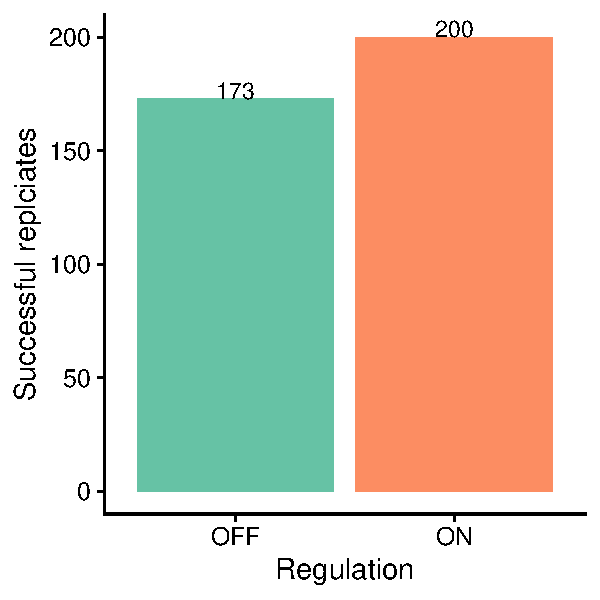
\includegraphics[width=\linewidth]{chapters/05-tag-based-genetic-regulation/media/context-signal-solution-counts.pdf}
    \caption{\small Successful replicates.}
    \label{chapter:tag-based-regulation:subfig:context-signal-solution-counts}
\end{subfigure}
\hfill
\begin{subfigure}[b]{0.45\textwidth}
    \centering
    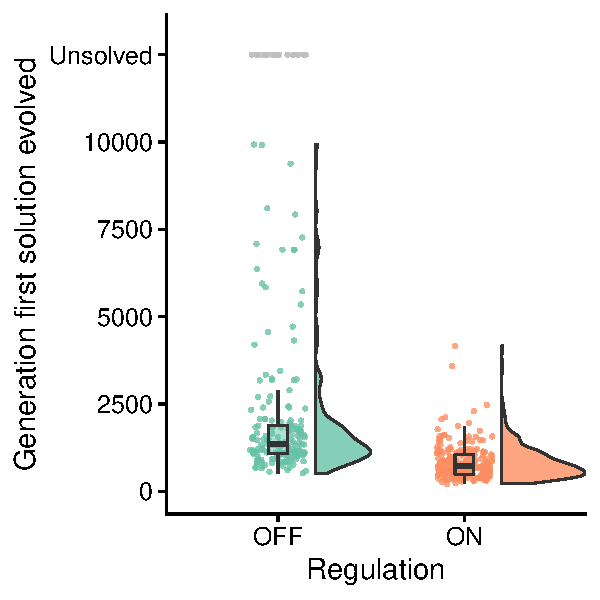
\includegraphics[width=\textwidth]{chapters/05-tag-based-genetic-regulation/media/context-signal-solve-time-cloud.pdf}
    \caption{\small Generations elapsed before solution.}
    \label{chapter:tag-based-regulation:subfig:context-signal-solve-time}
\end{subfigure}

\caption{\small 
\textbf{Contextual-signal problem-solving performance.}
(a) shows the number of successful replicates for the regulation-off and regulation-on conditions on the contextual-signal problem. 
The regulation-off condition was less successful than the regulation-on condition (Fisher's exact test: $p < 6\times10^{-9}$).
(b) is a raincloud plot showing the generation at which the first solution evolved in each successful replicate.
Gray points indicate the number of unsuccessful replicates for each condition.
Regulation-on solutions typically required fewer generations than regulation-off solutions to arise  (Wilcoxon rank sum test: $p < 10^{-15}$).
}

% problem-solving success - p-value = 5.818e-09; fisher's
% solve time: p-value < 2.2e-16; wilcoxon
    
\label{chapter:tag-based-regulation:fig:context-signal-performance}
\end{figure}


Figure \ref{chapter:tag-based-regulation:subfig:context-signal-solution-counts} shows the number of successful replicates on the contextual-signal problem for both the regulation-on and regulation-off conditions.
While both conditions were often successful, we found that access to tag-based regulation significantly improved problem-solving success.
Further, regulation-on solutions typically required fewer generations to evolve than regulation-off solutions (Figure \ref{chapter:tag-based-regulation:subfig:context-signal-solve-time}).

% (2) Solution strategies (knockouts)
We used knockout experiments to identify the mechanisms underlying each solution's strategy.
As expected, all 173 solutions evolved without access to tag-based regulation relied on their global memory buffer to track contextual information and used control flow mechanisms to differentiate their responses based on stored context.
Indeed, we found that regulation-off solutions executed a larger proportion of flow-control instructions than regulation-on solutions (Wilcoxon rank sum test: $p < 10^{-15}$; supplement \supSecContextSigAnalysis\ \citep{tag_regulation_supplement_2021}).
We also found that all 200 regulation-on solutions relied on tag-based regulation for response differentiation: 105 relied only on tag-based regulation and 95 relied on a combination of both tag-based regulation and global memory.
% Control flow proportions:
% p < p-value < 2.2e-16; 95% ci: 4.28% - 5.43%

In contrast to the signal-counting problem, we did not find that successful regulatory networks used primarily self-repressing modules.
Instead, we found that networks were more balanced between repressing and promoting edges; indeed, we found that successful networks generally contained more promoting edges than repressing edges (supplement \supSecContextSigAnalysis\ \citep{tag_regulation_supplement_2021}).
This result suggests that we should expect different problems to select for different forms of gene regulatory networks.

\subsubsection{Boolean-logic Calculator Problem}
\label{chapter:tag-based-regulation:sec:results:boolean-calc-problem}

% (1) solutions + solution timings

\begin{figure}[ht]
\centering

\begin{subfigure}[b]{0.45\textwidth}
    \centering
    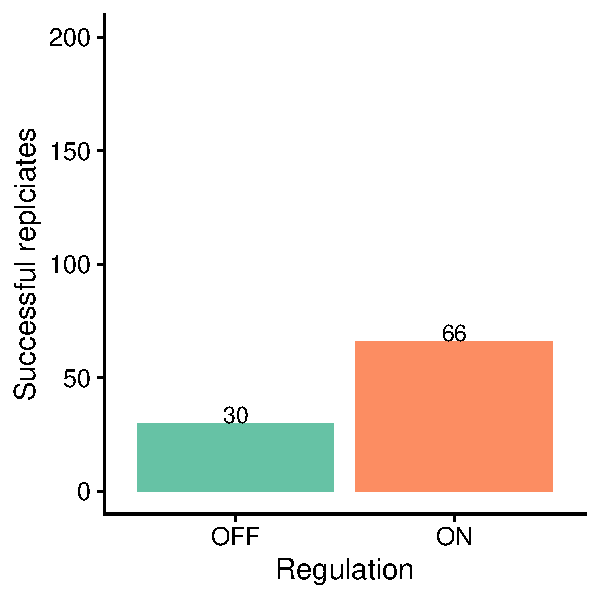
\includegraphics[width=\linewidth]{chapters/05-tag-based-genetic-regulation/media/boolean-calc-prefix-solution-counts.pdf}
    \caption{\small Successful replicates.}
    \label{chapter:tag-based-regulation:subfig:boolean-calc-prefix-solution-count}
\end{subfigure}
\hfill
\begin{subfigure}[b]{0.45\textwidth}
    \centering
    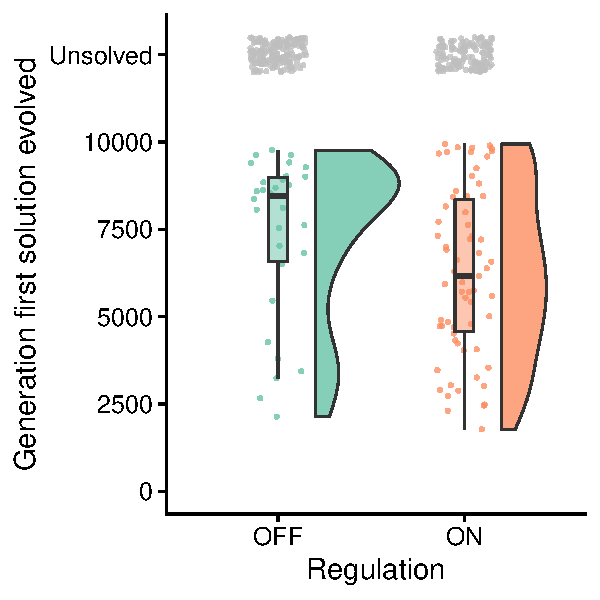
\includegraphics[width=\textwidth]{chapters/05-tag-based-genetic-regulation/media/boolean-calc-prefix-solve-time-cloud.pdf}
    \caption{\small Generations elapsed before solution.}
    \label{chapter:tag-based-regulation:subfig:boolean-calc-prefix-solve-time}
\end{subfigure}

\caption{\small
\textbf{Boolean-logic calculator problem-solving performance.}
(a) shows the number of successful replicates for the regulation-off and regulation-on conditions on the Boolean-logic calculator problem. 
The regulation-off condition was less successful than the regulation-on condition (Fisher's exact test: $p < 4\times10^{-05}$).
(b) is a raincloud plot showing the generation at which the first solution evolved in each successful replicate.
Gray points indicate the number of unsuccessful replicates for each condition.
Regulation-on solutions typically required fewer generations than regulation-off solutions to arise (Wilcoxon rank sum test: $p < 0.042$).
}

% fisher's  p-value = 3.585e-05
% wilcoxon rank sum: p-value = 0.04102
    
\label{chapter:tag-based-regulation:fig:boolean-calc-prefix-performance}
\end{figure}


Figure \ref{chapter:tag-based-regulation:subfig:boolean-calc-prefix-solution-count} shows the number of successful replicates on the Boolean-logic calculator problem for both the regulation-on and regulation-off conditions.
While both regulation-on and regulation-off solutions evolved, we again found that access to genetic regulation significantly improved problem-solving success.
Further, as in the signal-counting and contextual-signal problems, regulation-on solutions typically required fewer generations to evolve than regulation-off solutions (Figure~\ref{chapter:tag-based-regulation:subfig:boolean-calc-prefix-solve-time}).


\begin{figure}
\centering

\begin{subfigure}[b]{0.95\textwidth}
    \centering
    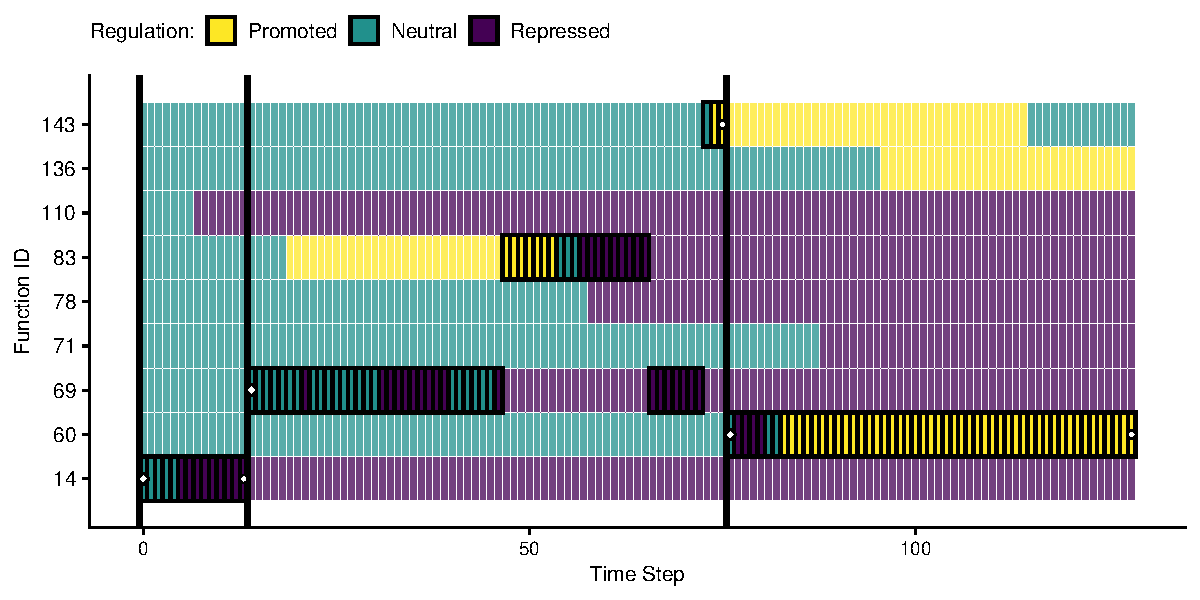
\includegraphics[width=\textwidth]{chapters/05-tag-based-genetic-regulation/media/boolean-calc-prefix-networks/case-study-trace-id-24400-test_id-420-regulator-state-horizontal.pdf}
    \caption{\small  Module regulation over time for a NAND operation.}
    \label{chapter:tag-based-regulation:subfig:bc-nand-exec-trace}
\end{subfigure}%

\begin{subfigure}[b]{0.5\textwidth}
    \centering
    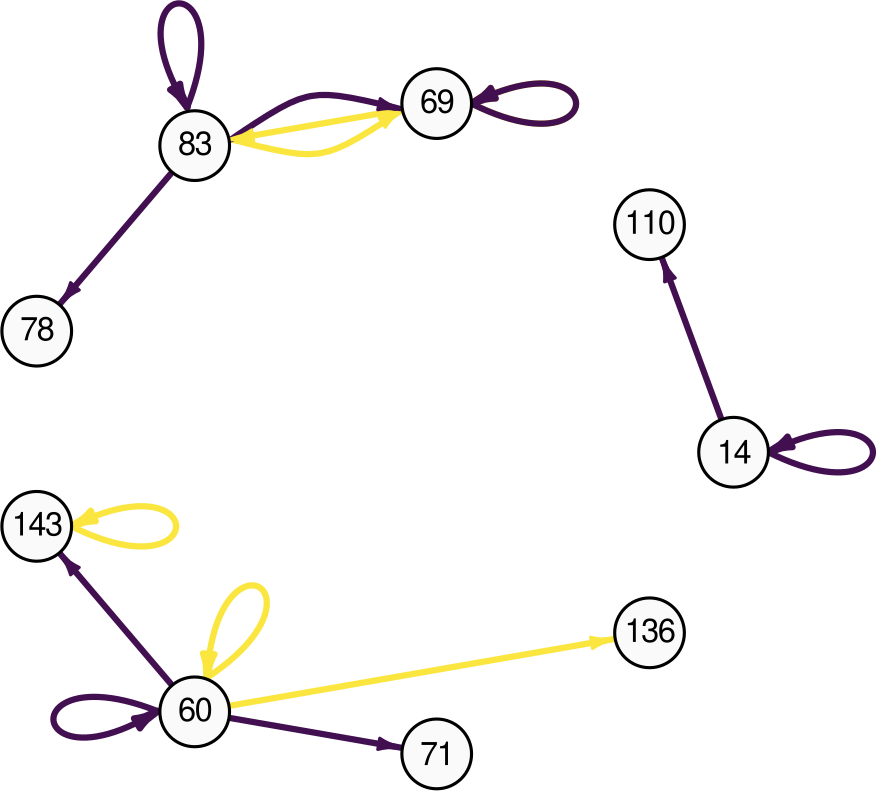
\includegraphics[width=0.6\textwidth]{chapters/05-tag-based-genetic-regulation/media/boolean-calc-prefix-networks/case-study-id-24400-test-420-network-cropped.png}
    \caption{\small NAND regulatory network.}
    \label{chapter:tag-based-regulation:subfig:bc-nand-reg-network}
\end{subfigure}%
\hfill
\begin{subfigure}[b]{0.5\textwidth}
    \centering
    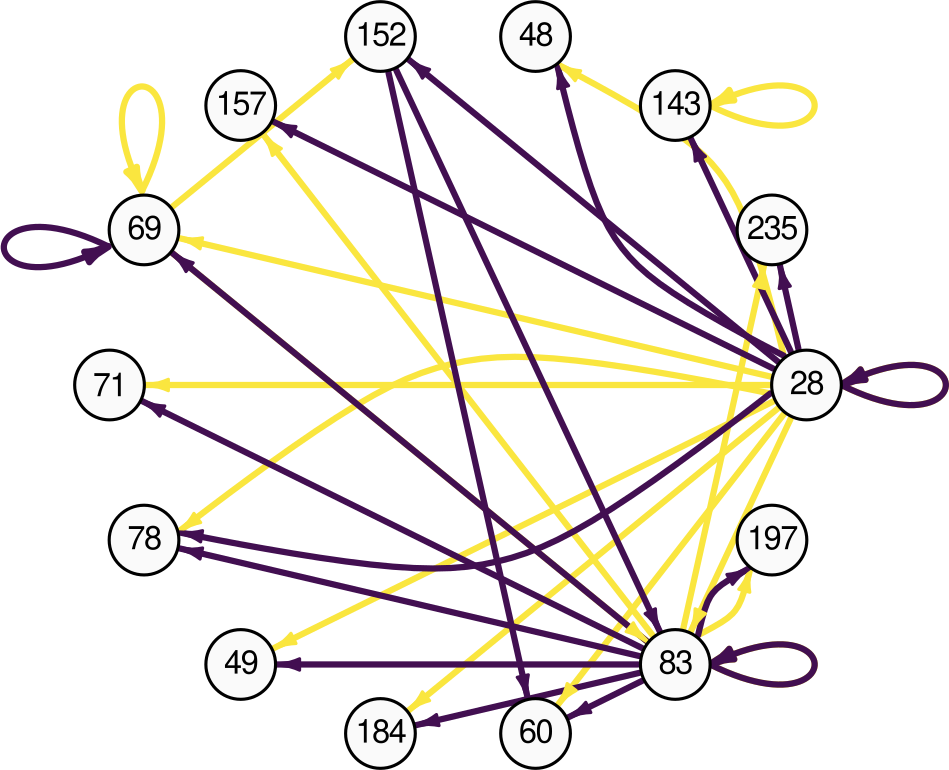
\includegraphics[width=0.6\textwidth]{chapters/05-tag-based-genetic-regulation/media/boolean-calc-prefix-networks/case-study-id-24400-test-134-network-cropped.png}
    \caption{\small NOR regulatory network.}
    \label{chapter:tag-based-regulation:subfig:bc-nor-reg-network}
\end{subfigure}%

\begin{subfigure}[b]{0.95\textwidth}
    \centering
    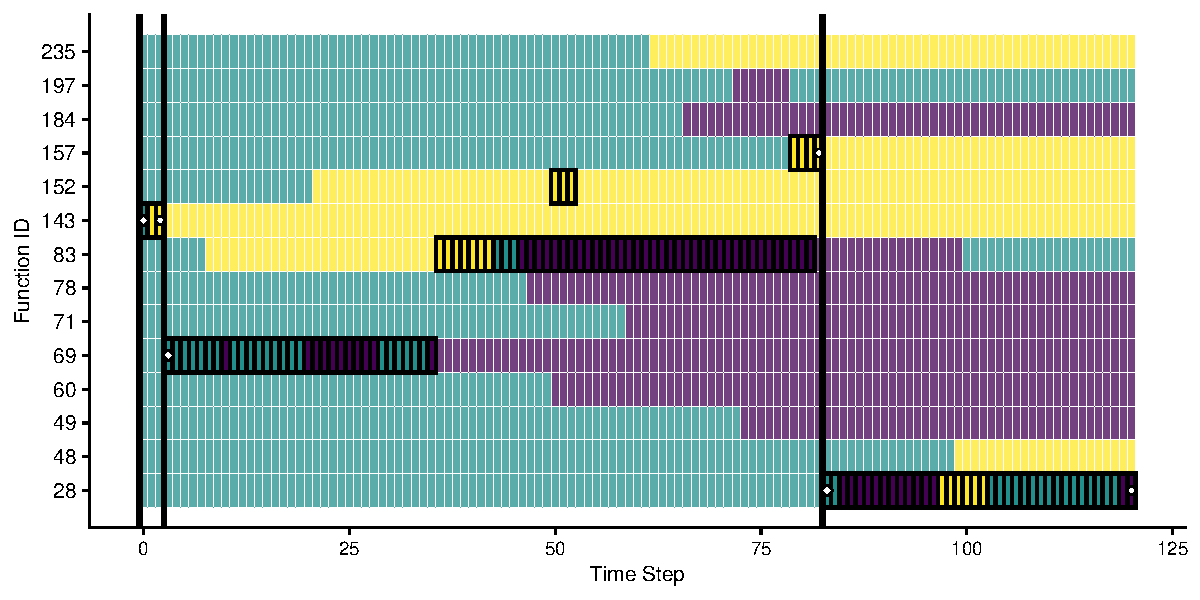
\includegraphics[width=0.95\textwidth]{chapters/05-tag-based-genetic-regulation/media/boolean-calc-prefix-networks/case-study-trace-id-24400-test_id-134-regulator-state-horizontal-nolegend.pdf}
    \caption{\small Module regulation over time for a NOR operation.}
    \label{chapter:tag-based-regulation:subfig:bc-nor-exec-trace}
\end{subfigure}%

\caption{\small 
\textbf{Execution traces of a successful SignalGP program computing a NAND operation (a) and a NOR operation (d).}
(b) and (c) show the directed graphs representing the regulatory networks associated with traces (a) and (d), respectively.
These visualizations are in the same format as those in Figure \ref{chapter:tag-based-regulation:fig:signal-counting-example-networks}.}
\label{chapter:tag-based-regulation:fig:boolean-calc-prefix-example-networks}
\end{figure}


As in previous experiments, we conducted knockout experiments to identify the mechanisms underlying each solution's strategy.
To compute any of the Boolean logic operations, programs \textit{must} make use of the global memory buffer to store numeric inputs (operands) to be used when performing the computation specified by the final operator signal. 
Indeed, all solutions evolved across all conditions relied on their global memory buffer to solve this problem.
All 66 regulation-on solutions, however, also relied on tag-based regulation to perform the appropriate computation for each test case.
Consistent with results from each other context-dependent problem, we found that regulation-off solutions executed a larger proportion of flow-control instructions than regulation-on solutions (Wilcoxon rank sum test: $p < 2\times10^{-05}$; supplement \supSecBooleanCalcPrefixAnalysis\ \citep{tag_regulation_supplement_2021}).
% Wilcoxon rank sum test: p-value = 1.328e-05 CI 1.486% - 3.91%

As in the signal-counting problem, we visualized the gene regulatory networks that manifest as a result of programs executing promoting and repressing instructions. 
Figure \ref{chapter:tag-based-regulation:fig:boolean-calc-prefix-example-networks} overviews the execution of a representative program evolved to solve the Boolean-logic calculator problem.
Specifically, Figure \ref{chapter:tag-based-regulation:fig:boolean-calc-prefix-example-networks} shows a program computing NAND and the same program computing NOR. 
The networks expressed on each of these operations are distinct despite originating from the same code.
These visualizations confirm that tag-based regulation allows programs to dynamically adjust their responses based on context (in this case, an initial operator signal). 

\subsection{Erroneous regulation can hinder task generalization}

In the signal-counting, contextual-signal, and Boolean-logic calculator problems, programs must adjust their behavior depending on the particular sequence of received signals.
The independent-signal problem, however, requires no signal-response plasticity; programs maximize fitness by statically associating $K$ distinct responses each with one of $K$ distinct input signals.
For this task, re-wiring signal-response associations within-lifetime is maladaptive.
As such, does the capacity for regulation impede adaptation to the independent-signal task?

We compared 200 replicate populations evolved with regulation-enabled SignalGP (``regulation-on'') and 200 populations evolved with regulation-disabled SignalGP (``regulation-off'').
All replicates produced a SignalGP program capable of achieving a perfect score during evaluation. 
We found no evidence that the availability of regulation affected the number of generations required to produce these solutions.

Next, we investigated how well evolved solutions \textit{generalized} across random permutations of input sequences.
Selection was deliberately based on a single stochastic ordering of environmental signals, so a ``perfect'' score may not generalize across all signal orderings.
We expect that programs evolved with access to regulation will more often exhibit non-adaptive plasticity that hinders generalization.

Figure \ref{chapter:tag-based-regulation:fig:independent-signal-generalization} shows the number of evolved solutions from each condition that successfully generalized.
All programs that evolved without access to regulation successfully generalized; however, evolved programs from 18 out of 200 successful regulation-on replicates failed to generalize beyond the test cases they experienced during evolution (Fisher's exact test: $p < 6\times10^{-6}$).
Moreover, 5 of 18 non-generalizing programs generalized when we knocked out tag-based regulation.
Upon closer inspection, the other non-general programs relied on tag-based regulation for initial success but failed to generalize to arbitrary environment sequences.
% fisher's p-value = 5.113e-06

\begin{figure}[ht]
    \centering
    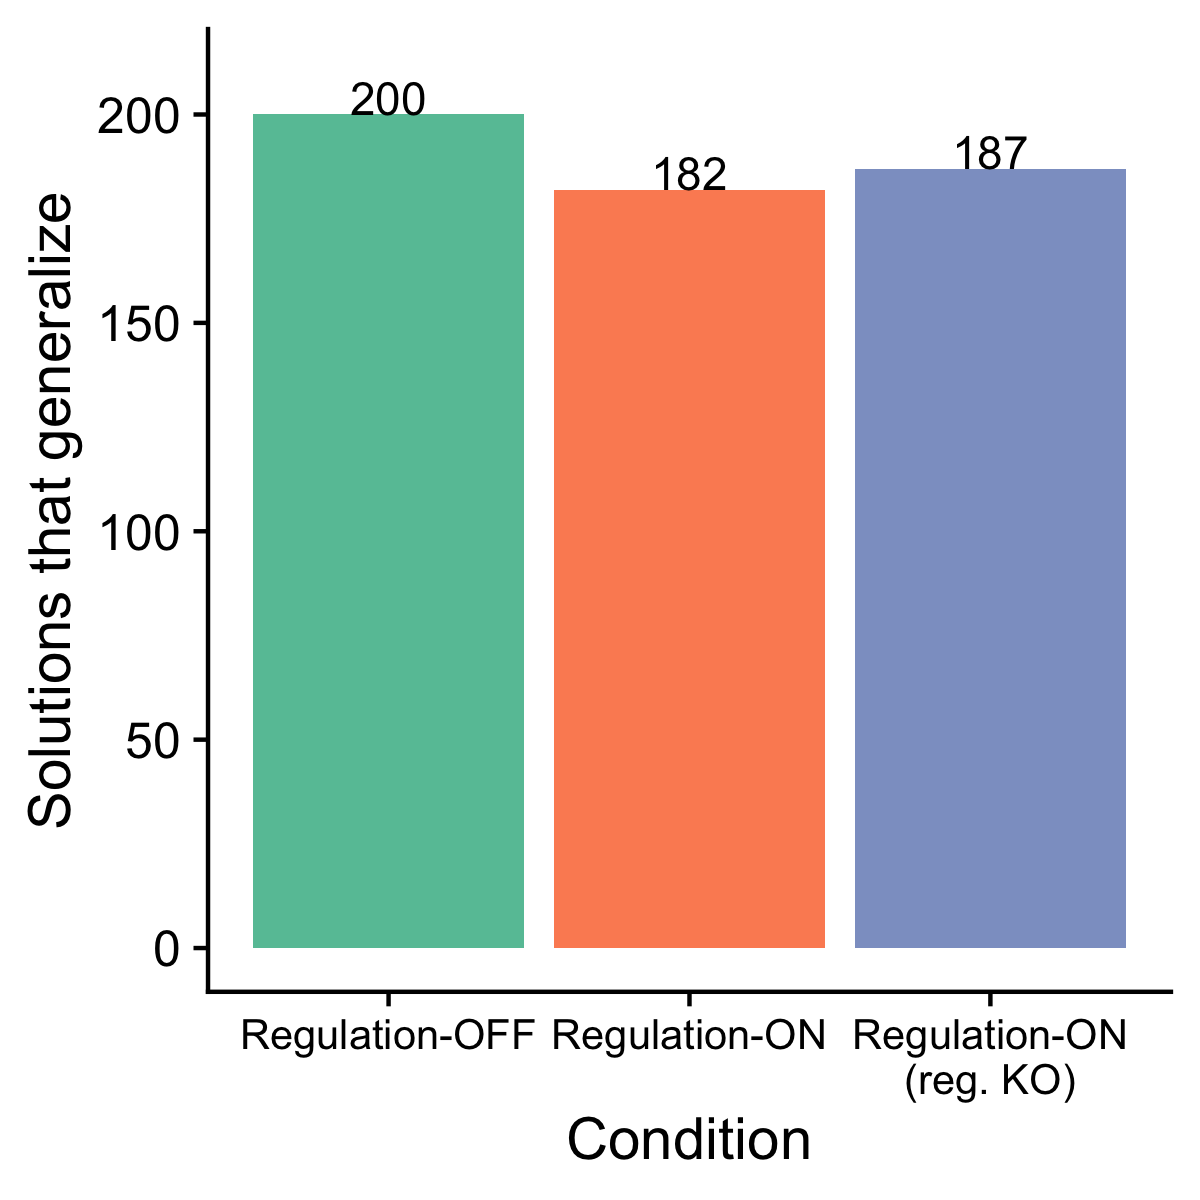
\includegraphics[width=0.5\textwidth]{chapters/05-tag-based-genetic-regulation/media/chg-env-16-generalization.png}
    \caption{\small
    \textbf{The number of evolved solutions that generalize on the independent-signal problem.}
    The difference in number of solutions that generalize between the regulation-on and regulation-off conditions is statistically significant (Fisher's exact test: $p < 6\times10^{-06}$).
    The ``Regulation-ON (reg. KO)'' condition comprises the solutions from the Regulation-on condition, except with regulatory instructions knocked out (\textit{i.e.}, replaced with no-operation instructions).
    }
    \label{chapter:tag-based-regulation:fig:independent-signal-generalization}
\end{figure}




Unexpressed traits that vary in a population (but do not affect fitness) are collectively known as cryptic variation. 
Cryptic variation is pervasive in nature and thought to play an important role in evolution, potentially acting as a cache of diverse phenotypic effects in novel environments \citep{gibson_uncovering_2004,paaby_cryptic_2014}.
Such cryptic variation has been shown to help GP systems escape local optima, improving overall problem-solving performance \citep{turner_neutral_2015}.
Cryptic variation arises when environmental conditions that would reveal the variation are not experienced. 
Access to tag-based regulation appears to make such cryptic variation in evolving programs a stronger possibility than previously.
This dynamic can be valuable for performing more realistic studies of evolutionary dynamics with digital organisms (\textit{i.e.}, self-replicating computer programs \citep{wilke_biology_2002}).
However, when using regulation-enabled SignalGP in problem-solving domains, such as automatic program synthesis, non-adaptive plasticity should be accounted for in fitness objectives.
In the independent-signal problem, for example, we could have performed more thorough evaluations of programs using multiple random permutations of input sequences instead of one.
In more challenging problems, however, more thorough evaluations can come at the cost of substantial computational effort. 

\begin{raggedright}
\subsection{Reducing the context required for the Boolean-logic calculator problem eliminates the benefit of regulation}
\end{raggedright}

Experimental results on the independent-signal problem suggest that enabling tag-based regulation is not necessarily beneficial for solving problems that do not require context-dependent responses to input. 
We use a modified version of the Boolean-logic calculator problem to further investigate the potential for tag-based regulation to impede adaptive evolution. 
The Boolean-logic calculator problem as described in Section \ref{chapter:tag-based-regulation:sec:methods:boolean-calc-problem} provides inputs in prefix notation: the operator (\textit{e.g.}, AND, OR, XOR, \textit{etc.}) is specified first, followed by the requisite number of numeric operands. 
As such, the final input signal does not differentiate which type of computation a program is expected to perform.
Programs must adjust their response based on the context provided by previous signals, thereby increasing the utility of regulation. 

Here, we explore whether the calculator problem's context-dependence is driving the benefit of tag-based regulation that we identified in Section \ref{chapter:tag-based-regulation:sec:results:boolean-calc-problem}.
We can reduce context-dependence of the calculator problem by presenting input sequences in \textit{postfix} notation. 
In postfix notation, programs receive the requisite numeric operand inputs first and the operator input last. 
As such, the final signal in an input sequence will always differentiate which bitwise operation should be performed.
Successful programs must store the numeric inputs embedded in operand signals, and then, as in the independent-signal problem, a distinct signal will differentiate which of the response types a program should execute. 

\begin{figure}[ht]
\centering

\begin{subfigure}[b]{0.45\textwidth}
    \centering
    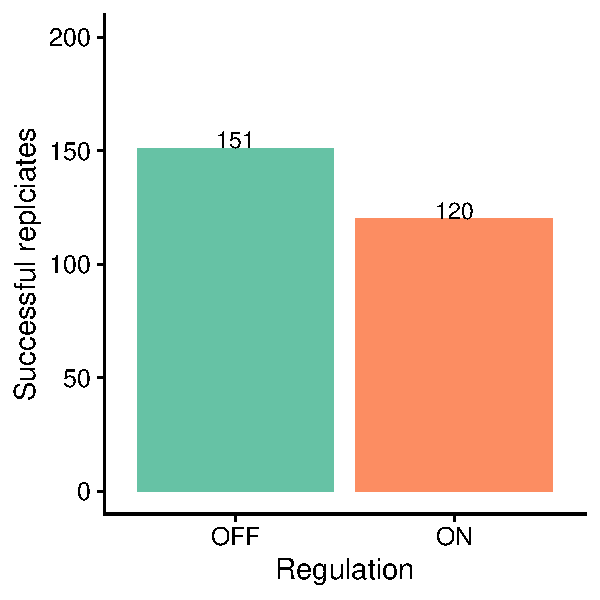
\includegraphics[width=\linewidth]{chapters/05-tag-based-genetic-regulation/media/boolean-calc-postfix-solution-counts.pdf}
    \caption{\small Successful replicates.}
    \label{chapter:tag-based-regulation:subfig:boolean-calc-postfix-solution-count}
\end{subfigure}
\hfill
\begin{subfigure}[b]{0.45\textwidth}
    \centering
    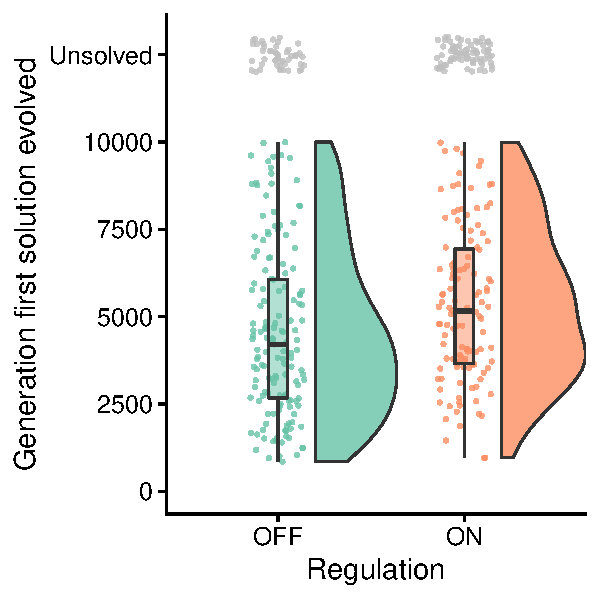
\includegraphics[width=\textwidth]{chapters/05-tag-based-genetic-regulation/media/boolean-calc-postfix-solve-time-cloud.pdf}
    \caption{\small Generations elapsed before solution.}
    \label{chapter:tag-based-regulation:subfig:boolean-calc-postfix-solve-time}
\end{subfigure}

\caption{\small 
\textbf{Boolean-logic calculator (postfix notation)  problem-solving performance.}
(a) shows the number of successful replicates for the regulation-off and regulation-on conditions on the postfix Boolean-logic calculator problem. 
The regulation-on condition was less successful than the regulation-off condition (Fisher's exact test: $p<0.002$).
(b) is a Raincloud plot showing the generation at which the first solution evolved in each successful replicate.
Gray points indicate the unsuccessful replicates for each condition.
Regulation-off solutions typically required fewer generations than regulation-on solutions to arise (Wilcoxon rank sum test: $p<0.004$).
}
% fisher's exact: p-value = 0.001286
% wilcoxon:  p-value = 0.003285
\label{chapter:tag-based-regulation:fig:boolean-calc-postfix-performance}
\end{figure}


We repeated the Boolean-logic calculator experiment (as described in Section \ref{chapter:tag-based-regulation:sec:methods:boolean-calc-problem}), except we presented inputs in postfix notation instead of prefix notation. 
Figure \ref{chapter:tag-based-regulation:subfig:boolean-calc-postfix-solution-count} shows the number of successful replicates evolved in regulation-on and regulation-off conditions.
Postfix notation decreases the overall difficulty of the Boolean-logic calculator problem; more solutions evolved in each condition than evolved with prefix notation (Section \ref{chapter:tag-based-regulation:sec:results:boolean-calc-problem}).
We found that the regulation-on condition resulted in lower problem-solving success than the regulation-off condition. 
We also found that regulation-off solutions typically required fewer generations than regulation-on solutions to arise (Figure \ref{chapter:tag-based-regulation:subfig:boolean-calc-postfix-solve-time}).
Additionally, we did not observe a significant difference in the proportion of flow-control instructions represented in execution traces of regulation-on and regulation-off solutions (supplement \supSecBooleanCalcPostfixAnalysis\ \citep{tag_regulation_supplement_2021}). 

These results, in combination with our previous experimental results, suggest that tag-based regulation is beneficial when prior context dictates behavioral responses to input.
On such context-dependent problems, representations without explicit regulation must compensate with additional conditional logic structures. 
\section{Conclusion}

% - Positive results, immediately applicable to other tag-enabled systems -
We demonstrated that tag-based genetic regulation allows GP systems to evolve programs with more dynamic plasticity.
These evolved programs are better able to solve context-dependent problems where the appropriate software modules to execute in response to a particular input changes over time.
Genetic regulation broadens the applicability of SignalGP, both as a representation for problem-solving and as a type of digital organism for studying evolutionary dynamics \citep{Lalejini_Moreno_Ofria_DISHTINY_2020}.
Further, this work illustrates an approach for easily incorporating tag-based models of gene regulation into existing GP systems. 

% - negative results, future work on matching schemes -
Our results also reveal that tag-based regulation is not necessarily beneficial across all problem domains.
We observed that the addition of tag-based regulation can impede adaptive evolution on problems where responses to inputs are not context-dependent (\textit{e.g.}, the independent-signal task and postfix version of the Boolean-logic calculator problem). 
A more thorough examination of what types of context-free problems are most sensitive to tag-based regulation---and how to mitigate any harm---would be potentially fruitful.

% ---- BEGIN REVISION ----
% - issues with existing representations -
Across all problems used in this work, the tag representation and matching scheme that we used was clearly sufficient for success. 
However, existing tag systems are limited in their capacity to scale up to substantially larger gene regulatory networks. 
As these networks grow, the specificity required for references to differentiate between modules increases. 
At some point references become brittle, as any mutation will switch the module that a call triggers.
In ongoing work, we are investigating the wide variations in scalability of different metrics for measuring the similarity between tags.
Substantial work will also need to be conducted by the community in order to develop more scalable representations for tag-based naming.
% @AML: new line below (currently very weak sentence)
For example, insights from the indirect referencing mechanisms of artificial biochemical networks and enzyme genetic programming systems may prove to be informative in developing new tag representations \citep{lones_modelling_2004,lones_artificial_2014,lones_biochemical_2013}.
% --- END REVISION ----

% ---- BEGIN REVISION ----
% - Comment: Another thing that would be good to comment on is the interpretability of the evolved solutions. I'm guessing that the regulatory-based solutions are harder for humans to understand?
% @AML: needs work!!
Evolved programs are often more challenging to read and understand than programs written by human developers.
In our experience, evolved programs that make use of tag-based regulation were substantially more difficult to read and interpret by hand than evolved programs that do not use tag-based regulation.
We found that visualizations of tag-based regulatory networks and program execution traces (\textit{e.g.}, Figures \ref{chapter:tag-based-regulation:fig:signal-counting-example-networks} and \ref{chapter:tag-based-regulation:fig:boolean-calc-prefix-example-networks}) improved our ability to understand how a given evolved program worked.
As we scale up tag-based regulation, the development of interactive visualizations will become increasingly important for understanding evolved programs that make use of tag-based regulation.  
% ---- END REVISION -----

The current investigations have focused on regulation as a problem-solving tool, but with a few extensions these sorts of systems can also help us answer open questions about biological evolution.
Our current implementation of tag-based regulation facilitates plasticity only within a program's lifetime; if we extend this capacity across multiple generations, we can study the effects of epigenetic inheritance on evolutionary dynamics.
Epigenetic inheritance refers to heritable phenotypic changes that are not directly encoded by the underlying genetic sequence \citep{bender_plant_2002,jablonka_transgenerational_2009}.
For example, epigenetics is used in combination with gene regulation for cell-type differentiation in multicellular organisms \citep{mohn_genetics_2009, smith_dna_2013} and caste determination in some species of eusocial insects \citep{weiner_epigenetics_2012}.
SignalGP supports epigenetics with the addition of instructions that mark existing function regulation as heritable.
For our next steps, we will apply epigenetics-enabled SignalGP to study fraternal transitions in individuality and the evolution of differentiation before, during, and after a transition occurs \citep{Lalejini_Moreno_Ofria_DISHTINY_2020}.
Open-ended experiments with epigenetics and gene regulation will help illuminate the relationship between within-lifetime plastic adaptation and evolutionary adaptation over generational time scales.
Additionally, mechanisms for epigenetic inheritance have been shown to potentially improve GP performance \citep{la_cava_genetic_2015, la_cava_inheritable_2015,ricalde_evolving_2017}; as such, we plan to apply our insights back to automatic program synthesis. 

\chapter{Tag-accessed Memory for Genetic Programming}
\label{chapter:tag-accessed-memory}

\noindent
Authors: Alexander Lalejini and Charles Ofria \\
This chapter is adapted from ~\citep{lalejini_tag-accessed_2019}, which appeared in the companion proceedings of the 2019 Genetic and Evolutionary Computation Conference.

\section{Introduction}

Here, we demonstrate the use of tags (evolvable labels that can be specified with imperfect matching) to identify memory positions in genetic programming (GP).
Specifically, we conducted a series of experiments using simple linear-GP representations on five problems from the general program-synthesis benchmark suite~\citep{helmuth_general_2015}.  
We show that tag-indexed memory does not substantively affect problem solving success relative to more traditional, direct-indexed memory.

In traditional software engineering, human programmers create variables with unique names to specify data that they are working with.  
These variables are inherently associated with locations in memory that are accessed by using the variable's name.
This technique for referencing values in memory is intentionally rigid, requiring programmers to precisely name the data they want to reference, and imprecision results in syntactic errors.
Many traditional GP systems that give genetic programs access to memory (\textit{e.g.}, indexable memory registers) use similarly rigid naming schemes where memory is numerically indexed, and mutation operators must guarantee the validity of memory-referencing instructions. 
Interestingly, although exact naming is the most intuitive referencing mechanism
for human programmers, evolution in other contexts (such as identifying modules to run~\citep{lalejini_what_2019}) has been shown to be more successful when program references are allowed to be inexact.
Beyond computer code, robustness to perturbations is also thought to be important in the evolution of complex biological systems~\citep{kitano_biological_2004}.

\begin{figure}
  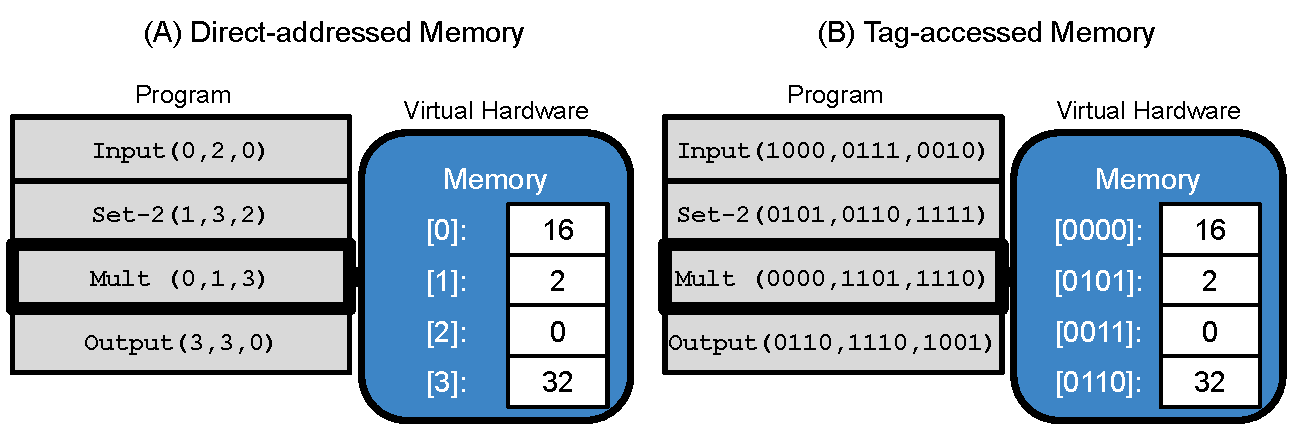
\includegraphics[width=1.0\columnwidth]{chapters/06-tag-access-memory/media/memory-access-overview.pdf}
  \caption{\small 
  Examples of (A) direct-indexed memory and (B) tag-accessed memory. 
  The programs in (A) and (B) behave identically: both request input to the first memory register, set the second memory register to the terminal value `2', place the result of multiplying the contents of the first two memory registers into the fourth memory register, and output the contents of the fourth register.
  Here, we show the state of memory after the \code{Mult} instruction has been executed. 
  Note that not all instructions use all three arguments.
  }
  \label{chapter:tag-accessed-memory:fig:memory-access-overview}
\end{figure}

% @AML: Here is where I describe tags and tag-based references.
Tags are evolvable labels that give genetic programs a flexible mechanism for specification, originally used by Holland in genetic algorithms (\citep{holland_effect_1993}) and refined by Spector \textit{et al.} for GP~\citep{spector_tag-based_2011}.
To facilitate \textit{inexact} referencing, the similarity (or dissimilarity) between any two tags must be quantifiable; a referring tag can always reference the closest matching referent tag.
Here, we continue to expand the integration of tags into linear GP by allowing instructions to use tags to identify positions in memory (as needed for their function).
All instructions have three tag-based arguments, each of which is represented as a length-16 bit string and compared using Hamming distance to measure similarity.
Our instruction set allows programs to perform basic computations, manipulate memory contents, and control execution flow (see supplemental material~\citep{tag_accessed_memory_supplement_2019} for details).
Programs are executed in the context of a virtual CPU that gives them access to 16 statically tagged memory registers used for storing data for performing computations.
Figure \ref{chapter:tag-accessed-memory:fig:memory-access-overview} contrasts tag-based memory with direct-indexed memory.
Tag-based instruction arguments reference the memory position with the \textit{closest matching} tag; as such, argument tags need not \textit{exactly} match any of the tags associated with memory positions.
This inexactness makes program phenotypes more robust to minor genetic perturbations, smoothing the genotype-phenotype mapping relative to more traditional memory-indexing techniques.

\section{Experimental Results}

We compared the performance of our simple linear GP to a variant that replaced the tag-accessed memory with memory indexed with direct arguments (which is more akin to memory access in traditional linear GP~\citep{brameier_linear_2007}).
We evolved programs using the lexicase parent selection algorithm~\cite{helmuth_solving_2015} to solve five problems from Helmuth and Spector's program synthesis benchmark suite~\citep{helmuth_general_2015}: number IO, smallest, median, grade, and for loop index.
For each problem, we added custom instructions to the instruction set that facilitated loading test case inputs into memory and returning program responses. 
We used the same training and testing sets when evaluating programs as Helmuth and Spector in~\citep{helmuth_general_2015}.
We measured performance by counting the number of successful runs (\textit{i.e.}, runs that produced a perfect solution).%, and we tested for statistical significance using Fisher's exact test (with a significance threshold of 0.05).

For each experimental condition, we evolved 50 replicate populations of 500 individuals (for 100 generations for the number IO problem and 500 generations for all other problems), giving each replicate a unique random number seed.
We propagated programs asexually and applied mutations to offspring (single-instruction insertions, deletions, and substitutions at a per-instruction rate of 0.005 each and multi-instruction sequence duplications and deletions at a per-program rate of 0.05). 
The relative success of these two memory-indexing techniques is influenced by how (and at what rate) we mutate instruction arguments.
As such, we mutated tag-based arguments (per-bit) and traditional arguments (per-argument) at the following ten rates: 0.0001, 0.001, 0.0025, 0.005, 0.0075, 0.01, 0.025, 0.05, 0.075, and 0.1. 
See our online supplemental material \citep{tag_accessed_memory_supplement_2019} for source code, details on problem-specific configurations (\textit{e.g.}, program evaluation time, \textit{etc.}), and for our more detailed analyses.

\begin{figure}
  \centering
  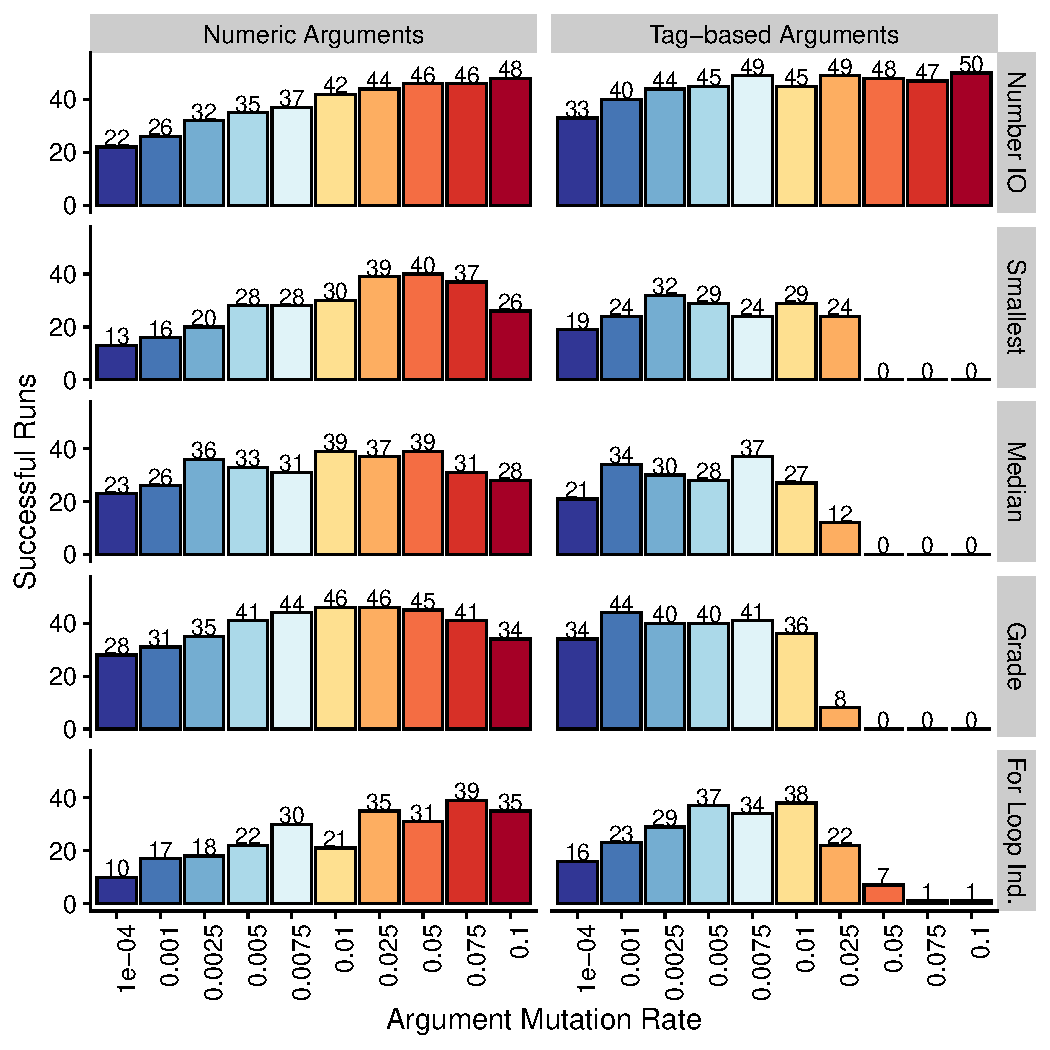
\includegraphics[width=0.75\columnwidth]{chapters/06-tag-access-memory/media/problem-solving-success.pdf}
  \caption{\small 
  \textbf{Number of successful runs} when using our tag-accessed memory (right column) versus using traditional direct-indexed memory (left column) across five problems and ten instruction argument mutation rates (after 100 generations for number IO and 500 generations for all other problems).
  }
  \label{chapter:tag-accessed-memory:fig:successful-runs}
\end{figure}

Figure \ref{chapter:tag-accessed-memory:fig:successful-runs} shows the performance of tag-accessed memory and direct-indexed memory for each problem and mutation rate.
For each problem, we selected the best (most successful) mutation rate for tag-based arguments and the best mutation rate for traditional arguments.
We compared the performance of tag-based arguments and numeric arguments at these ``optimal'' mutation rates, and we tested for we tested for statistical significance using Fisher's exact test (with a significance threshold of 0.05). 
Across all problems, there was no statistically significant difference between tag-based instruction arguments (tag-accessed memory) and numeric instruction arguments (direct-indexed memory).

Figure \ref{chapter:tag-accessed-memory:fig:successful-runs} also seems to indicate that tag-accessed memory is more sensitive to mutation rate than direct-addressed memory. 
Indeed, on the smallest, median, and grade problems, three mutation rates resulted in no solutions in our tag-based argument treatment, whereas all mutation rates in the numeric arguments treatment resulted in at least one solution on all problems.  
This result does not \textit{necessarily} indicate that tag-based arguments are less mutationally robust than numeric arguments.
We mutated numeric arguments at a per-argument rate, and as such, a mutation rate of 0.1 is an expected one mutation for every ten arguments mutated. 
We mutated tag-based arguments at a \textit{per-bit} rate, and as such, a mutation rate of 0.1 is an expected one to two bit flips per mutated tag. 
That is, in practice, the 0.1 per-bit mutation rate for tags is substantially higher than the 0.1 per-argument mutation rate for numeric arguments.
More experiments are needed to quantify tag-based argument and numeric argument sensitivity to mutation.  
% @AML: One more sentence about problem solving success?
\section{Conclusion}

Our preliminary experiments show that, under favorable mutation rates, both tag-accessed and direct-indexed memory achieve statistically equivalent performance.
Because tag-based instruction arguments index into the \textit{closest matching} memory register, single bit-flip mutations may be neutral (not affecting the program's behavior), which affords programs robustness to minor genetic perturbations. 
The down-side to a more robust genetic encoding for instruction arguments is that mutations are less able to generate novel phenotypic variation (program behavior).
For the relatively simple program synthesis problems used in our experiments, the capacity of our GP system to generate novel phenotypic variation is likely more important than robustness to mutation. 
Future work will continue to explore the efficacy of tag-accessed memory, supplementing bit-flip mutation operators with more impactful mutation operators that allow tag-mutations to more easily generate novel phenotypic variation.
Future work will also investigate the possibility of coevolving register labels (tags) with programs, allowing evolution to adjust the adjacency of memory registers in tag-space.
\chapter{Conclusions}
\label{chapter:conclusions}
%%%%%%%%%%%%%%%%%%%%%%%%%%%%% NOTES %%%%%%%%%%%%%%%%%%%%%%%%%%%%%
% All natural environments subject populations to some form of change.

% ; our findings suggest that the stabilizing effect of phenotypic plasticity plays an important role in subsequent adaptive evolution.

% mention DISHTINY
% mention lexicase 
% AAGOS understanding changing environments
%%%%%%%%%%%%%%%%%%%%%%%%%%%%% NOTES %%%%%%%%%%%%%%%%%%%%%%%%%%%%%

% TODO

Dissertation is split between two synergistic focuses: [blah] and [blah].
[Riff on Thesis statement].
[How I have achieved thesis statement].

\section{Contributions}

In summary, this dissertation makes the following contributions:

\begin{itemize}
    % --- Origins of plasticity ---
    \item In \textbf{Chapter \ref{chapter:evolutionary-origins-of-phenotypic-plasticity}}, [I/We?] found that both environmental change rate and mutation rate influence the likelihood for adaptive phenotypic plasticity to evolve in populations of digital organisms. 
    By analyzing the lineages of plastic organisms, I identified unconditional trait expression and imperfect forms of phenotypic plasticity as important evolutionary building blocks for the evolution of adaptive plasticity. 
    
    % --- Consequences of plasticity ---
    \item In \textbf{Chapter \ref{chapter:evolutionary-consequences-of-plasticity}}, I used populations of digital organisms to empirically test whether the evolution of adaptive phenotypic plasticity alters evolutionary dynamics and influences evolutionary outcomes in cyclically changing environments.
    I found that the evolution of adaptive phenotypic plasticity stabilizes populations against environmental changes and constrains the rate of subsequent evolutionary change.
    By buffering populations against environmental change, adaptive plasticity improved novel trait retention and reduced the accumulation of deleterious mutations relative to non-plastic populations evolved in an otherwise identical environment. 
    
    % --- SignalGP ---
    \item In \textbf{Chapter \ref{chapter:signalgp}}, I introduced SignalGP, a novel genetic programming technique for evolving event-driven computer programs. 
    I showed that SignalGP allows us to evolve programs better able to rapidly interact the environment or with other agents. 
    % Further, SignalGP model digital organism. 
    
    % --- Tag-based genetic regulation ---
    \item In \textbf{Chapter \ref{chapter:tag-based-regulation}}, I developed tag-based genetic regulation, a new genetic programming technique that allows programs to dynamically adjust which code modules to express.
    I described how to augment existing genetic programming systems with tag-based regulation, and I showed that tag-based regulation improves problem-solving performance on context-dependent problems where programs must adjust how they respond to current inputs based on prior inputs.
    
    % --- Tag-accessed memory ---
    \item In \textbf{Chapter \ref{chapter:tag-accessed-memory}}, I proposed tag-accessed memory, a new mechanism for labeling and identifying memory positions in genetic programming.  
    With preliminary experiments, I found that, under favorable mutation rates, both tag-accessed memory and conventional direct-indexed memory achieve similar performance on a range of program synthesis problems. 
    % [Promising technique for future research].
    
\end{itemize}

\section{Future Directions}

% TODO

Thus far, I have...

\subsection{Broadened applications of SignalGP}

% [Origins of SignalGP].
% - Cell biology class, learning about signal transduction.
% - Working on a project exploring different levels of complexity in plasticity using Avida, but having trouble evolving program capable of effectively independently regulating many tasks in environment. 
% - ROS (event-driven computing).
% - But how 
% - Use bit string signatures to match 
% - Tag-based referencing.

% I have shown it to be effective at X/Y/Z. 
% + added genetic regulation.

% Several next steps:

\subsubsection{Multi-representation SignalGP}
% \label{chapter:conclusion:sec:future-work:multi-representation-signalgp}

In Chapters \ref{chapter:signalgp} and \ref{chapter:tag-based-regulation}, I have exclusively used SignalGP in the context of linear GP.
That is, SignalGP functions (modules) associate a tag with a linear sequence of instructions. 
However, in principle, SignalGP is generalizable across a variety of evolutionary computation representations. 

SignalGP programs are composed of a set of functions where each function is referred to via its tag. 
We can imagine these functions to be black-box input-output machines: when called or triggered by an event, a function is run with input and can produce output by manipulating memory or by generating signals. 
Instead of constructing functions with linear sequences of instructions, I could used other computational substrates (representations) capable of receiving input and producing output (\textit{e.g.}, other GP representations, artificial neural networks, Markov Brains [cite - Hintze2017], hard-coded modules, \textit{etc.}). 
We could even employ a variety of representations within a single SignalGP agent. 

SignalGP's tag-based naming scheme allows us to use this black-box metaphor. 
Functions composed of different representations can still refer to one another via tags, and events are agnostic to the underlying representation used to handle them, requiring only that the representation is capable of processing event-specific data. 
Allowing for such multi-representation agents may complicate the SignalGP virtual hardware, program evaluation, and mutation operators, but in exchange, it would provide evolution with a toolbox of diverse representations. 

Hintze \textit{et al.} proposed and demonstrated the evolutionary ``buffet method'' where Markov brains could be composed of heterogeneous computational substrates, allowing evolution to work out the most appropriate representation for a given problem \citep{hintze_buffet_2019}. 
Indeed, Hintze \textit{et al.} observed that different problems produced solutions with different distributions of component types, making buffet-style Markov brains a flexible representation for solving a range of different types of problems. 
Multi-representation SignalGP provides an unexplored, alternative approach to evolving multi-representation agents, bringing the buffet method into an event-driven context.

\subsubsection{Major Transitions in SignalGP}

In a major evolutionary transition in individuality, formerly distinct individuals unite to form a new, more complex lifeform, redefining what it means to be an individual. 
The evolution of eukaryotes, multi-cellular life, and eusocial insect colonies are all examples of transitions in individuality. 
Often the individuals that make up the higher-level entity are limited to local information, lacking direct access to the global state of the higher-level unit; lower-level units must rely on signaling and sensory information to coordinate their roles in the group [cite - Smith1997,West2015].
In a computational sense, a major transition in individuality is the evolution of a distributed system.
Capturing these types of transitions in GP would give evolution a mechanism to incrementally form distributed systems from formerly individual programs. 

Above, I described how SignalGP could be extended to allow multi-representation programs where functions can be of any representation capable of receiving input and producing output. 
We can take this approach one step further: any module within a SignalGP agent could be \textit{another} (formerly individual) SignalGP agent. 
% This approach is conceptually similar to Tangled Program Graph representation \citep{Kelly2017}.
 
% \begin{figure*}
% 	\centering
%   \includegraphics[width=0.5\textwidth]{sgp-trans.pdf}
%   \caption{\small \textbf{Example of a multi-level SignalGP program.} In this example, the agent is composed of five modules, including a neural network, a Markov Brain, a linear GP representation, and two multi-module programs at a lower level of organization.}
%   \label{fig:major_trans_cartoon}
% \end{figure*}

For example, we can imagine a mutation operator that, when applied, induces transitions in individuality by injecting co-evolving SignalGP programs as self-contained, tagged modules into a mutated program, allowing single individuals to be aggregates of lower-level individuals. 
Further, transitions in individuality can be applied \textit{hierarchically}. 
Biological evolution has examples of such hierarchical transitions: eusocial insect colonies are composed of many multicellular individuals, each of which are composed of many eukaryotic cells, which in turn are composed of organelles (many of which are thought to have been formally distinct individuals).
An individual SignalGP program may be composed of many SignalGP program modules, which may themselves be composed of many SignalGP programs. 

Implementing a mutation operator capable of inducing arbitrary numbers of hierarchical transitions in individuality requires us to answer the following questions: 
How should formerly individual programs interact when forced into an aggregate? 
And, how should an evolutionary algorithm handle evaluating both individuals and aggregates of individuals? 

From the evolutionary algorithm's perspective, a multi-level SignalGP program is indistinguishable from a single-level. 
However, just as biological organisms composed of lower-level units of individuality require more energy to subsist, multi-level SignalGP programs require many more CPU cycles than single-level SignalGP programs. 
This is consistent with biology where major transitions disproportionately occur in energy-rich environments [cite - Smith1997]. 

Extending SignalGP to support hierarchical transitions in individuality could also provide a useful model for studying biological evolutionary transitions, allowing us to ask general questions about their dynamics. 
A transition in individuality mutation operator would also allow us to solve problems that might be best solved by a distributed system without knowing the optimal configuration of that distributed system \textit{a priori}. 

\subsubsection{SignalGP as a new model digital organism}

% TODO

\subsection{The evolutionary origins and consequences of phenotypic plasticity}


 
% - Signal-driven genetic programs as a model digital organism. 

\subsection{Applying evolutionary algorithms to microbial populations}



%%%  Appendices, if necessary:

% \begin{centering}
% \vfill
% \appendix{APPENDICES}                      %Make sure the names in
% \addcontentsline{toc}{chapter}{APPENDICES} %brackets match
% \vfill
% \end{centering}
% \newpage
% \input{appendix/appendix} %====Put you Appendix text here
% \clearpage


%\pagenumbering{gobble}% Remove page numbers (and reset to 1)
%%%  Bibliography:
\addcontentsline{toc}{chapter}{BIBLIOGRAPHY}

\newpage
\vspace*{\fill}
\begin{center}
BIBLIOGRAPHY
\vspace*{\fill}
\end{center}

\newpage
\begin{singlespace}
\bibliographystyle{apalike}% your bst file here
\bibliography{references,software} %your bib file here
\end{singlespace}
\end{doublespace}
\end{document}
